%La compilacion se debe hacer con la instruccion de PdfLatex
% para evitar problemas de tamaño de hoja.
% Todos los archivos de figuras deben estar en formato PDF.
% Al momento de imprimir el documento, se debe hacer sin escala de pagina.
\documentclass[letterpaper,12pt]{cicese}
%%%%%%%%%%%%%%%%%%%%%%%%%%%%%%%%%%%%%%%%%%%%%%%%%%%%%%%%%%%%%%%%%%%%%%%%%%%%%%%%%%%%%%%%%%%%%%%%%%%%%%%%%%%%%%%%%%%%%%%%%%%%%%%%%%%%%%%%%%%%%%%%%%%%%%%%%%%%%%%%%%%%%%%%%%%%%%%%%%%%%%%%%%%%%%%%%%%%%%%%%%%%%%%%%%%%%%%%%%%%%%%%%%%%%%%%%%%%%%%%%%%%%%%%%%%%
\usepackage{ marvosym }
\usepackage[letterpaper,left=3cm,right=2cm,top=2cm,bottom=1.3cm]{geometry}
%%\usepackage[ansinew]{inputenc}   %este paquete es para poner acentos directamente en el codigo de latex. sin barra
%\usepackage[T1]{fontenc}
%\usepackage[spanish,english]{babel}
%%\usepackage[spanish,mexico,es-lcroman]{babel}
%paquete para insertar hipervinculos en referencias a capitulos, figuras, etc.
\usepackage{helvet}
\renewcommand{\familydefault}{\sfdefault} 
\usepackage[spanish, mexico,es-lcroman]{babel}
\usepackage[utf8x]{inputenc}
\usepackage{mdframed}
\usepackage[acronym]{glossaries}
\makeglossaries
\usepackage[linkcolor=blue]{hyperref}
\usepackage{cicese}
%\usepackage{tabularx}
\usepackage{pbox}
\usepackage{makeidx}
\usepackage{eurosym}
\usepackage{amssymb}
\usepackage{amsmath}
\usepackage{gensymb}
\usepackage{graphicx} % figuras
\graphicspath{{figures//}}
\usepackage{emptypage} 
\usepackage{textcomp} 
\usepackage{ftnxtra} 
%\usepackage[linesnumbered ,ruled,vlined]{algorithm2e}
\DeclareMathAlphabet{\mathantt}{OT1}{antt}{li}{it}
\DeclareMathAlphabet{\mathpzc}{OT1}{pzc}{m}{it}
\setlength{\parskip}{12pt plus 1pt minus 1pt}


% Paquete para pseudocodigo o algoritmos
%\usepackage[lined,boxed,boxruled,linesnumbered,spanish]{algorithm2e}
% Paquete para las graficas
\usepackage{float}
% Paquete para las enumeraciones
\usepackage{enumerate}
% Paquete para pseudocodigo o algoritmos
%este es el que venía:
%\usepackage[lined,boxed,boxruled,linesnumbered,spanish]{algorithm2e}

\usepackage{algorithm}
\usepackage{algorithmic}
\floatname{algorithm}{Algoritmo}
\renewcommand{\listalgorithmname}{Lista de algoritmos}
\renewcommand{\algorithmicrequire}{\textbf{Entrada:}}
\renewcommand{\algorithmicensure}{\textbf{Salida:}}
\renewcommand{\algorithmicend}{\textbf{fin}}
\renewcommand{\algorithmicif}{\textbf{si}}
\renewcommand{\algorithmicthen}{\textbf{entonces}}
\renewcommand{\algorithmicelse}{\textbf{si no}}
\renewcommand{\algorithmicelsif}{\algorithmicelse,\ \algorithmicif}
\renewcommand{\algorithmicendif}{\algorithmicend\ \algorithmicif}
\renewcommand{\algorithmicfor}{\textbf{para}}
\renewcommand{\algorithmicforall}{\textbf{para todo}}
\renewcommand{\algorithmicdo}{\textbf{hacer}}
\renewcommand{\algorithmicendfor}{\algorithmicend\ \algorithmicfor}
\renewcommand{\algorithmicwhile}{\textbf{mientras}}
\renewcommand{\algorithmicendwhile}{\algorithmicend\ \algorithmicwhile}
\renewcommand{\algorithmicloop}{\textbf{repetir}}
\renewcommand{\algorithmicendloop}{\algorithmicend\ \algorithmicloop}
\renewcommand{\algorithmicrepeat}{\textbf{repetir}}
\renewcommand{\algorithmicuntil}{\textbf{hasta que}}
\renewcommand{\algorithmicprint}{\textbf{imprimir}} 
\renewcommand{\algorithmicreturn}{\textbf{regresar}} 
\renewcommand{\algorithmictrue}{\textbf{cierto }} 
\renewcommand{\algorithmicfalse}{\textbf{falso }} 
 % mi archivo de traducción

\usepackage{titlesec}
%\titleformat{\chapter}[display]
%  {\normalfont\huge\bfseries}{\chaptertitlename\ \thechapter}{16pt}{\Huge}
  
\titleformat{\chapter} % command
[hang] % shape
{\normalfont\bfseries\Large} % format
{\chaptertitlename\ \thechapter .} % label
{
16pt
} % sep
{
%    \rule{\textwidth}{1pt}
%    \vspace{1ex}
%    \centering
} % before-code
[
\vspace{-2ex}%
%\rule{\textwidth}{0.3pt}
] % after-code

%\titlespacing{command}{left spacing}{before spacing}{after spacing}[right]
\titlespacing\chapter{0pt}{-40.25pt plus 4pt minus 2pt}{12pt plus 2pt minus 2pt}
\titlespacing\section{0pt}{0pt plus 4pt minus 2pt}{3pt plus 2pt minus 2pt}
\titlespacing\subsection{0pt}{0pt plus 4pt minus 2pt}{3pt plus 2pt minus 2pt}
\titlespacing\subsubsection{0pt}{0pt plus 4pt minus 2pt}{3pt plus 2pt minus 2pt}

  	
% Paquete para estilizar los captions de tablas e imagenes
\usepackage[font=footnotesize,format=plain,labelfont=bf,up,textfont=bf,md,up,justification=justified]{caption}
\captionsetup{labelfont=bf}

% Para cambiar el color de fondo de una celda en una tabla
\usepackage[table]{xcolor}	
% Para rotar una tabla
\usepackage{rotating}
%\usepackage{subfig}
\usepackage{subfigure} % subfiguras 
%\usepackage{subcaption}
% Asignar espacio personalizado
\usepackage{setspace}
% Para hacer tablas de multiples páginas
\usepackage{longtable}
% Para utilizar multiples renglones en tablas
\usepackage{multirow}
\usepackage{booktabs}
% Para 
\usepackage{scrextend} 
\usepackage{hyperref}  

%\usepackage{lscape}
%%%%%%%%%%%%%%%%%%%%%%%%%%%%%%%%%%%%
%para agregar teoremas, etc
\newtheorem{theorem}{Teorema}[chapter]
\newenvironment{proof}{\noindent{\bf Demostraci\'on.}}{\hfill$\blacksquare$} 
\newtheorem{lemma}{Lema}[chapter]
\newtheorem{teo}{Teorema}[chapter]
\newtheorem{obs}{Observaci\'on}[chapter]
\setcounter{MaxMatrixCols}{10}

% Macros for Scientific Word 4.0 documents saved with the LaTeX filter.
% Copyright (C) 2002 Mackichan Software, Inc.

\typeout{TCILATEX Macros for Scientific Word 5.0 <13 Feb 2003>.}
\typeout{NOTICE:  This macro file is NOT proprietary and may be 
freely copied and distributed.}
%
\makeatletter

%%%%%%%%%%%%%%%%%%%%%
% pdfTeX related.
\ifx\pdfoutput\relax\let\pdfoutput=\undefined\fi
\newcount\msipdfoutput
\ifx\pdfoutput\undefined
\else
 \ifcase\pdfoutput
 \else 
    \msipdfoutput=1
    \ifx\paperwidth\undefined
    \else
      \ifdim\paperheight=0pt\relax
      \else
        \pdfpageheight\paperheight
      \fi
      \ifdim\paperwidth=0pt\relax
      \else
        \pdfpagewidth\paperwidth
      \fi
    \fi
  \fi  
\fi

%%%%%%%%%%%%%%%%%%%%%
% FMTeXButton
% This is used for putting TeXButtons in the 
% frontmatter of a document. Add a line like
% \QTagDef{FMTeXButton}{101}{} to the filter 
% section of the cst being used. Also add a
% new section containing:
%     [f_101]
%     ALIAS=FMTexButton
%     TAG_TYPE=FIELD
%     TAG_LEADIN=TeX Button:
%
% It also works to put \defs in the preamble after 
% the \input tcilatex
\def\FMTeXButton#1{#1}
%
%%%%%%%%%%%%%%%%%%%%%%
% macros for time
\newcount\@hour\newcount\@minute\chardef\@x10\chardef\@xv60
\def\tcitime{
\def\@time{%
  \@minute\time\@hour\@minute\divide\@hour\@xv
  \ifnum\@hour<\@x 0\fi\the\@hour:%
  \multiply\@hour\@xv\advance\@minute-\@hour
  \ifnum\@minute<\@x 0\fi\the\@minute
  }}%

%%%%%%%%%%%%%%%%%%%%%%
% macro for hyperref and msihyperref
%\@ifundefined{hyperref}{\def\hyperref#1#2#3#4{#2\ref{#4}#3}}{}

\def\x@hyperref#1#2#3{%
   % Turn off various catcodes before reading parameter 4
   \catcode`\~ = 12
   \catcode`\$ = 12
   \catcode`\_ = 12
   \catcode`\# = 12
   \catcode`\& = 12
   \y@hyperref{#1}{#2}{#3}%
}

\def\y@hyperref#1#2#3#4{%
   #2\ref{#4}#3
   \catcode`\~ = 13
   \catcode`\$ = 3
   \catcode`\_ = 8
   \catcode`\# = 6
   \catcode`\& = 4
}

\@ifundefined{hyperref}{\let\hyperref\x@hyperref}{}
\@ifundefined{msihyperref}{\let\msihyperref\x@hyperref}{}




% macro for external program call
\@ifundefined{qExtProgCall}{\def\qExtProgCall#1#2#3#4#5#6{\relax}}{}
%%%%%%%%%%%%%%%%%%%%%%
%
% macros for graphics
%
\def\FILENAME#1{#1}%
%
\def\QCTOpt[#1]#2{%
  \def\QCTOptB{#1}
  \def\QCTOptA{#2}
}
\def\QCTNOpt#1{%
  \def\QCTOptA{#1}
  \let\QCTOptB\empty
}
\def\Qct{%
  \@ifnextchar[{%
    \QCTOpt}{\QCTNOpt}
}
\def\QCBOpt[#1]#2{%
  \def\QCBOptB{#1}%
  \def\QCBOptA{#2}%
}
\def\QCBNOpt#1{%
  \def\QCBOptA{#1}%
  \let\QCBOptB\empty
}
\def\Qcb{%
  \@ifnextchar[{%
    \QCBOpt}{\QCBNOpt}%
}
\def\PrepCapArgs{%
  \ifx\QCBOptA\empty
    \ifx\QCTOptA\empty
      {}%
    \else
      \ifx\QCTOptB\empty
        {\QCTOptA}%
      \else
        [\QCTOptB]{\QCTOptA}%
      \fi
    \fi
  \else
    \ifx\QCBOptA\empty
      {}%
    \else
      \ifx\QCBOptB\empty
        {\QCBOptA}%
      \else
        [\QCBOptB]{\QCBOptA}%
      \fi
    \fi
  \fi
}
\newcount\GRAPHICSTYPE
%\GRAPHICSTYPE 0 is for TurboTeX
%\GRAPHICSTYPE 1 is for DVIWindo (PostScript)
%%%(removed)%\GRAPHICSTYPE 2 is for psfig (PostScript)
\GRAPHICSTYPE=\z@
\def\GRAPHICSPS#1{%
 \ifcase\GRAPHICSTYPE%\GRAPHICSTYPE=0
   \special{ps: #1}%
 \or%\GRAPHICSTYPE=1
   \special{language "PS", include "#1"}%
%%%\or%\GRAPHICSTYPE=2
%%%  #1%
 \fi
}%
%
\def\GRAPHICSHP#1{\special{include #1}}%
%
% \graffile{ body }                                  %#1
%          { contentswidth (scalar)  }               %#2
%          { contentsheight (scalar) }               %#3
%          { vertical shift when in-line (scalar) }  %#4

\def\graffile#1#2#3#4{%
%%% \ifnum\GRAPHICSTYPE=\tw@
%%%  %Following if using psfig
%%%  \@ifundefined{psfig}{\input psfig.tex}{}%
%%%  \psfig{file=#1, height=#3, width=#2}%
%%% \else
  %Following for all others
  % JCS - added BOXTHEFRAME, see below
    \bgroup
	   \@inlabelfalse
       \leavevmode
       \@ifundefined{bbl@deactivate}{\def~{\string~}}{\activesoff}%
        \raise -#4 \BOXTHEFRAME{%
           \hbox to #2{\raise #3\hbox to #2{\null #1\hfil}}}%
    \egroup
}%
%
% A box for drafts
\def\draftbox#1#2#3#4{%
 \leavevmode\raise -#4 \hbox{%
  \frame{\rlap{\protect\tiny #1}\hbox to #2%
   {\vrule height#3 width\z@ depth\z@\hfil}%
  }%
 }%
}%
%
\newcount\@msidraft
\@msidraft=\z@
\let\nographics=\@msidraft
\newif\ifwasdraft
\wasdraftfalse

%  \GRAPHIC{ body }                                  %#1
%          { draft name }                            %#2
%          { contentswidth (scalar)  }               %#3
%          { contentsheight (scalar) }               %#4
%          { vertical shift when in-line (scalar) }  %#5
\def\GRAPHIC#1#2#3#4#5{%
   \ifnum\@msidraft=\@ne\draftbox{#2}{#3}{#4}{#5}%
   \else\graffile{#1}{#3}{#4}{#5}%
   \fi
}
%
\def\addtoLaTeXparams#1{%
    \edef\LaTeXparams{\LaTeXparams #1}}%
%
% JCS -  added a switch BoxFrame that can 
% be set by including X in the frame params.
% If set a box is drawn around the frame.

\newif\ifBoxFrame \BoxFramefalse
\newif\ifOverFrame \OverFramefalse
\newif\ifUnderFrame \UnderFramefalse

\def\BOXTHEFRAME#1{%
   \hbox{%
      \ifBoxFrame
         \frame{#1}%
      \else
         {#1}%
      \fi
   }%
}


\def\doFRAMEparams#1{\BoxFramefalse\OverFramefalse\UnderFramefalse\readFRAMEparams#1\end}%
\def\readFRAMEparams#1{%
 \ifx#1\end%
  \let\next=\relax
  \else
  \ifx#1i\dispkind=\z@\fi
  \ifx#1d\dispkind=\@ne\fi
  \ifx#1f\dispkind=\tw@\fi
  \ifx#1t\addtoLaTeXparams{t}\fi
  \ifx#1b\addtoLaTeXparams{b}\fi
  \ifx#1p\addtoLaTeXparams{p}\fi
  \ifx#1h\addtoLaTeXparams{h}\fi
  \ifx#1X\BoxFrametrue\fi
  \ifx#1O\OverFrametrue\fi
  \ifx#1U\UnderFrametrue\fi
  \ifx#1w
    \ifnum\@msidraft=1\wasdrafttrue\else\wasdraftfalse\fi
    \@msidraft=\@ne
  \fi
  \let\next=\readFRAMEparams
  \fi
 \next
 }%
%
%Macro for In-line graphics object
%   \IFRAME{ contentswidth (scalar)  }               %#1
%          { contentsheight (scalar) }               %#2
%          { vertical shift when in-line (scalar) }  %#3
%          { draft name }                            %#4
%          { body }                                  %#5
%          { caption}                                %#6


\def\IFRAME#1#2#3#4#5#6{%
      \bgroup
      \let\QCTOptA\empty
      \let\QCTOptB\empty
      \let\QCBOptA\empty
      \let\QCBOptB\empty
      #6%
      \parindent=0pt
      \leftskip=0pt
      \rightskip=0pt
      \setbox0=\hbox{\QCBOptA}%
      \@tempdima=#1\relax
      \ifOverFrame
          % Do this later
          \typeout{This is not implemented yet}%
          \show\HELP
      \else
         \ifdim\wd0>\@tempdima
            \advance\@tempdima by \@tempdima
            \ifdim\wd0 >\@tempdima
               \setbox1 =\vbox{%
                  \unskip\hbox to \@tempdima{\hfill\GRAPHIC{#5}{#4}{#1}{#2}{#3}\hfill}%
                  \unskip\hbox to \@tempdima{\parbox[b]{\@tempdima}{\QCBOptA}}%
               }%
               \wd1=\@tempdima
            \else
               \textwidth=\wd0
               \setbox1 =\vbox{%
                 \noindent\hbox to \wd0{\hfill\GRAPHIC{#5}{#4}{#1}{#2}{#3}\hfill}\\%
                 \noindent\hbox{\QCBOptA}%
               }%
               \wd1=\wd0
            \fi
         \else
            \ifdim\wd0>0pt
              \hsize=\@tempdima
              \setbox1=\vbox{%
                \unskip\GRAPHIC{#5}{#4}{#1}{#2}{0pt}%
                \break
                \unskip\hbox to \@tempdima{\hfill \QCBOptA\hfill}%
              }%
              \wd1=\@tempdima
           \else
              \hsize=\@tempdima
              \setbox1=\vbox{%
                \unskip\GRAPHIC{#5}{#4}{#1}{#2}{0pt}%
              }%
              \wd1=\@tempdima
           \fi
         \fi
         \@tempdimb=\ht1
         %\advance\@tempdimb by \dp1
         \advance\@tempdimb by -#2
         \advance\@tempdimb by #3
         \leavevmode
         \raise -\@tempdimb \hbox{\box1}%
      \fi
      \egroup%
}%
%
%Macro for Display graphics object
%   \DFRAME{ contentswidth (scalar)  }               %#1
%          { contentsheight (scalar) }               %#2
%          { draft label }                           %#3
%          { name }                                  %#4
%          { caption}                                %#5
\def\DFRAME#1#2#3#4#5{%
  \vspace\topsep
  \hfil\break
  \bgroup
     \leftskip\@flushglue
	 \rightskip\@flushglue
	 \parindent\z@
	 \parfillskip\z@skip
     \let\QCTOptA\empty
     \let\QCTOptB\empty
     \let\QCBOptA\empty
     \let\QCBOptB\empty
	 \vbox\bgroup
        \ifOverFrame 
           #5\QCTOptA\par
        \fi
        \GRAPHIC{#4}{#3}{#1}{#2}{\z@}%
        \ifUnderFrame 
           \break#5\QCBOptA
        \fi
	 \egroup
  \egroup
  \vspace\topsep
  \break
}%
%
%Macro for Floating graphic object
%   \FFRAME{ framedata f|i tbph x F|T }              %#1
%          { contentswidth (scalar)  }               %#2
%          { contentsheight (scalar) }               %#3
%          { caption }                               %#4
%          { label }                                 %#5
%          { draft name }                            %#6
%          { body }                                  %#7
\def\FFRAME#1#2#3#4#5#6#7{%
 %If float.sty loaded and float option is 'h', change to 'H'  (gp) 1998/09/05
  \@ifundefined{floatstyle}
    {%floatstyle undefined (and float.sty not present), no change
     \begin{figure}[#1]%
    }
    {%floatstyle DEFINED
	 \ifx#1h%Only the h parameter, change to H
      \begin{figure}[H]%
	 \else
      \begin{figure}[#1]%
	 \fi
	}
  \let\QCTOptA\empty
  \let\QCTOptB\empty
  \let\QCBOptA\empty
  \let\QCBOptB\empty
  \ifOverFrame
    #4
    \ifx\QCTOptA\empty
    \else
      \ifx\QCTOptB\empty
        \caption{\QCTOptA}%
      \else
        \caption[\QCTOptB]{\QCTOptA}%
      \fi
    \fi
    \ifUnderFrame\else
      \label{#5}%
    \fi
  \else
    \UnderFrametrue%
  \fi
  \begin{center}\GRAPHIC{#7}{#6}{#2}{#3}{\z@}\end{center}%
  \ifUnderFrame
    #4
    \ifx\QCBOptA\empty
      \caption{}%
    \else
      \ifx\QCBOptB\empty
        \caption{\QCBOptA}%
      \else
        \caption[\QCBOptB]{\QCBOptA}%
      \fi
    \fi
    \label{#5}%
  \fi
  \end{figure}%
 }%
%
%
%    \FRAME{ framedata f|i tbph x F|T }              %#1
%          { contentswidth (scalar)  }               %#2
%          { contentsheight (scalar) }               %#3
%          { vertical shift when in-line (scalar) }  %#4
%          { caption }                               %#5
%          { label }                                 %#6
%          { name }                                  %#7
%          { body }                                  %#8
%
%    framedata is a string which can contain the following
%    characters: idftbphxFT
%    Their meaning is as follows:
%             i, d or f : in-line, display, or floating
%             t,b,p,h   : LaTeX floating placement options
%             x         : fit contents box to contents
%             F or T    : Figure or Table. 
%                         Later this can expand
%                         to a more general float class.
%
%
\newcount\dispkind%

\def\makeactives{
  \catcode`\"=\active
  \catcode`\;=\active
  \catcode`\:=\active
  \catcode`\'=\active
  \catcode`\~=\active
}
\bgroup
   \makeactives
   \gdef\activesoff{%
      \def"{\string"}%
      \def;{\string;}%
      \def:{\string:}%
      \def'{\string'}%
      \def~{\string~}%
      %\bbl@deactivate{"}%
      %\bbl@deactivate{;}%
      %\bbl@deactivate{:}%
      %\bbl@deactivate{'}%
    }
\egroup

\def\FRAME#1#2#3#4#5#6#7#8{%
 \bgroup
 \ifnum\@msidraft=\@ne
   \wasdrafttrue
 \else
   \wasdraftfalse%
 \fi
 \def\LaTeXparams{}%
 \dispkind=\z@
 \def\LaTeXparams{}%
 \doFRAMEparams{#1}%
 \ifnum\dispkind=\z@\IFRAME{#2}{#3}{#4}{#7}{#8}{#5}\else
  \ifnum\dispkind=\@ne\DFRAME{#2}{#3}{#7}{#8}{#5}\else
   \ifnum\dispkind=\tw@
    \edef\@tempa{\noexpand\FFRAME{\LaTeXparams}}%
    \@tempa{#2}{#3}{#5}{#6}{#7}{#8}%
    \fi
   \fi
  \fi
  \ifwasdraft\@msidraft=1\else\@msidraft=0\fi{}%
  \egroup
 }%
%
% This macro added to let SW gobble a parameter that
% should not be passed on and expanded. 

\def\TEXUX#1{"texux"}

%
% Macros for text attributes:
%
\def\BF#1{{\bf {#1}}}%
\def\NEG#1{\leavevmode\hbox{\rlap{\thinspace/}{$#1$}}}%
%
%%%%%%%%%%%%%%%%%%%%%%%%%%%%%%%%%%%%%%%%%%%%%%%%%%%%%%%%%%%%%%%%%%%%%%%%
%
%
% macros for user - defined functions
\def\limfunc#1{\mathop{\rm #1}}%
\def\func#1{\mathop{\rm #1}\nolimits}%
% macro for unit names
\def\unit#1{\mathord{\thinspace\rm #1}}%

%
% miscellaneous 
\long\def\QQQ#1#2{%
     \long\expandafter\def\csname#1\endcsname{#2}}%
\@ifundefined{QTP}{\def\QTP#1{}}{}
\@ifundefined{QEXCLUDE}{\def\QEXCLUDE#1{}}{}
\@ifundefined{Qlb}{\def\Qlb#1{#1}}{}
\@ifundefined{Qlt}{\def\Qlt#1{#1}}{}
\def\QWE{}%
\long\def\QQA#1#2{}%
\def\QTR#1#2{{\csname#1\endcsname {#2}}}%
\long\def\TeXButton#1#2{#2}%
\long\def\QSubDoc#1#2{#2}%
\def\EXPAND#1[#2]#3{}%
\def\NOEXPAND#1[#2]#3{}%
\def\PROTECTED{}%
\def\LaTeXparent#1{}%
\def\ChildStyles#1{}%
\def\ChildDefaults#1{}%
\def\QTagDef#1#2#3{}%

% Constructs added with Scientific Notebook
\@ifundefined{correctchoice}{\def\correctchoice{\relax}}{}
\@ifundefined{HTML}{\def\HTML#1{\relax}}{}
\@ifundefined{TCIIcon}{\def\TCIIcon#1#2#3#4{\relax}}{}
\if@compatibility
  \typeout{Not defining UNICODE  U or CustomNote commands for LaTeX 2.09.}
\else
  \providecommand{\UNICODE}[2][]{\protect\rule{.1in}{.1in}}
  \providecommand{\U}[1]{\protect\rule{.1in}{.1in}}
  \providecommand{\CustomNote}[3][]{\marginpar{#3}}
\fi

\@ifundefined{lambdabar}{
      \def\lambdabar{\errmessage{You have used the lambdabar symbol. 
                      This is available for typesetting only in RevTeX styles.}}
   }{}

%
% Macros for style editor docs
\@ifundefined{StyleEditBeginDoc}{\def\StyleEditBeginDoc{\relax}}{}
%
% Macros for footnotes
\def\QQfnmark#1{\footnotemark}
\def\QQfntext#1#2{\addtocounter{footnote}{#1}\footnotetext{#2}}
%
% Macros for indexing.
%
\@ifundefined{TCIMAKEINDEX}{}{\makeindex}%
%
% Attempts to avoid problems with other styles
\@ifundefined{abstract}{%
 \def\abstract{%
  \if@twocolumn
   \section*{Abstract (Not appropriate in this style!)}%
   \else \small 
   \begin{center}{\bf Abstract\vspace{-.5em}\vspace{\z@}}\end{center}%
   \quotation 
   \fi
  }%
 }{%
 }%
\@ifundefined{endabstract}{\def\endabstract
  {\if@twocolumn\else\endquotation\fi}}{}%
\@ifundefined{maketitle}{\def\maketitle#1{}}{}%
\@ifundefined{affiliation}{\def\affiliation#1{}}{}%
\@ifundefined{proof}{\def\proof{\noindent{\bfseries Proof. }}}{}%
\@ifundefined{endproof}{\def\endproof{\mbox{\ \rule{.1in}{.1in}}}}{}%
\@ifundefined{newfield}{\def\newfield#1#2{}}{}%
\@ifundefined{chapter}{\def\chapter#1{\par(Chapter head:)#1\par }%
 \newcount\c@chapter}{}%
\@ifundefined{part}{\def\part#1{\par(Part head:)#1\par }}{}%
\@ifundefined{section}{\def\section#1{\par(Section head:)#1\par }}{}%
\@ifundefined{subsection}{\def\subsection#1%
 {\par(Subsection head:)#1\par }}{}%
\@ifundefined{subsubsection}{\def\subsubsection#1%
 {\par(Subsubsection head:)#1\par }}{}%
\@ifundefined{paragraph}{\def\paragraph#1%
 {\par(Subsubsubsection head:)#1\par }}{}%
\@ifundefined{subparagraph}{\def\subparagraph#1%
 {\par(Subsubsubsubsection head:)#1\par }}{}%
%%%%%%%%%%%%%%%%%%%%%%%%%%%%%%%%%%%%%%%%%%%%%%%%%%%%%%%%%%%%%%%%%%%%%%%%
% These symbols are not recognized by LaTeX
\@ifundefined{therefore}{\def\therefore{}}{}%
\@ifundefined{backepsilon}{\def\backepsilon{}}{}%
\@ifundefined{yen}{\def\yen{\hbox{\rm\rlap=Y}}}{}%
\@ifundefined{registered}{%
   \def\registered{\relax\ifmmode{}\r@gistered
                    \else$\m@th\r@gistered$\fi}%
 \def\r@gistered{^{\ooalign
  {\hfil\raise.07ex\hbox{$\scriptstyle\rm\text{R}$}\hfil\crcr
  \mathhexbox20D}}}}{}%
\@ifundefined{Eth}{\def\Eth{}}{}%
\@ifundefined{eth}{\def\eth{}}{}%
\@ifundefined{Thorn}{\def\Thorn{}}{}%
\@ifundefined{thorn}{\def\thorn{}}{}%
% A macro to allow any symbol that requires math to appear in text
\def\TEXTsymbol#1{\mbox{$#1$}}%
\@ifundefined{degree}{\def\degree{{}^{\circ}}}{}%
%
% macros for T3TeX files
\newdimen\theight
\@ifundefined{Column}{\def\Column{%
 \vadjust{\setbox\z@=\hbox{\scriptsize\quad\quad tcol}%
  \theight=\ht\z@\advance\theight by \dp\z@\advance\theight by \lineskip
  \kern -\theight \vbox to \theight{%
   \rightline{\rlap{\box\z@}}%
   \vss
   }%
  }%
 }}{}%
%
\@ifundefined{qed}{\def\qed{%
 \ifhmode\unskip\nobreak\fi\ifmmode\ifinner\else\hskip5\p@\fi\fi
 \hbox{\hskip5\p@\vrule width4\p@ height6\p@ depth1.5\p@\hskip\p@}%
 }}{}%
%
\@ifundefined{cents}{\def\cents{\hbox{\rm\rlap c/}}}{}%
\@ifundefined{tciLaplace}{\def\tciLaplace{\ensuremath{\mathcal{L}}}}{}%
\@ifundefined{tciFourier}{\def\tciFourier{\ensuremath{\mathcal{F}}}}{}%
\@ifundefined{textcurrency}{\def\textcurrency{\hbox{\rm\rlap xo}}}{}%
\@ifundefined{texteuro}{\def\texteuro{\hbox{\rm\rlap C=}}}{}%
\@ifundefined{euro}{\def\euro{\hbox{\rm\rlap C=}}}{}%
\@ifundefined{textfranc}{\def\textfranc{\hbox{\rm\rlap-F}}}{}%
\@ifundefined{textlira}{\def\textlira{\hbox{\rm\rlap L=}}}{}%
\@ifundefined{textpeseta}{\def\textpeseta{\hbox{\rm P\negthinspace s}}}{}%
%
\@ifundefined{miss}{\def\miss{\hbox{\vrule height2\p@ width 2\p@ depth\z@}}}{}%
%
\@ifundefined{vvert}{\def\vvert{\Vert}}{}%  %always translated to \left| or \right|
%
\@ifundefined{tcol}{\def\tcol#1{{\baselineskip=6\p@ \vcenter{#1}} \Column}}{}%
%
\@ifundefined{dB}{\def\dB{\hbox{{}}}}{}%        %dummy entry in column 
\@ifundefined{mB}{\def\mB#1{\hbox{$#1$}}}{}%   %column entry
\@ifundefined{nB}{\def\nB#1{\hbox{#1}}}{}%     %column entry (not math)
%
\@ifundefined{note}{\def\note{$^{\dag}}}{}%
%
\def\newfmtname{LaTeX2e}
% No longer load latexsym.  This is now handled by SWP, which uses amsfonts if necessary
%
\ifx\fmtname\newfmtname
  \DeclareOldFontCommand{\rm}{\normalfont\rmfamily}{\mathrm}
  \DeclareOldFontCommand{\sf}{\normalfont\sffamily}{\mathsf}
  \DeclareOldFontCommand{\tt}{\normalfont\ttfamily}{\mathtt}
  \DeclareOldFontCommand{\bf}{\normalfont\bfseries}{\mathbf}
  \DeclareOldFontCommand{\it}{\normalfont\itshape}{\mathit}
  \DeclareOldFontCommand{\sl}{\normalfont\slshape}{\@nomath\sl}
  \DeclareOldFontCommand{\sc}{\normalfont\scshape}{\@nomath\sc}
\fi

%
% Greek bold macros
% Redefine all of the math symbols 
% which might be bolded	 - there are 
% probably others to add to this list

\def\alpha{{\Greekmath 010B}}%
\def\beta{{\Greekmath 010C}}%
\def\gamma{{\Greekmath 010D}}%
\def\delta{{\Greekmath 010E}}%
\def\epsilon{{\Greekmath 010F}}%
\def\zeta{{\Greekmath 0110}}%
\def\eta{{\Greekmath 0111}}%
\def\theta{{\Greekmath 0112}}%
\def\iota{{\Greekmath 0113}}%
\def\kappa{{\Greekmath 0114}}%
\def\lambda{{\Greekmath 0115}}%
\def\mu{{\Greekmath 0116}}%
\def\nu{{\Greekmath 0117}}%
\def\xi{{\Greekmath 0118}}%
\def\pi{{\Greekmath 0119}}%
\def\rho{{\Greekmath 011A}}%
\def\sigma{{\Greekmath 011B}}%
\def\tau{{\Greekmath 011C}}%
\def\upsilon{{\Greekmath 011D}}%
\def\phi{{\Greekmath 011E}}%
\def\chi{{\Greekmath 011F}}%
\def\psi{{\Greekmath 0120}}%
\def\omega{{\Greekmath 0121}}%
\def\varepsilon{{\Greekmath 0122}}%
\def\vartheta{{\Greekmath 0123}}%
\def\varpi{{\Greekmath 0124}}%
\def\varrho{{\Greekmath 0125}}%
\def\varsigma{{\Greekmath 0126}}%
\def\varphi{{\Greekmath 0127}}%

\def\nabla{{\Greekmath 0272}}
\def\FindBoldGroup{%
   {\setbox0=\hbox{$\mathbf{x\global\edef\theboldgroup{\the\mathgroup}}$}}%
}

\def\Greekmath#1#2#3#4{%
    \if@compatibility
        \ifnum\mathgroup=\symbold
           \mathchoice{\mbox{\boldmath$\displaystyle\mathchar"#1#2#3#4$}}%
                      {\mbox{\boldmath$\textstyle\mathchar"#1#2#3#4$}}%
                      {\mbox{\boldmath$\scriptstyle\mathchar"#1#2#3#4$}}%
                      {\mbox{\boldmath$\scriptscriptstyle\mathchar"#1#2#3#4$}}%
        \else
           \mathchar"#1#2#3#4% 
        \fi 
    \else 
        \FindBoldGroup
        \ifnum\mathgroup=\theboldgroup % For 2e
           \mathchoice{\mbox{\boldmath$\displaystyle\mathchar"#1#2#3#4$}}%
                      {\mbox{\boldmath$\textstyle\mathchar"#1#2#3#4$}}%
                      {\mbox{\boldmath$\scriptstyle\mathchar"#1#2#3#4$}}%
                      {\mbox{\boldmath$\scriptscriptstyle\mathchar"#1#2#3#4$}}%
        \else
           \mathchar"#1#2#3#4% 
        \fi     	    
	  \fi}

\newif\ifGreekBold  \GreekBoldfalse
\let\SAVEPBF=\pbf
\def\pbf{\GreekBoldtrue\SAVEPBF}%
%

\@ifundefined{theorem}{\newtheorem{theorem}{Theorem}}{}
\@ifundefined{lemma}{\newtheorem{lemma}[theorem]{Lemma}}{}
\@ifundefined{corollary}{\newtheorem{corollary}[theorem]{Corollary}}{}
\@ifundefined{conjecture}{\newtheorem{conjecture}[theorem]{Conjecture}}{}
\@ifundefined{proposition}{\newtheorem{proposition}[theorem]{Proposition}}{}
\@ifundefined{axiom}{\newtheorem{axiom}{Axiom}}{}
\@ifundefined{remark}{\newtheorem{remark}{Remark}}{}
\@ifundefined{example}{\newtheorem{example}{Example}}{}
\@ifundefined{exercise}{\newtheorem{exercise}{Exercise}}{}
\@ifundefined{definition}{\newtheorem{definition}{Definition}}{}


\@ifundefined{mathletters}{%
  %\def\theequation{\arabic{equation}}
  \newcounter{equationnumber}  
  \def\mathletters{%
     \addtocounter{equation}{1}
     \edef\@currentlabel{\theequation}%
     \setcounter{equationnumber}{\c@equation}
     \setcounter{equation}{0}%
     \edef\theequation{\@currentlabel\noexpand\alph{equation}}%
  }
  \def\endmathletters{%
     \setcounter{equation}{\value{equationnumber}}%
  }
}{}

%Logos
\@ifundefined{BibTeX}{%
    \def\BibTeX{{\rm B\kern-.05em{\sc i\kern-.025em b}\kern-.08em
                 T\kern-.1667em\lower.7ex\hbox{E}\kern-.125emX}}}{}%
\@ifundefined{AmS}%
    {\def\AmS{{\protect\usefont{OMS}{cmsy}{m}{n}%
                A\kern-.1667em\lower.5ex\hbox{M}\kern-.125emS}}}{}%
\@ifundefined{AmSTeX}{\def\AmSTeX{\protect\AmS-\protect\TeX\@}}{}%
%

% This macro is a fix to eqnarray
\def\@@eqncr{\let\@tempa\relax
    \ifcase\@eqcnt \def\@tempa{& & &}\or \def\@tempa{& &}%
      \else \def\@tempa{&}\fi
     \@tempa
     \if@eqnsw
        \iftag@
           \@taggnum
        \else
           \@eqnnum\stepcounter{equation}%
        \fi
     \fi
     \global\tag@false
     \global\@eqnswtrue
     \global\@eqcnt\z@\cr}


\def\TCItag{\@ifnextchar*{\@TCItagstar}{\@TCItag}}
\def\@TCItag#1{%
    \global\tag@true
    \global\def\@taggnum{(#1)}}
\def\@TCItagstar*#1{%
    \global\tag@true
    \global\def\@taggnum{#1}}
%
%%%%%%%%%%%%%%%%%%%%%%%%%%%%%%%%%%%%%%%%%%%%%%%%%%%%%%%%%%%%%%%%%%%%%
%
\def\QATOP#1#2{{#1 \atop #2}}%
\def\QTATOP#1#2{{\textstyle {#1 \atop #2}}}%
\def\QDATOP#1#2{{\displaystyle {#1 \atop #2}}}%
\def\QABOVE#1#2#3{{#2 \above#1 #3}}%
\def\QTABOVE#1#2#3{{\textstyle {#2 \above#1 #3}}}%
\def\QDABOVE#1#2#3{{\displaystyle {#2 \above#1 #3}}}%
\def\QOVERD#1#2#3#4{{#3 \overwithdelims#1#2 #4}}%
\def\QTOVERD#1#2#3#4{{\textstyle {#3 \overwithdelims#1#2 #4}}}%
\def\QDOVERD#1#2#3#4{{\displaystyle {#3 \overwithdelims#1#2 #4}}}%
\def\QATOPD#1#2#3#4{{#3 \atopwithdelims#1#2 #4}}%
\def\QTATOPD#1#2#3#4{{\textstyle {#3 \atopwithdelims#1#2 #4}}}%
\def\QDATOPD#1#2#3#4{{\displaystyle {#3 \atopwithdelims#1#2 #4}}}%
\def\QABOVED#1#2#3#4#5{{#4 \abovewithdelims#1#2#3 #5}}%
\def\QTABOVED#1#2#3#4#5{{\textstyle 
   {#4 \abovewithdelims#1#2#3 #5}}}%
\def\QDABOVED#1#2#3#4#5{{\displaystyle 
   {#4 \abovewithdelims#1#2#3 #5}}}%
%
% Macros for text size operators:
%
\def\tint{\mathop{\textstyle \int}}%
\def\tiint{\mathop{\textstyle \iint }}%
\def\tiiint{\mathop{\textstyle \iiint }}%
\def\tiiiint{\mathop{\textstyle \iiiint }}%
\def\tidotsint{\mathop{\textstyle \idotsint }}%
\def\toint{\mathop{\textstyle \oint}}%
\def\tsum{\mathop{\textstyle \sum }}%
\def\tprod{\mathop{\textstyle \prod }}%
\def\tbigcap{\mathop{\textstyle \bigcap }}%
\def\tbigwedge{\mathop{\textstyle \bigwedge }}%
\def\tbigoplus{\mathop{\textstyle \bigoplus }}%
\def\tbigodot{\mathop{\textstyle \bigodot }}%
\def\tbigsqcup{\mathop{\textstyle \bigsqcup }}%
\def\tcoprod{\mathop{\textstyle \coprod }}%
\def\tbigcup{\mathop{\textstyle \bigcup }}%
\def\tbigvee{\mathop{\textstyle \bigvee }}%
\def\tbigotimes{\mathop{\textstyle \bigotimes }}%
\def\tbiguplus{\mathop{\textstyle \biguplus }}%
%
%
%Macros for display size operators:
%
\def\dint{\mathop{\displaystyle \int}}%
\def\diint{\mathop{\displaystyle \iint}}%
\def\diiint{\mathop{\displaystyle \iiint}}%
\def\diiiint{\mathop{\displaystyle \iiiint }}%
\def\didotsint{\mathop{\displaystyle \idotsint }}%
\def\doint{\mathop{\displaystyle \oint}}%
\def\dsum{\mathop{\displaystyle \sum }}%
\def\dprod{\mathop{\displaystyle \prod }}%
\def\dbigcap{\mathop{\displaystyle \bigcap }}%
\def\dbigwedge{\mathop{\displaystyle \bigwedge }}%
\def\dbigoplus{\mathop{\displaystyle \bigoplus }}%
\def\dbigodot{\mathop{\displaystyle \bigodot }}%
\def\dbigsqcup{\mathop{\displaystyle \bigsqcup }}%
\def\dcoprod{\mathop{\displaystyle \coprod }}%
\def\dbigcup{\mathop{\displaystyle \bigcup }}%
\def\dbigvee{\mathop{\displaystyle \bigvee }}%
\def\dbigotimes{\mathop{\displaystyle \bigotimes }}%
\def\dbiguplus{\mathop{\displaystyle \biguplus }}%

\if@compatibility\else
  % Always load amsmath in LaTeX2e mode
  \RequirePackage{amsmath}
\fi

\def\ExitTCILatex{\makeatother\endinput}

\bgroup
\ifx\ds@amstex\relax
   \message{amstex already loaded}\aftergroup\ExitTCILatex
\else
   \@ifpackageloaded{amsmath}%
      {\if@compatibility\message{amsmath already loaded}\fi\aftergroup\ExitTCILatex}
      {}
   \@ifpackageloaded{amstex}%
      {\if@compatibility\message{amstex already loaded}\fi\aftergroup\ExitTCILatex}
      {}
   \@ifpackageloaded{amsgen}%
      {\if@compatibility\message{amsgen already loaded}\fi\aftergroup\ExitTCILatex}
      {}
\fi
\egroup

%Exit if any of the AMS macros are already loaded.
%This is always the case for LaTeX2e mode.


%%%%%%%%%%%%%%%%%%%%%%%%%%%%%%%%%%%%%%%%%%%%%%%%%%%%%%%%%%%%%%%%%%%%%%%%%%
% NOTE: The rest of this file is read only if in LaTeX 2.09 compatibility
% mode. This section is used to define AMS-like constructs in the
% event they have not been defined.
%%%%%%%%%%%%%%%%%%%%%%%%%%%%%%%%%%%%%%%%%%%%%%%%%%%%%%%%%%%%%%%%%%%%%%%%%%
\typeout{TCILATEX defining AMS-like constructs in LaTeX 2.09 COMPATIBILITY MODE}
%%%%%%%%%%%%%%%%%%%%%%%%%%%%%%%%%%%%%%%%%%%%%%%%%%%%%%%%%%%%%%%%%%%%%%%%
%  Macros to define some AMS LaTeX constructs when 
%  AMS LaTeX has not been loaded
% 
% These macros are copied from the AMS-TeX package for doing
% multiple integrals.
%
\let\DOTSI\relax
\def\RIfM@{\relax\ifmmode}%
\def\FN@{\futurelet\next}%
\newcount\intno@
\def\iint{\DOTSI\intno@\tw@\FN@\ints@}%
\def\iiint{\DOTSI\intno@\thr@@\FN@\ints@}%
\def\iiiint{\DOTSI\intno@4 \FN@\ints@}%
\def\idotsint{\DOTSI\intno@\z@\FN@\ints@}%
\def\ints@{\findlimits@\ints@@}%
\newif\iflimtoken@
\newif\iflimits@
\def\findlimits@{\limtoken@true\ifx\next\limits\limits@true
 \else\ifx\next\nolimits\limits@false\else
 \limtoken@false\ifx\ilimits@\nolimits\limits@false\else
 \ifinner\limits@false\else\limits@true\fi\fi\fi\fi}%
\def\multint@{\int\ifnum\intno@=\z@\intdots@                          %1
 \else\intkern@\fi                                                    %2
 \ifnum\intno@>\tw@\int\intkern@\fi                                   %3
 \ifnum\intno@>\thr@@\int\intkern@\fi                                 %4
 \int}%                                                               %5
\def\multintlimits@{\intop\ifnum\intno@=\z@\intdots@\else\intkern@\fi
 \ifnum\intno@>\tw@\intop\intkern@\fi
 \ifnum\intno@>\thr@@\intop\intkern@\fi\intop}%
\def\intic@{%
    \mathchoice{\hskip.5em}{\hskip.4em}{\hskip.4em}{\hskip.4em}}%
\def\negintic@{\mathchoice
 {\hskip-.5em}{\hskip-.4em}{\hskip-.4em}{\hskip-.4em}}%
\def\ints@@{\iflimtoken@                                              %1
 \def\ints@@@{\iflimits@\negintic@
   \mathop{\intic@\multintlimits@}\limits                             %2
  \else\multint@\nolimits\fi                                          %3
  \eat@}%                                                             %4
 \else                                                                %5
 \def\ints@@@{\iflimits@\negintic@
  \mathop{\intic@\multintlimits@}\limits\else
  \multint@\nolimits\fi}\fi\ints@@@}%
\def\intkern@{\mathchoice{\!\!\!}{\!\!}{\!\!}{\!\!}}%
\def\plaincdots@{\mathinner{\cdotp\cdotp\cdotp}}%
\def\intdots@{\mathchoice{\plaincdots@}%
 {{\cdotp}\mkern1.5mu{\cdotp}\mkern1.5mu{\cdotp}}%
 {{\cdotp}\mkern1mu{\cdotp}\mkern1mu{\cdotp}}%
 {{\cdotp}\mkern1mu{\cdotp}\mkern1mu{\cdotp}}}%
%
%
%  These macros are for doing the AMS \text{} construct
%
\def\RIfM@{\relax\protect\ifmmode}
\def\text{\RIfM@\expandafter\text@\else\expandafter\mbox\fi}
\let\nfss@text\text
\def\text@#1{\mathchoice
   {\textdef@\displaystyle\f@size{#1}}%
   {\textdef@\textstyle\tf@size{\firstchoice@false #1}}%
   {\textdef@\textstyle\sf@size{\firstchoice@false #1}}%
   {\textdef@\textstyle \ssf@size{\firstchoice@false #1}}%
   \glb@settings}

\def\textdef@#1#2#3{\hbox{{%
                    \everymath{#1}%
                    \let\f@size#2\selectfont
                    #3}}}
\newif\iffirstchoice@
\firstchoice@true
%
%These are the AMS constructs for multiline limits.
%
\def\Let@{\relax\iffalse{\fi\let\\=\cr\iffalse}\fi}%
\def\vspace@{\def\vspace##1{\crcr\noalign{\vskip##1\relax}}}%
\def\multilimits@{\bgroup\vspace@\Let@
 \baselineskip\fontdimen10 \scriptfont\tw@
 \advance\baselineskip\fontdimen12 \scriptfont\tw@
 \lineskip\thr@@\fontdimen8 \scriptfont\thr@@
 \lineskiplimit\lineskip
 \vbox\bgroup\ialign\bgroup\hfil$\m@th\scriptstyle{##}$\hfil\crcr}%
\def\Sb{_\multilimits@}%
\def\endSb{\crcr\egroup\egroup\egroup}%
\def\Sp{^\multilimits@}%
\let\endSp\endSb
%
%
%These are AMS constructs for horizontal arrows
%
\newdimen\ex@
\ex@.2326ex
\def\rightarrowfill@#1{$#1\m@th\mathord-\mkern-6mu\cleaders
 \hbox{$#1\mkern-2mu\mathord-\mkern-2mu$}\hfill
 \mkern-6mu\mathord\rightarrow$}%
\def\leftarrowfill@#1{$#1\m@th\mathord\leftarrow\mkern-6mu\cleaders
 \hbox{$#1\mkern-2mu\mathord-\mkern-2mu$}\hfill\mkern-6mu\mathord-$}%
\def\leftrightarrowfill@#1{$#1\m@th\mathord\leftarrow
\mkern-6mu\cleaders
 \hbox{$#1\mkern-2mu\mathord-\mkern-2mu$}\hfill
 \mkern-6mu\mathord\rightarrow$}%
\def\overrightarrow{\mathpalette\overrightarrow@}%
\def\overrightarrow@#1#2{\vbox{\ialign{##\crcr\rightarrowfill@#1\crcr
 \noalign{\kern-\ex@\nointerlineskip}$\m@th\hfil#1#2\hfil$\crcr}}}%
\let\overarrow\overrightarrow
\def\overleftarrow{\mathpalette\overleftarrow@}%
\def\overleftarrow@#1#2{\vbox{\ialign{##\crcr\leftarrowfill@#1\crcr
 \noalign{\kern-\ex@\nointerlineskip}$\m@th\hfil#1#2\hfil$\crcr}}}%
\def\overleftrightarrow{\mathpalette\overleftrightarrow@}%
\def\overleftrightarrow@#1#2{\vbox{\ialign{##\crcr
   \leftrightarrowfill@#1\crcr
 \noalign{\kern-\ex@\nointerlineskip}$\m@th\hfil#1#2\hfil$\crcr}}}%
\def\underrightarrow{\mathpalette\underrightarrow@}%
\def\underrightarrow@#1#2{\vtop{\ialign{##\crcr$\m@th\hfil#1#2\hfil
  $\crcr\noalign{\nointerlineskip}\rightarrowfill@#1\crcr}}}%
\let\underarrow\underrightarrow
\def\underleftarrow{\mathpalette\underleftarrow@}%
\def\underleftarrow@#1#2{\vtop{\ialign{##\crcr$\m@th\hfil#1#2\hfil
  $\crcr\noalign{\nointerlineskip}\leftarrowfill@#1\crcr}}}%
\def\underleftrightarrow{\mathpalette\underleftrightarrow@}%
\def\underleftrightarrow@#1#2{\vtop{\ialign{##\crcr$\m@th
  \hfil#1#2\hfil$\crcr
 \noalign{\nointerlineskip}\leftrightarrowfill@#1\crcr}}}%
%%%%%%%%%%%%%%%%%%%%%

\def\qopnamewl@#1{\mathop{\operator@font#1}\nlimits@}
\let\nlimits@\displaylimits
\def\setboxz@h{\setbox\z@\hbox}


\def\varlim@#1#2{\mathop{\vtop{\ialign{##\crcr
 \hfil$#1\m@th\operator@font lim$\hfil\crcr
 \noalign{\nointerlineskip}#2#1\crcr
 \noalign{\nointerlineskip\kern-\ex@}\crcr}}}}

 \def\rightarrowfill@#1{\m@th\setboxz@h{$#1-$}\ht\z@\z@
  $#1\copy\z@\mkern-6mu\cleaders
  \hbox{$#1\mkern-2mu\box\z@\mkern-2mu$}\hfill
  \mkern-6mu\mathord\rightarrow$}
\def\leftarrowfill@#1{\m@th\setboxz@h{$#1-$}\ht\z@\z@
  $#1\mathord\leftarrow\mkern-6mu\cleaders
  \hbox{$#1\mkern-2mu\copy\z@\mkern-2mu$}\hfill
  \mkern-6mu\box\z@$}


\def\projlim{\qopnamewl@{proj\,lim}}
\def\injlim{\qopnamewl@{inj\,lim}}
\def\varinjlim{\mathpalette\varlim@\rightarrowfill@}
\def\varprojlim{\mathpalette\varlim@\leftarrowfill@}
\def\varliminf{\mathpalette\varliminf@{}}
\def\varliminf@#1{\mathop{\underline{\vrule\@depth.2\ex@\@width\z@
   \hbox{$#1\m@th\operator@font lim$}}}}
\def\varlimsup{\mathpalette\varlimsup@{}}
\def\varlimsup@#1{\mathop{\overline
  {\hbox{$#1\m@th\operator@font lim$}}}}

%
%Companion to stackrel
\def\stackunder#1#2{\mathrel{\mathop{#2}\limits_{#1}}}%
%
%
% These are AMS environments that will be defined to
% be verbatims if amstex has not actually been 
% loaded
%
%
\begingroup \catcode `|=0 \catcode `[= 1
\catcode`]=2 \catcode `\{=12 \catcode `\}=12
\catcode`\\=12 
|gdef|@alignverbatim#1\end{align}[#1|end[align]]
|gdef|@salignverbatim#1\end{align*}[#1|end[align*]]

|gdef|@alignatverbatim#1\end{alignat}[#1|end[alignat]]
|gdef|@salignatverbatim#1\end{alignat*}[#1|end[alignat*]]

|gdef|@xalignatverbatim#1\end{xalignat}[#1|end[xalignat]]
|gdef|@sxalignatverbatim#1\end{xalignat*}[#1|end[xalignat*]]

|gdef|@gatherverbatim#1\end{gather}[#1|end[gather]]
|gdef|@sgatherverbatim#1\end{gather*}[#1|end[gather*]]

|gdef|@gatherverbatim#1\end{gather}[#1|end[gather]]
|gdef|@sgatherverbatim#1\end{gather*}[#1|end[gather*]]


|gdef|@multilineverbatim#1\end{multiline}[#1|end[multiline]]
|gdef|@smultilineverbatim#1\end{multiline*}[#1|end[multiline*]]

|gdef|@arraxverbatim#1\end{arrax}[#1|end[arrax]]
|gdef|@sarraxverbatim#1\end{arrax*}[#1|end[arrax*]]

|gdef|@tabulaxverbatim#1\end{tabulax}[#1|end[tabulax]]
|gdef|@stabulaxverbatim#1\end{tabulax*}[#1|end[tabulax*]]


|endgroup
  

  
\def\align{\@verbatim \frenchspacing\@vobeyspaces \@alignverbatim
You are using the "align" environment in a style in which it is not defined.}
\let\endalign=\endtrivlist
 
\@namedef{align*}{\@verbatim\@salignverbatim
You are using the "align*" environment in a style in which it is not defined.}
\expandafter\let\csname endalign*\endcsname =\endtrivlist




\def\alignat{\@verbatim \frenchspacing\@vobeyspaces \@alignatverbatim
You are using the "alignat" environment in a style in which it is not defined.}
\let\endalignat=\endtrivlist
 
\@namedef{alignat*}{\@verbatim\@salignatverbatim
You are using the "alignat*" environment in a style in which it is not defined.}
\expandafter\let\csname endalignat*\endcsname =\endtrivlist




\def\xalignat{\@verbatim \frenchspacing\@vobeyspaces \@xalignatverbatim
You are using the "xalignat" environment in a style in which it is not defined.}
\let\endxalignat=\endtrivlist
 
\@namedef{xalignat*}{\@verbatim\@sxalignatverbatim
You are using the "xalignat*" environment in a style in which it is not defined.}
\expandafter\let\csname endxalignat*\endcsname =\endtrivlist




\def\gather{\@verbatim \frenchspacing\@vobeyspaces \@gatherverbatim
You are using the "gather" environment in a style in which it is not defined.}
\let\endgather=\endtrivlist
 
\@namedef{gather*}{\@verbatim\@sgatherverbatim
You are using the "gather*" environment in a style in which it is not defined.}
\expandafter\let\csname endgather*\endcsname =\endtrivlist


\def\multiline{\@verbatim \frenchspacing\@vobeyspaces \@multilineverbatim
You are using the "multiline" environment in a style in which it is not defined.}
\let\endmultiline=\endtrivlist
 
\@namedef{multiline*}{\@verbatim\@smultilineverbatim
You are using the "multiline*" environment in a style in which it is not defined.}
\expandafter\let\csname endmultiline*\endcsname =\endtrivlist


\def\arrax{\@verbatim \frenchspacing\@vobeyspaces \@arraxverbatim
You are using a type of "array" construct that is only allowed in AmS-LaTeX.}
\let\endarrax=\endtrivlist

\def\tabulax{\@verbatim \frenchspacing\@vobeyspaces \@tabulaxverbatim
You are using a type of "tabular" construct that is only allowed in AmS-LaTeX.}
\let\endtabulax=\endtrivlist

 
\@namedef{arrax*}{\@verbatim\@sarraxverbatim
You are using a type of "array*" construct that is only allowed in AmS-LaTeX.}
\expandafter\let\csname endarrax*\endcsname =\endtrivlist

\@namedef{tabulax*}{\@verbatim\@stabulaxverbatim
You are using a type of "tabular*" construct that is only allowed in AmS-LaTeX.}
\expandafter\let\csname endtabulax*\endcsname =\endtrivlist

% macro to simulate ams tag construct


% This macro is a fix to the equation environment
 \def\endequation{%
     \ifmmode\ifinner % FLEQN hack
      \iftag@
        \addtocounter{equation}{-1} % undo the increment made in the begin part
        $\hfil
           \displaywidth\linewidth\@taggnum\egroup \endtrivlist
        \global\tag@false
        \global\@ignoretrue   
      \else
        $\hfil
           \displaywidth\linewidth\@eqnnum\egroup \endtrivlist
        \global\tag@false
        \global\@ignoretrue 
      \fi
     \else   
      \iftag@
        \addtocounter{equation}{-1} % undo the increment made in the begin part
        \eqno \hbox{\@taggnum}
        \global\tag@false%
        $$\global\@ignoretrue
      \else
        \eqno \hbox{\@eqnnum}% $$ BRACE MATCHING HACK
        $$\global\@ignoretrue
      \fi
     \fi\fi
 } 

 \newif\iftag@ \tag@false
 
 \def\TCItag{\@ifnextchar*{\@TCItagstar}{\@TCItag}}
 \def\@TCItag#1{%
     \global\tag@true
     \global\def\@taggnum{(#1)}}
 \def\@TCItagstar*#1{%
     \global\tag@true
     \global\def\@taggnum{#1}}

  \@ifundefined{tag}{
     \def\tag{\@ifnextchar*{\@tagstar}{\@tag}}
     \def\@tag#1{%
         \global\tag@true
         \global\def\@taggnum{(#1)}}
     \def\@tagstar*#1{%
         \global\tag@true
         \global\def\@taggnum{#1}}
  }{}

\def\tfrac#1#2{{\textstyle {#1 \over #2}}}%
\def\dfrac#1#2{{\displaystyle {#1 \over #2}}}%
\def\binom#1#2{{#1 \choose #2}}%
\def\tbinom#1#2{{\textstyle {#1 \choose #2}}}%
\def\dbinom#1#2{{\displaystyle {#1 \choose #2}}}%

% Do not add anything to the end of this file.  
% The last section of the file is loaded only if 
% amstex has not been.
\makeatother
\endinput

\setcounter{secnumdepth}{3}
\setcounter{tocdepth}{3}
\begin{document}

% Escribe tu nombre, tal y como aparece en los registros
% de Posgrado. De ser necesario, separa con \- las sílabas
% de tu nombre
\autor{Am\'erica Ivone Mendoza Morales}

% Escribe el título de tu tesis (Si el titulo es mayor de 2 renglones es necesario
% cambiar el valor de espacio vertical para que conserve las dimensiones del margen.
% La modificacion se hace en el archivo cicese.sty en la seccion de la portada que
% ya esta indicado las dimensiones que debe tener para 3 renglones.)
\titulo{Control de computadora basado en gestos con las manos en circunstancias de baja iluminaci\'on}

% Para el resumen, escribe aqui el título en inglés
\tituloIN{Computer control based in hand gestures in circumstances of low illumination}

% Aquí va el nombre de tu programa de posgrado
\posgrado{Ciencias de la Computación}
\posgradoUP{CIENCIAS DE LA COMPUTACIÓN}
%con orientaci\'on en \uppercase\expandafter{C\'omputo Biomolecular}
% Aquí va el nombre de orientacion para el que aplique (sino comentarlo)
%\orientacion{}

% Escribe aquí el nombre del posgrado en inglés
\posgradoIN{Computer Science}
%with orientation in \uppercase\expandafter{Biomolecular Computing}
% Escribe aquí el nombre de orientacion para el que aplique (sino comentarlo)
\orientacionIN{}

% El nombre del grado en inglés
\gradoIN{Master in Computer Science}

% Este comando especifica si la tesis es de maestria (usa \mc) o de
% doctorado (usa \dc)
\mc

% Fecha (mes y año) de la defensa de tesis, en español y en ingles
\fechaexamen{Octubre, 2015}\fechaexamenIN{Octuber, 2015}

% Fecha (dia, mes y año) de la defensa de tesis para la hoja de firmas
\fechaexamencompleta{Octubre, 2015}

% Año de la defensa //Este valor a aparecerá en la parte inferior de la primer página de la tesis
\anioDefensa{2015}

% Nombre de tu director de tesis, si tienes codirector repite el comando
\director{Dr. Vitaly Kober}

% Nombres de los sinodales, en el orden que aparecerán en la
% página de firmas
%%NO UTILIZAR ABREVIATURAS
\sinodal{Dr. Hugo Hidalgo Silva}
\sinodal{Dr. Josu\'e \'Alvarez Borrego}

% Nombre del Director de Estudios de Posgrado
\dirposgrado{Dr. Jes\'us Favela Vara}

% Para mostrar el logotipo de su programa, elimine el simbolo de comentario del nombre del posgrado correspondiente

%\logotipo{0} %% Ciencias de la vida
%\logotipo{1} %% Acuicultura
%\logotipo{2} %% Ecologia marina
%\logotipo{3} %% Oceanografia marina
\logotipo{4} %% Ciencias de la computacion
%\logotipo{5} %% Electronica y computacion
%\logotipo{6} %% Optica
%\logotipo{7} %% Ciencias de la tierra
%\logotipo{8} %% Fisica de materias
% Nombre del Coordinador del Programa de Posgrado
\cpp{Dra. Ana Isabel Martínez García}

% Escribe aqui el nombre del archivo .tex que contiene el texto del
% resumen en español. Omite escribir la extensión .tex
\resumenES{Resumen}

% Palabras clave del resumen en español
\palabrasclave{Gestos con las manos, kinect, baja iluminaci\'on, oclusi\'on.}

% Escribe aqui el nombre del archivo .tex que contiene el texto del
% resumen en inglés. Omite escribir la extensión .tex
\resumenIN{Abstract}

% Palabras clave del resumen en inglés
\keywords{Hand gestures, kinect, low illumination, occlusion.}

% Nombre del archivo .tex con el texto de la dedicatoria, omite
% la extensión .tex
\dedicatoria{Dedicatoria}

% Nombre del archivo .tex con el texto de los agradecimientos, omite
% la extensión .tex
\agradecimientos{Agradecimientos}

% Este comando crea todas las páginas preliminares de la tesis
\preliminares

{\normalsize
%TCIMACRO{\QSubDoc{Include Capitulo01}{\chapter{Introducci\'on}\label{capit:cap1}
\vspace{-2.0325ex}%
\noindent
\rule{\textwidth}{0.5pt}
\vspace{-5.5ex}% 
\newcommand{\pushline}{\Indp}% Indent puede ir o no :p

La interacción entre humanos se lleva a cabo gracias a la comunicación  que existe entre ellos, esta puede ser oral o escrita y generalmente viene acompañada de gestos realizados con la cara, manos o otra cualquier parte del cuerpo. 
Estos gestos sirven como complemento de la comunicación pues ayudan a que el mensaje sea percibido de manera correcta.

El creciente desarrollo de la tecnología en especial el desarrollo de computadoras, su incremento en procesamiento, la reducción de su tamaño y costos ha hecho que estas se incorporen cada vez más y sean parte esencial en nuestra vida diaria. De manera que se han creado y con ello estudiado distintas áreas de las ciencias computacionales, particularmente el área de interacción humano computadora (HCI, por sus siglas en ingl\'es Human Computer Interaction), el área encargada del estudio y diseño de la forma en que el humano interactua con la computadora. 
Uno de los objetivos principales de esta área es que la interacción se lleve acabo de manera natural. 
La manera en que el humano interactua con la computadora ha sido básicamente la misma desde que se empezó a tener acceso a ellas, fue hasta principios de esta década cuando la interacción ha empezado a cambiar pues ahora existen pantallas táctiles, reconocimiento de voz. Estas formas de interacción has sido aceptadas por los usuarios ya que hacen que la forma en que nos ``comuniquemos'' con la computadora sea fácil y sencilla. No resulta extraño que los investigadores de HCI se hayan interesado en los gestos corporales, en especial los gestos realizados con las manos, para crear un ambiente natural entre el usuario y la computadora.  
Por lo que es necesario que la computadora pueda identificar la o las manos del usuario y reconocer el gesto que este realiza. 

A finales de los años noventa se empezar\'on a desarrollar t\'ecnicas para  el reconocimiento de gestos con las manos. Los primeros enfoques utilizaban como medio de captura sensores como: guantes de datos, marcadores de colores y acelerómetros; los cuales se colocaban en la o las manos para poder capturar la posición e identificar la pose realizada. 
Las técnicas desarrolladas posteriormente obtienen la información necesaria para reconocer el gesto usando distintos tipos de imágenes o vídeos, que son obtenidos mediante diversos tipos de cámaras, por lo que no es necesario vestir algún dispositivo para reconocer un gesto hecho con las manos.

Los métodos que utilizan imágenes o vídeo son los más utilizados para realizar el reconocimiento de los gestos ya que la interacción entre el usuario y la computadora es más natural, el inconveniente con estos métodos es que es un problema difícil de resolver pues existen diversos aspectos que hay que tener en cuenta para obtener una buena precisión en el reconocimiento del gesto; por ejemplo tener en cuenta la resolución del dispositivo de captura, el ruido que existe en las imágenes, el tiempo de computo para realizar el procesamiento de las imágenes y las situaciones que se pueden presentar en la vida diaria que puedan entorpecer el reconocimiento del gesto. 

Aunque existe una gran variedad de métodos y sistemas que hacen el reconocimiento de gestos de las manos no existe alguno que presente en el reconocimiento un alto grado de precisión en todas las situaciones que se presentan en el mundo real, tales como; condiciones diversas de iluminación ya sea baja o alta, que funcionen en tiempo real, que funcionen a diversas escalas, es decir no importando el tamaño de la mano, que sea invariante a rotación, invariante al color de la piel y cuando exista algún bloque parcial en el área de la mano.\\
Es por eso que se propone crear un sistema que reconozca gestos realizados con las manos, en situaciones que presentan baja iluminación y cuando existe oclusión de los dedos. 
El sistema se enfoca en atacar estos problemas cuando las manos no se encuentran en movimiento, pero también se abordar\'an los gestos con las manos que involucran movimiento. El objetivo del sistema es mostrar que en ciertas ocasiones es posible obtener mayor precisión en el reconocimiento de los gestos utilizando como medio de captura dos sensores Kinect.   


%::::::::::::::::::::::::::::::::::::::::::::::::::::::::::::::::::::::::::::::::::::::::::::::::::::::::::::::::::::::::::::::::::


\section{Definici\'on del problema}\label{sec:DefinicionProblema}

Existen diversas técnicas que logran obtener buena precisión en el reconocimiento de gestos realizados con las manos.Sin embargo no hay técnicas que tengan buena precisión y que al mismo tiempo se adecuen a todo tipo de situaciones que se presentan en la vida real como: amigable con el usuario, invariante a la iluminación, rotación, al fondo, que funcione en tiempo real o cuando exista oclusión.


%:::::::::::::::::::::::::::::::::::::::::::::::::::::::::::::::::::::::::::::::::::::::::::::::::::::::::::::::::::::::::::

\section{Justificaci\'on}\label{sec:Just}

Los métodos de reconocimiento de gestos desarrollados logran obtener un buen grado de reconocimiento en ciertas situaciones, generalmente en situaciones controladas.
De manera que se necesitan nuevos métodos que funcione no solamente en condiciones ideales si no en situaciones que se presentan en la vida diaria y al mismo tiempo se obtenga un alto grado de precisión.  

Una vez logrado lo anterior se pueden desarrollar nuevas aplicaciones y tecnologías que ayuden a interactuar con naturalidad al usuario y la computadora.


%:::::::::::::::::::::::::::::::::::::::::::::::::::::::::::::::::::::::::::::::::::::::::::::::::::::::::::::::::::::::::::::::


\section{Objetivo general}\label{sec:ObjetivoGeneral}
 
Desarrollar un sistema de reconocimiento de gestos con las manos, gestos estáticos y dinámicos. El sistema debe funcionar ciertas situaciones que se presentan en un ambiente natural. Es decir el sistema debe  funcionar en circunstancias de baja iluminación y cuando exista obstrucción causada por los dedos en gestos dinámicos.


%:::::::::::::::::::::::::::::::::::::::::::::::::::::::::::::::::::::::::::::::::::::::::::::::::::::::::::::::::::::::::::::::


\section{Objetivos espec\'ificos}\label{sec:objetivosEspecificos}

\begin{itemize}
	\item Identificar los m\'etodos actuales de reconocimiento de gestos, estáticos y din\'amicos cuando existe baja iluminación  y cuando existe oclusión. 
	
	\item  Obtener conocimiento acerca del funcionamiento de sistema Microsoft Kinect.
	
	\item Desarrollar un sistema de reconocimiento de gestos estáticos y dinámicos, fusionando la información de los sensores de  profundidad de dos dispositivos kinect. El sistema desarrollado deberá funcionar en circunstancias de baja iluminación y también cuando existe oclusión, causada por los dedos. 
	
	\item Validar el sistema dise\~nado, en cuanto a su eficiencia presentada en base al reconocimiento de los gestos, en circunstancias de baja iluminación y oclusión. En el análisis del sistema se usar\'a información real.  
	
	\item Comparar y validar el modelo propuesto haciendo uso de uno y dos dispositivos Kinect. 
\end{itemize}


%::::::::::::::::::::::::::::::::::::::::::::::::::::::::::::::::::::::::::::::::::::::::::::::::::::::::::::::::::::::::::::::::::


\section{Limitaciones y suposiciones}\label{sec:Limitaciones&Suposiciones}

Gran porcentaje de los trabajos previos en el \'area de reconocimiento de gestos con las manos basados en el modelo de la visión  utilizan c\'amaras digitales o c\'amaras web. Esta investigación utiliza dos dispositivos Kinect, para obtener la información de entrada del sistema.

De  manera que las limitaciones del sistema propuesto están dadas por las características de dicho dispositivo, tales como la distancia  a la que se encuentran los dispositivos con el usuario y la resolución del sensor. 

Otra limitante es el número de gestos que podrá reconocer el sistema.


%::::::::::::::::::::::::::::::::::::::::::::::::::::::::::::::::::::::::::::::::::::::::::::::::::::::::::::::::::::::::::::::::::


\section{Reconocimiento de gestos con la manos}\label{sec:ReconocimientoGestos} 

Los gestos están definidos como movimientos del cuerpo expresivos y significativos que involucran a los dedos, manos, brazos, cabeza, cara o cuerpo con la intención de transmitir información relevante o de interactuar con el ambiente, \citep{Mitra2007}.

Los primeros enfoques para llevar acabo el reconocimiento de gestos con las manos fue usando modelos de contacto \citep{Rautaray2012} y \citep{Nayakwadi2014}.\\
El modelo utiliza dispositivos que est\'an en contacto f\'isico con la mano del usuario \ref{fig:Modelos:1} para reconocer el gesto. Por ejemplo usan guantes de datos, marcadores de colores, acelerómetros y pantallas multi-touch. Este enfoque no es  tan aceptado pues entorpecen la naturalidad entre la interacción del humano y la computadora.\\
Los modelos basados en la visión \ref{fig:Modelos:2} surgieron como respuesta a esta desventaja. Estos utilizan cámaras para extraer la información necesaria para realizar el reconocimiento. Los dispositivos van desde cámaras web hasta algunas más sofisticadas por ejemplo c\'amaras de profundidad.   

\begin{figure}[h!]
\begin{center}
\subfigure [Dispositivos basados en contacto: a la izquierda de la imagen se observan los guantes de datos \protect\footnotemark{}
, en el centro los guantes de colores  \protect\footnotemark{}  y a la derecha se encuentra el dispositivo wii \protect\footnotemark{} . \addtocounter{footnote}{-3}]
{
    {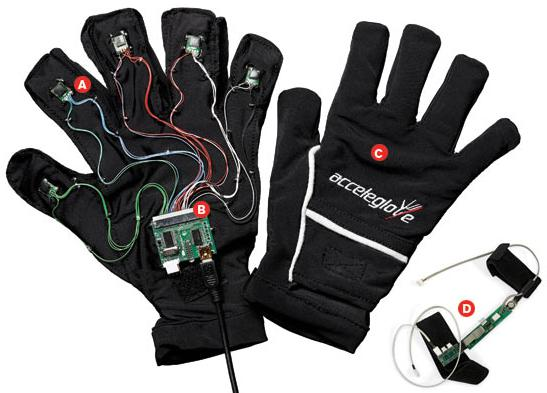
\includegraphics[scale=.25]{./Figures/Dataglove.jpg}}  \qquad
	{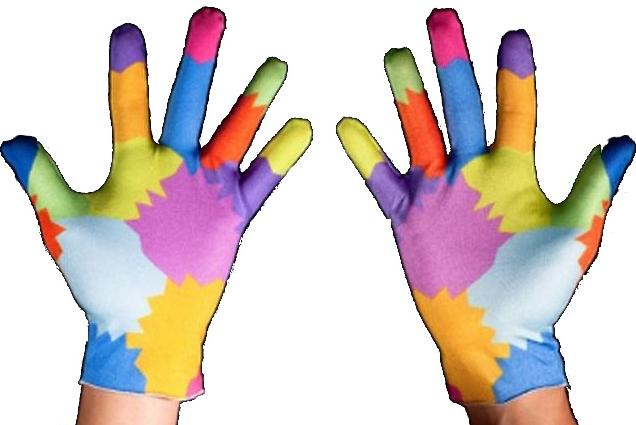
\includegraphics[scale=.25]{./Figures/colorGloves.jpg}} \qquad   	
	{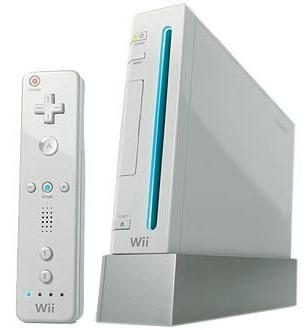
\includegraphics[scale=.29]{./Figures/wii.jpg}} 	  	
	\label{fig:Modelos:1}
}
\subfigure [Dispositivos basados en visión: en la imagen se observan distintos tipos de cámaras. A la izquierda de la imagen se observa una cámara web \protect\footnotemark{}, en el centro una cámara digital \protect\footnotemark{} y a la derecha de la imagen una cámara  TOF \protect\footnotemark{} .]
{
	{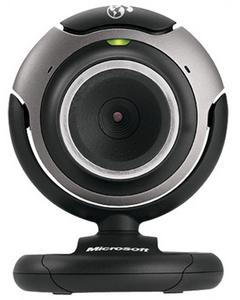
\includegraphics[scale=.3]{./Figures/webcam.jpg}} 		\qquad
	{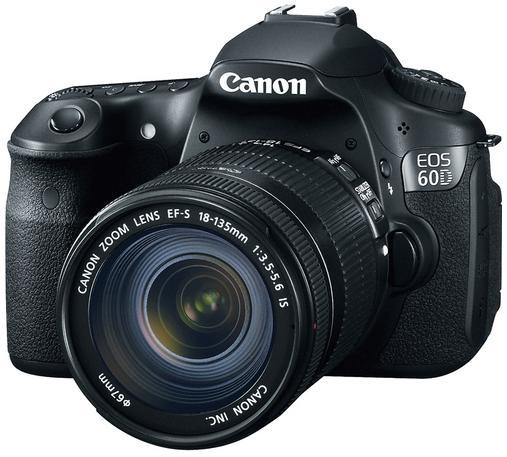
\includegraphics[scale=.2]{./Figures/digitalCamera.jpg}}  \qquad
	{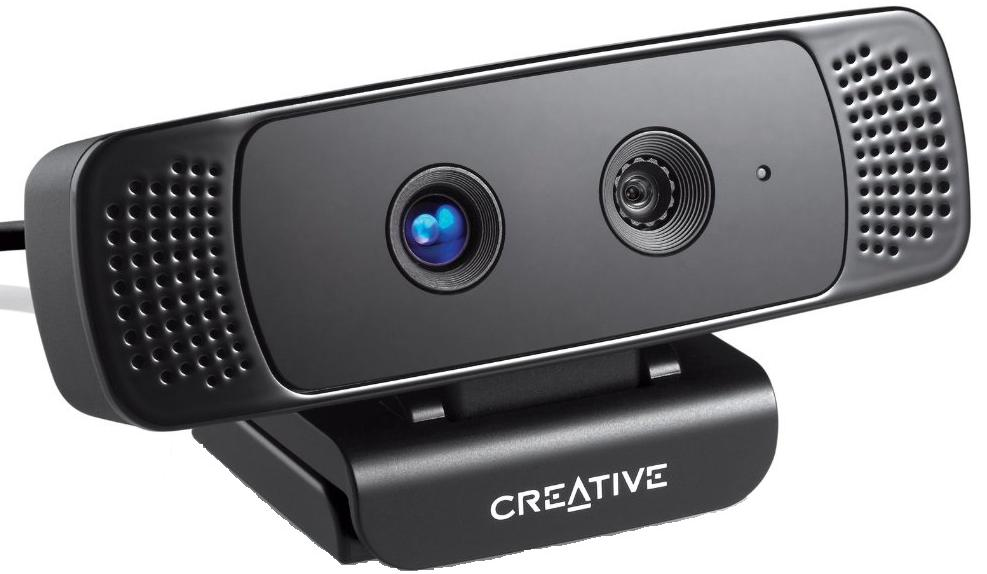
\includegraphics[scale=.15]{./Figures/TOF.jpg}} 
    \label{fig:Modelos:2} 
}
\caption{Dispositivos utilizados para la captura de gestos.} 
\label{fig:Modelos} 
\end{center}
\end{figure} 

En este trabajo, se toma el enfoque basado en la visión debido a que se busca obtener un sistema que para el usuario la interacción sea natural y la manera de lograrlo es tomando este enfoque.  

\footnotetext[1] {\url{ http://www.technologyreview.com/article/414021/open-source-data-glove/}} \stepcounter{footnote}
\footnotetext[2] {\url{http://www.digitaltrends.com/computing/the-gloves-that-could-change-the-world/}}
\footnotetext[3] {\url{https://www.nintendo.es/Wii/Wii-94559.html}}

\footnotetext[4] {\url{http://es.ccm.net/download/descargar-2562-driver-de-microsoft-lifecam-vx-3000}}
\footnotetext[5] {\url{http://www.canon.com.mx/ficha.aspx?id=722}} 
\footnotetext[6] {\url{http://us.creative.com/p/web-cameras/creative-senz3d}}


%::::::::::::::::::::::::::::::::::::::::::::::::::::::::::::::::::::::::::::::::::::::::::::::::::::::::::::::::::::::::::::::::::


\section{Estado del arte}\label{sec:EstadoDelArte} 

En esta sección se presentan los trabajos relevantes de cada uno de estos enfoques y también se mencionan algunos de los sistemas comerciales importantes. 

\subsection{Modelos de contacto}
 
Los primeros trabajos de reconocimiento de gestos con las manos utilizan este modelo, actualmente se sigue utilizando pero en menor grado. 

Un método de reconocimiento de gestos con las manos que utiliza guantes de datos \citep{Yoon2012} propone un sistema de reconocimiento de gestos estáticos, el cual reconoce $24$ gestos tomados del Lenguaje de Señas Americano, ASL (por sus siglas en inglés, American Sign Lenguaje). Este modelo consta de tres etapas. \\
La primera etapa del sistema consiste en capturar la información proporcionada por un guante de datos, la cual esta siendo enviada por un protocolo de control de transmisión TCP, (por sus siglas en inglés, Transmission Control Protocol).\\  
Una vez que la información es recibida, los datos son pre-procesados, es decir son normalizados y las características son extraídas, las características son las correlaciones que existe entre los ejes.\\     
La clasificación de gesto se realiza con un modelo de mezclas adaptativo. Para entrenar el modelo de mezclas se toman datos de $5$ personas, $300$ muestras de cada gestos, $8000$ por cada participante. Se realizaron pruebas con estos mismos datos; con un sujeto se alcanzó una precisión de $93.38 \%$ con los demás participantes se obtuvo una precisión de $89.97 \%$.\\  
La principal desventaja del sistema es que este requiere tiempo para adaptarse a distintos usuarios. Otra desventaja para este sistema es que solo reconoce gestos estáticos. 

A finales del año 2014 se lanzó el dispositivo MYO \footnote{\url{https://www.thalmic.com/en/myo/}}, el cual reconoce gestos dinámicos. Este aparato es un brazalete que reconoce $5$ gestos dinámicos. Leyendo la actividad de los músculos del antebrazo y mandando estas señales vía Bluetooth a la computadora donde estas señales son procesadas. \footnote{\url{http://www.digitaltrends.com/pc-accessory-reviews/myo-gesture-control-armband-review/}} 

No se cuenta con la informacion detallada del funcionamiento de MYO, lo único que se conoce es que el reconocimiento consta de tres etapas \footnote{\url{https://www.quora.com/How-does-MYO-wearable-gesture-control-work}}. La primera es la adquisición de la señales eléctricas que producen los músculos del antebrazo, las cuales son capturadas mediante sensores EMG (estos detectan la actividad eléctrica), giroscopio, acelerómetro y magnetómetro; en la segunda etapa se amplifica la señal y se aplica un filtro pasa banda. Por último se realiza el procesamiento de la señal donde se reconoce el gesto usando un algoritmo de aprendizaje de máquina desarrollado por la compañía.  

\begin{figure}[h!]
\begin{center}
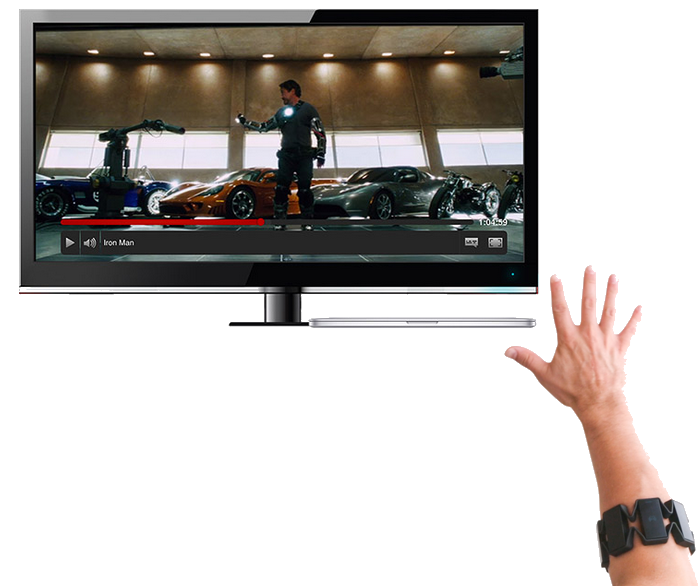
\includegraphics[scale=.5]{./Figures/MYO.png}
\end{center}
\caption{Ejemplo del reconocimiento del gesto usando MYO, controlando el volumen de la computadora. El dispositivo es el aparece en el brazo del sujeto. Imagen recuperada de \protect \footnotemark{}.}
\label{fig:Myo}
\end{figure}

\footnotetext{\url{https://www.myo.com/}} 

MYO funciona en cualquier ambiente donde haya variaciones en la iluminación y es invariante a rotación.\\ 
La principal desventaja es la calibración debido a que puede ser tediosa pues es necesario realizar un considerable número de repeticiones de algunos gestos.Otra desventaja es que tiene una cantidad considerable de falsos positivos \footnote{ \url{http://myogroupfive.blogspot.mx/2013/11/benefits-disadvantages-for-business\_ 24.html}}. Un punto importante es que para el uso del dispositivo es preferible el uso de manga corta. 


\subsection{Modelos basados en la visión}   

Este modelo es el más popular debido a la variedad de sus aplicaciones y la diversidad de cámaras existentes que proporcionan distinto tipo de información. Existe una gran gama de datos que se pueden extraer con este modelo, usando las técnicas o métodos adecuados para el tipo de datos extraído se puede llegar a tener gran precision en el reconocimiento. Enseguida se presenta tres trabajos relevantes los cuales utilizaron distintos tipos de cámaras y número de ellas. 

%En el trabajo propuesto por \cite{Premaratne2013} realizan un modelo de reconocimiento de gestos estático y dinámico basados en el algoritmo de Lucas-Kanade. Las principales ventajas de este método son que es invariante a rotación, escala y al fondo. Aunque el modelo es afectado por los cambios en la iluminación.
%::::::::::::::::::::::::::::::::::::::::::::::::::::::::::::::::::::::::::::::::::::::::::::::::::::::::

En trabajo de \citep{Huang2011}, propone un método que reconoce $11$ gestos estáticos y dinámicos. El sistema propuesto utiliza una cámara CCD para obtener la información de entrada. La aportación del trabajo es la segmentación de la mano que se lleva acabo usando filtros de Gabor. El sistema es robusto a la iluminación. 
 
Antes de hacer la segmentación de la mano se le aplica a la imagen un preprocesamiento que consiste en aplicar un filtro de Gabor. Después se escoge uno de los tres modelos del color; YCbCr, Gaussiano o Soriano, tomando en cuenta un nivel de gris.  
Una vez que es realizado el preprocesamiento el paso siguiente es segmentar de la imagen de la mano el antebrazo para esto se hace un barrido de la imagen por filas. Se segmenta la mano tomando en cuenta la distancia que existe entre la parte superior de la imagen y el número máximo de pixeles de un solo valor (el valor mayor del histograma).

Una vez realizada la segmentación se obtienen las características necesarias para el reconocimiento. Las características son obtenidas utilizando análisis de componentes principales, PCA (por sus siglas en inglés, Principal Component Analysis).\\
La clasificación se realiza por medio de maquinas de vectores de soporte, SVM (por sus siglas en inglés, Support Vector Machines).   

La precisión del reconocimiento varía dependiendo de las imágenes, si son reales o si se les aplica antes un filtro de Gabor. También cambia si el usuario usa manga corta o larga.  
Las principales ventajas son que el sistema funciona con cambios en la iluminación y es robusto a la rotación y escala. Una limitación de sistema es que el problema de oclusi\'on no es tratado. 

%:::::::::::::::::::::::::::::::::::::::::::::::::::::::::::::::::::::::::::::::::::::::::::

Otro trabajo propuesto \citep{Caputo2012} realiza el reconocimiento de  gestos dinámicos y estáticos, estos últimos son utilizados para determinar el inicio y el término de los gestos dinámicos. Se utilizan dos sensores Kinect y una cámara web Logitech C910 de alta definición para capturar los gestos. El trabajo está compuesto de cuatro etapas.\\
La primera es la configuración de los dispositivos de captura de datos del sistema. Los dos sensores Kinect son calibrados entre ellos para generar un sistema de coordenadas que esta basado en la ubicación de la  manos y la cabeza. La cámara y los dispositivos Kinect no son sincronizados entre si.  

La parte de la detección y seguimiento  se lleva acabo utilizando la librería OPENNI, en específico usando la detección del esqueleto. El esqueleto nos proporciona el punto de la palma de la mano por la cual la región de interés, ROI (por sus siglas en inglés, Region of Interest) es seleccionada. Para tener una  mejor aproximación de la localización de la mano, se utiliza la cámara RGB. La localización de la mano se realiza convirtiendo la imagen en una imagen binaria, usando un umbral que es determinado por el espacio del color HSV (Matiz, Saturación, Valor); son utilizados guantes neón color rosa o verde para ubicar con mayor facilidad las manos.   

Una vez obtenida la imagen binaria se calcula el contorno de la mano usando el algoritmo de Chang y Chen, dicho contorno es extraído como polígono y  es simplificado con el algoritmo de Douglas Peuker. 

El reconocimiento del gesto utiliza el empatamiento de polígonos, el cual se basa en comparar dos polígonos, mediante distancias. Esto usando Distancia de momentos HU (Hu-moments distance) y ángulo de giro (turning angle). 
Los gestos 3D son calculados usando la diferencia de las posiciones de la mano en cada cuadro. Las fórmulas para calcular estos gestos depende de que gesto se  realice.  
Para probar la precisión del sistema se crearon dos bases de datos: una con $120$ polígonos etiquetados que representan $11$ gestos y otra con $144$ gestos de $3$ personas distintas realizando los $11$ gestos. La precisión obtenida usando la distancia de ángulo de giro es de $85 \%$, usando la distancia de momentos HU la precisión es de $58 \%$.  

%::::::::::::::::::::::::::::::::::::::::::::::::::::::::::::::::::::::::::::::::::::::::::::::::::::::::

Otra aportación importante fue hecha por \citep{Kang2013} ellos proponen un sistema de reconocimiento de  gestos estáticos utilizando el sensor Kinect como dispositivo de captura de los gestos. El sistema reconoce $24$ gestos, los cuales pertenecen al ASL, el reconocimiento es realizado en cuatro etapas, las cuales se explican a continuación.  

En la primera etapa la imagen es capturada y la mano junto con el antebrazo son segmentados del fondo. Las imágenes de entrada del sistema son proporcionadas por el sensor de profundidad del Kinect, la mano es detectada usando el SDK (Software Developmet Kit) del Kinect, que proporciona el punto de la palma de la mano, la región de interés es seleccionada usando este punto, donde  solo se encuentra la mano y parte del antebrazo.   

Después se extraen las características, las cuales son extraídas usando Histogramas Orientados a Gradientes, HOG (Histogram of Oriented Gredient).  

Para la clasificación de los gestos, se utiliza el algoritmo de aprendizaje de máquina, máquinas de soporte vectorial.\\
Para el entrenamiento se utilizaron $2400$ imágenes, $100$ por cada letra del alfabeto. Se encontró que existe gesto ambiguos, es decir que no se pueden clasificar correctamente, estos son los gestos que representan la letras A, E, M, N, S, T. 
Se realizo una prueba en linea, donde los gestos aparecían aleatoriamente para ser clasificados. La precisión de todos los gestos se encuentra alrededor de $92.8 \%$, pero el de los gestos ambiguos es $72.9 \%$\\
Por ultimo una interfaz gráfica es mostrada donde se aprecia el reconocimiento de los gestos en tiempo real.  

%::::::::::::::::::::::::::::::::::::::::::::::::::::::::::::::::::::::::::::::::::::::::::::::

%La SECCIÓN A pesar que la mayoría de los modelos vistos en la parte de arriba solucionan muchos de los problemas de los modelos basados en la visi\'on. Ninguno de ellos puede resolver el problema de iluminaci\'on y oclusi\'on, formada por lo dedos. All\'i la importancia de la investigaci\'on propuesta, pues dar\'a soluci\'on a estos inconvenientes al momento de reconocer los gestos.
 
\subsection{Sistemas comerciales}

Existen dispositivos como: Leap Motion \footnote{\label{LeapMotionFN} \url{https://www.leapmotion.com/}}, MYO \footnote{\label{MyoFN}  \url{https://www.myo.com/}}, y software como: Flutter \footnote{\label{FlutterFN} \url{ https://flutterapp.com/}}, que realizan el reconocimiento de gestos, y este reconocimiento es aplicado para controlar la computadora. Algunos de estos dispositivos comerciales tienen  buen rendimiento en cuanto a la precisión y a sobrellevar los problemas del reconocimiento de gestos. El inconveniente es que los desarrolladores de los dispositivos o software no dan a conocer los detalles de como solucionan algunos de los problemas o como mejoran la precisión. \\ 
Enseguida se describen los sistemas mencionados anteriormente.
 
El dispositivo Leap Motion (figura \ref{fig:LeapMotion}) fue creado para el seguimiento de manos y dedos. Este también hace el reconocimiento de ciertos gestos estáticos y dinámicos. El dispositivo consta de tres emisores y dos cámaras infrarrojas, estos sensores capturan los datos crudos en un rango de $60 \times 60 \times 60$ $cm.$ y con la información capturada se construye un modelo 3D de las manos \citep{Weichert2013}. 

\begin{figure}[h!]
\begin{center}
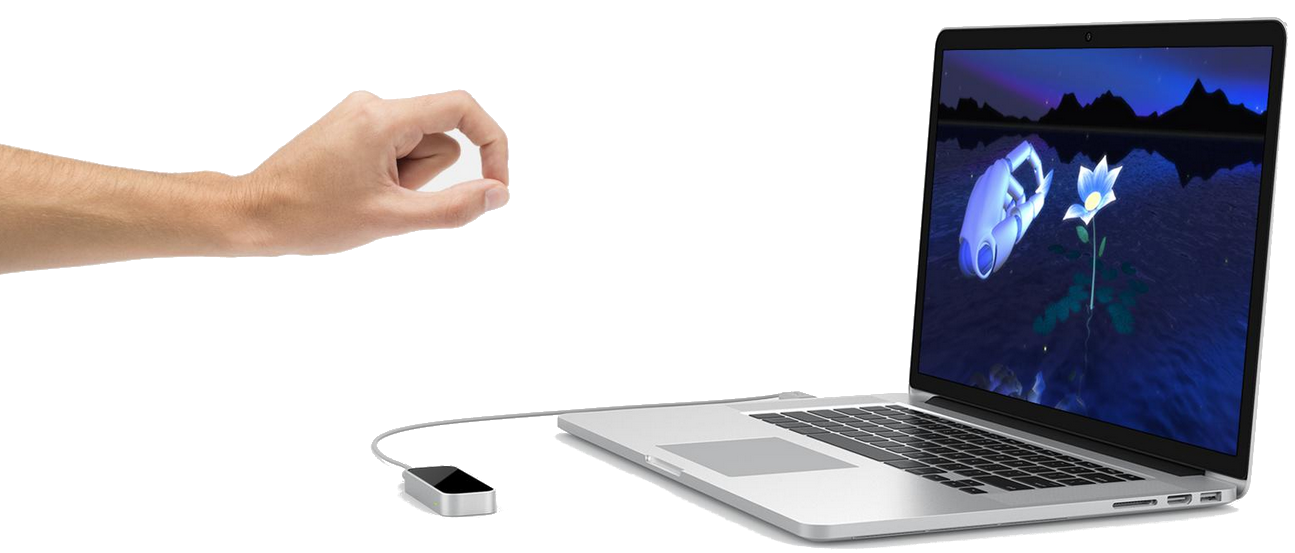
\includegraphics[scale=.3]{./Figures/LeapMotion.png}
\end{center}
\caption{Ejemplo del reconocimiento del gesto usando Leap Motion, mostrando mediante una aplicación donde los gestos son representados en 3D, que es el dispositivo que se encuentra conectado a la Laptop. Imagen recuperada de \ref{LeapMotionFN}.}
\label{fig:LeapMotion}
\end{figure}

El proceso de captura de los datos, la segmentación, la extracción de características, el seguimiento y el reconocimiento del dispositivo no se conoce a detalle, pues no ha sido publicado.\\ 
Solo se conoce \footnote{ \url{http://blog.leapmotion.com/hardware-to-software-how-does-the-leap-motion-controller-work/}} que se utilizan tres cámaras infrarrojas, con la imágenes obtenidas con se hace una representación 3D de las manos, antes de realizar el modelo las imágenes son segmentadas del fondo para eliminar el ruido generado por la iluminación u otros objetos que causen ruido en la imágenes. \\
Para realizar el seguimiento se extraen la características. Una de ellas son el dedos, el algoritmo de seguimiento interpreta la información 3D e infiere la posición de los objetos ocluidos. Se aplican filtros para suavizar los datos. 


Enseguida se explica el software de reconocimiento de gestos estáticos Flutter, fig:\ref{fig:Flutter} el cual reconoce cuatro gestos estáticos usando la cámara web como dispositivo de entrada. 

Se desconoce como funciona el software, solo se sabe que la mano es detectada por la cámara, para que la detección sea correcta la mano tiene que estar totalmente frente a la cámara web. Los algoritmos utilizados para el reconocimiento no se conocen.  
\begin{figure}[h!]
\begin{center}
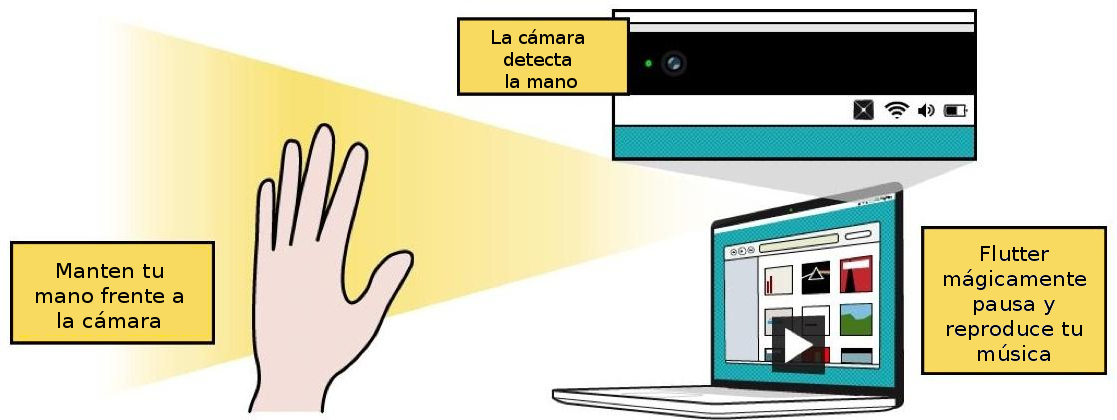
\includegraphics[scale=.4]{./Figures/Flutter.jpg}
\end{center}
\caption{La imagen anterior representa el funcionamiento del software Flutter. Imagen recuperada de \ref{FlutterFN} .}
\label{fig:Flutter}
\end{figure}

Flutter permite controlar aplicaciones multimedia como: YouTube \footnote{\url{https://www.youtube.com/}} ,VLC \footnote{\url{http://www.videolan.org/vlc/}}, Spotify \footnote{\url{https://www.spotify.com/}}, Netflix \footnote{\url{https://www.netflix.com/}}. Las limitaciones del software son que solo reconoce gestos estáticos. Una desventaja es que presenta falsos positivos al reconocer acciones del usuario.  

%::::::::::::::::::::::::::::::::::::::::::::::::::::::::::::::::::::::::::::::::::::::::::::::::::::::::: 

Aunque estos dispositivos y software para reconocer gestos solucionan algunos problemas importantes en el área, sigue existiendo el problema de bloqueo e iluminación.
De allí la importancia que existan nuevos modelos que ataquen estos problemas que se presentan frecuentemente en el reconocimiento de los gestos.
  
\section{Organizaci\'on de la tesis}\label{OrganizacionTesis}

La tesis se encuentra distribuida de la siguiente manera: la segunda sección presenta los fundamentos teóricos como base para la comprensión del tema. La tercera sección presenta la metodología utiliza en el sistema propuesto. En la cuarta sección se encuentran los detalles de la implementación del sistema. En la quinta sección están las pruebas realizadas al sistema junto con los resultados y las discusiones de estos. Finalmente la sexta sección presenta las conclusiones generales del sistema y el trabajo futuro. 

} }%
%BeginExpansion
\chapter{Introducci\'on}\label{capit:cap1}
\vspace{-2.0325ex}%
\noindent
\rule{\textwidth}{0.5pt}
\vspace{-5.5ex}% 
\newcommand{\pushline}{\Indp}% Indent puede ir o no :p

La interacción entre humanos se lleva a cabo gracias a la comunicación  que existe entre ellos, esta puede ser oral o escrita y generalmente viene acompañada de gestos realizados con la cara, manos o otra cualquier parte del cuerpo. 
Estos gestos sirven como complemento de la comunicación pues ayudan a que el mensaje sea percibido de manera correcta.

El creciente desarrollo de la tecnología en especial el desarrollo de computadoras, su incremento en procesamiento, la reducción de su tamaño y costos ha hecho que estas se incorporen cada vez más y sean parte esencial en nuestra vida diaria. De manera que se han creado y con ello estudiado distintas áreas de las ciencias computacionales, particularmente el área de interacción humano computadora (HCI, por sus siglas en ingl\'es Human Computer Interaction), el área encargada del estudio y diseño de la forma en que el humano interactua con la computadora. 
Uno de los objetivos principales de esta área es que la interacción se lleve acabo de manera natural. 
La manera en que el humano interactua con la computadora ha sido básicamente la misma desde que se empezó a tener acceso a ellas, fue hasta principios de esta década cuando la interacción ha empezado a cambiar pues ahora existen pantallas táctiles, reconocimiento de voz. Estas formas de interacción has sido aceptadas por los usuarios ya que hacen que la forma en que nos ``comuniquemos'' con la computadora sea fácil y sencilla. No resulta extraño que los investigadores de HCI se hayan interesado en los gestos corporales, en especial los gestos realizados con las manos, para crear un ambiente natural entre el usuario y la computadora.  
Por lo que es necesario que la computadora pueda identificar la o las manos del usuario y reconocer el gesto que este realiza. 

A finales de los años noventa se empezar\'on a desarrollar t\'ecnicas para  el reconocimiento de gestos con las manos. Los primeros enfoques utilizaban como medio de captura sensores como: guantes de datos, marcadores de colores y acelerómetros; los cuales se colocaban en la o las manos para poder capturar la posición e identificar la pose realizada. 
Las técnicas desarrolladas posteriormente obtienen la información necesaria para reconocer el gesto usando distintos tipos de imágenes o vídeos, que son obtenidos mediante diversos tipos de cámaras, por lo que no es necesario vestir algún dispositivo para reconocer un gesto hecho con las manos.

Los métodos que utilizan imágenes o vídeo son los más utilizados para realizar el reconocimiento de los gestos ya que la interacción entre el usuario y la computadora es más natural, el inconveniente con estos métodos es que es un problema difícil de resolver pues existen diversos aspectos que hay que tener en cuenta para obtener una buena precisión en el reconocimiento del gesto; por ejemplo tener en cuenta la resolución del dispositivo de captura, el ruido que existe en las imágenes, el tiempo de computo para realizar el procesamiento de las imágenes y las situaciones que se pueden presentar en la vida diaria que puedan entorpecer el reconocimiento del gesto. 

Aunque existe una gran variedad de métodos y sistemas que hacen el reconocimiento de gestos de las manos no existe alguno que presente en el reconocimiento un alto grado de precisión en todas las situaciones que se presentan en el mundo real, tales como; condiciones diversas de iluminación ya sea baja o alta, que funcionen en tiempo real, que funcionen a diversas escalas, es decir no importando el tamaño de la mano, que sea invariante a rotación, invariante al color de la piel y cuando exista algún bloque parcial en el área de la mano.\\
Es por eso que se propone crear un sistema que reconozca gestos realizados con las manos, en situaciones que presentan baja iluminación y cuando existe oclusión de los dedos. 
El sistema se enfoca en atacar estos problemas cuando las manos no se encuentran en movimiento, pero también se abordar\'an los gestos con las manos que involucran movimiento. El objetivo del sistema es mostrar que en ciertas ocasiones es posible obtener mayor precisión en el reconocimiento de los gestos utilizando como medio de captura dos sensores Kinect.   


%::::::::::::::::::::::::::::::::::::::::::::::::::::::::::::::::::::::::::::::::::::::::::::::::::::::::::::::::::::::::::::::::::


\section{Definici\'on del problema}\label{sec:DefinicionProblema}

Existen diversas técnicas que logran obtener buena precisión en el reconocimiento de gestos realizados con las manos.Sin embargo no hay técnicas que tengan buena precisión y que al mismo tiempo se adecuen a todo tipo de situaciones que se presentan en la vida real como: amigable con el usuario, invariante a la iluminación, rotación, al fondo, que funcione en tiempo real o cuando exista oclusión.


%:::::::::::::::::::::::::::::::::::::::::::::::::::::::::::::::::::::::::::::::::::::::::::::::::::::::::::::::::::::::::::

\section{Justificaci\'on}\label{sec:Just}

Los métodos de reconocimiento de gestos desarrollados logran obtener un buen grado de reconocimiento en ciertas situaciones, generalmente en situaciones controladas.
De manera que se necesitan nuevos métodos que funcione no solamente en condiciones ideales si no en situaciones que se presentan en la vida diaria y al mismo tiempo se obtenga un alto grado de precisión.  

Una vez logrado lo anterior se pueden desarrollar nuevas aplicaciones y tecnologías que ayuden a interactuar con naturalidad al usuario y la computadora.


%:::::::::::::::::::::::::::::::::::::::::::::::::::::::::::::::::::::::::::::::::::::::::::::::::::::::::::::::::::::::::::::::


\section{Objetivo general}\label{sec:ObjetivoGeneral}
 
Desarrollar un sistema de reconocimiento de gestos con las manos, gestos estáticos y dinámicos. El sistema debe funcionar ciertas situaciones que se presentan en un ambiente natural. Es decir el sistema debe  funcionar en circunstancias de baja iluminación y cuando exista obstrucción causada por los dedos en gestos dinámicos.


%:::::::::::::::::::::::::::::::::::::::::::::::::::::::::::::::::::::::::::::::::::::::::::::::::::::::::::::::::::::::::::::::


\section{Objetivos espec\'ificos}\label{sec:objetivosEspecificos}

\begin{itemize}
	\item Identificar los m\'etodos actuales de reconocimiento de gestos, estáticos y din\'amicos cuando existe baja iluminación  y cuando existe oclusión. 
	
	\item  Obtener conocimiento acerca del funcionamiento de sistema Microsoft Kinect.
	
	\item Desarrollar un sistema de reconocimiento de gestos estáticos y dinámicos, fusionando la información de los sensores de  profundidad de dos dispositivos kinect. El sistema desarrollado deberá funcionar en circunstancias de baja iluminación y también cuando existe oclusión, causada por los dedos. 
	
	\item Validar el sistema dise\~nado, en cuanto a su eficiencia presentada en base al reconocimiento de los gestos, en circunstancias de baja iluminación y oclusión. En el análisis del sistema se usar\'a información real.  
	
	\item Comparar y validar el modelo propuesto haciendo uso de uno y dos dispositivos Kinect. 
\end{itemize}


%::::::::::::::::::::::::::::::::::::::::::::::::::::::::::::::::::::::::::::::::::::::::::::::::::::::::::::::::::::::::::::::::::


\section{Limitaciones y suposiciones}\label{sec:Limitaciones&Suposiciones}

Gran porcentaje de los trabajos previos en el \'area de reconocimiento de gestos con las manos basados en el modelo de la visión  utilizan c\'amaras digitales o c\'amaras web. Esta investigación utiliza dos dispositivos Kinect, para obtener la información de entrada del sistema.

De  manera que las limitaciones del sistema propuesto están dadas por las características de dicho dispositivo, tales como la distancia  a la que se encuentran los dispositivos con el usuario y la resolución del sensor. 

Otra limitante es el número de gestos que podrá reconocer el sistema.


%::::::::::::::::::::::::::::::::::::::::::::::::::::::::::::::::::::::::::::::::::::::::::::::::::::::::::::::::::::::::::::::::::


\section{Reconocimiento de gestos con la manos}\label{sec:ReconocimientoGestos} 

Los gestos están definidos como movimientos del cuerpo expresivos y significativos que involucran a los dedos, manos, brazos, cabeza, cara o cuerpo con la intención de transmitir información relevante o de interactuar con el ambiente, \citep{Mitra2007}.

Los primeros enfoques para llevar acabo el reconocimiento de gestos con las manos fue usando modelos de contacto \citep{Rautaray2012} y \citep{Nayakwadi2014}.\\
El modelo utiliza dispositivos que est\'an en contacto f\'isico con la mano del usuario \ref{fig:Modelos:1} para reconocer el gesto. Por ejemplo usan guantes de datos, marcadores de colores, acelerómetros y pantallas multi-touch. Este enfoque no es  tan aceptado pues entorpecen la naturalidad entre la interacción del humano y la computadora.\\
Los modelos basados en la visión \ref{fig:Modelos:2} surgieron como respuesta a esta desventaja. Estos utilizan cámaras para extraer la información necesaria para realizar el reconocimiento. Los dispositivos van desde cámaras web hasta algunas más sofisticadas por ejemplo c\'amaras de profundidad.   

\begin{figure}[h!]
\begin{center}
\subfigure [Dispositivos basados en contacto: a la izquierda de la imagen se observan los guantes de datos \protect\footnotemark{}
, en el centro los guantes de colores  \protect\footnotemark{}  y a la derecha se encuentra el dispositivo wii \protect\footnotemark{} . \addtocounter{footnote}{-3}]
{
    {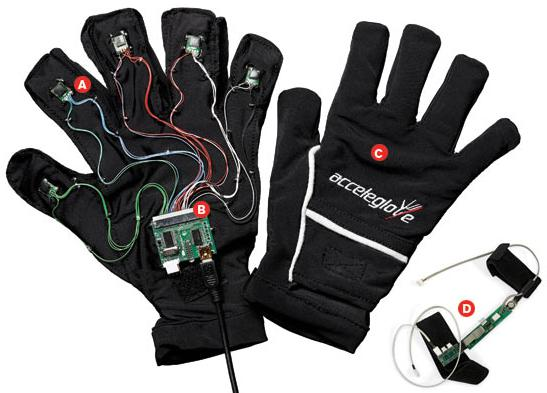
\includegraphics[scale=.25]{./Figures/Dataglove.jpg}}  \qquad
	{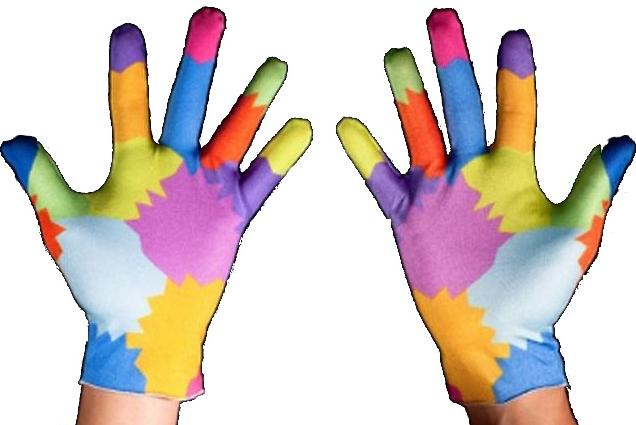
\includegraphics[scale=.25]{./Figures/colorGloves.jpg}} \qquad   	
	{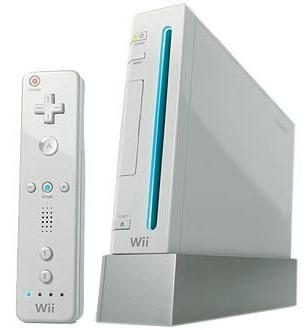
\includegraphics[scale=.29]{./Figures/wii.jpg}} 	  	
	\label{fig:Modelos:1}
}
\subfigure [Dispositivos basados en visión: en la imagen se observan distintos tipos de cámaras. A la izquierda de la imagen se observa una cámara web \protect\footnotemark{}, en el centro una cámara digital \protect\footnotemark{} y a la derecha de la imagen una cámara  TOF \protect\footnotemark{} .]
{
	{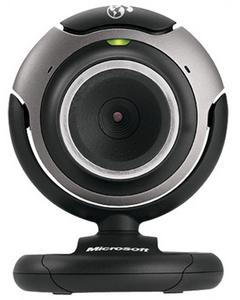
\includegraphics[scale=.3]{./Figures/webcam.jpg}} 		\qquad
	{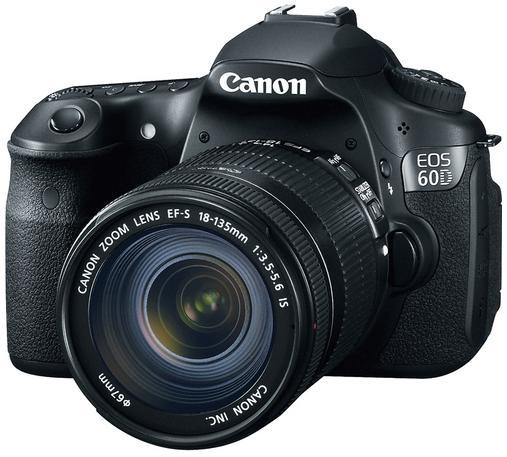
\includegraphics[scale=.2]{./Figures/digitalCamera.jpg}}  \qquad
	{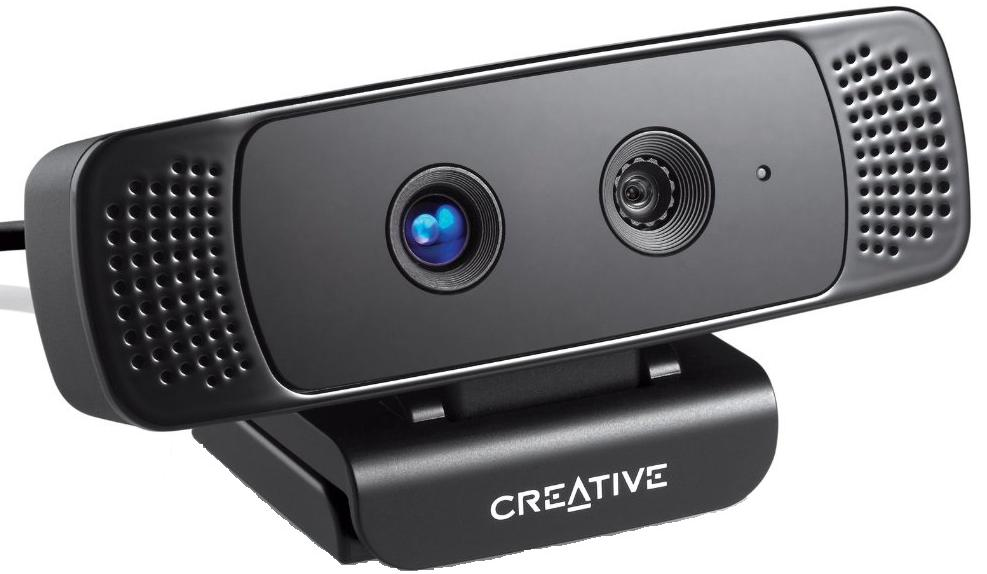
\includegraphics[scale=.15]{./Figures/TOF.jpg}} 
    \label{fig:Modelos:2} 
}
\caption{Dispositivos utilizados para la captura de gestos.} 
\label{fig:Modelos} 
\end{center}
\end{figure} 

En este trabajo, se toma el enfoque basado en la visión debido a que se busca obtener un sistema que para el usuario la interacción sea natural y la manera de lograrlo es tomando este enfoque.  

\footnotetext[1] {\url{ http://www.technologyreview.com/article/414021/open-source-data-glove/}} \stepcounter{footnote}
\footnotetext[2] {\url{http://www.digitaltrends.com/computing/the-gloves-that-could-change-the-world/}}
\footnotetext[3] {\url{https://www.nintendo.es/Wii/Wii-94559.html}}

\footnotetext[4] {\url{http://es.ccm.net/download/descargar-2562-driver-de-microsoft-lifecam-vx-3000}}
\footnotetext[5] {\url{http://www.canon.com.mx/ficha.aspx?id=722}} 
\footnotetext[6] {\url{http://us.creative.com/p/web-cameras/creative-senz3d}}


%::::::::::::::::::::::::::::::::::::::::::::::::::::::::::::::::::::::::::::::::::::::::::::::::::::::::::::::::::::::::::::::::::


\section{Estado del arte}\label{sec:EstadoDelArte} 

En esta sección se presentan los trabajos relevantes de cada uno de estos enfoques y también se mencionan algunos de los sistemas comerciales importantes. 

\subsection{Modelos de contacto}
 
Los primeros trabajos de reconocimiento de gestos con las manos utilizan este modelo, actualmente se sigue utilizando pero en menor grado. 

Un método de reconocimiento de gestos con las manos que utiliza guantes de datos \citep{Yoon2012} propone un sistema de reconocimiento de gestos estáticos, el cual reconoce $24$ gestos tomados del Lenguaje de Señas Americano, ASL (por sus siglas en inglés, American Sign Lenguaje). Este modelo consta de tres etapas. \\
La primera etapa del sistema consiste en capturar la información proporcionada por un guante de datos, la cual esta siendo enviada por un protocolo de control de transmisión TCP, (por sus siglas en inglés, Transmission Control Protocol).\\  
Una vez que la información es recibida, los datos son pre-procesados, es decir son normalizados y las características son extraídas, las características son las correlaciones que existe entre los ejes.\\     
La clasificación de gesto se realiza con un modelo de mezclas adaptativo. Para entrenar el modelo de mezclas se toman datos de $5$ personas, $300$ muestras de cada gestos, $8000$ por cada participante. Se realizaron pruebas con estos mismos datos; con un sujeto se alcanzó una precisión de $93.38 \%$ con los demás participantes se obtuvo una precisión de $89.97 \%$.\\  
La principal desventaja del sistema es que este requiere tiempo para adaptarse a distintos usuarios. Otra desventaja para este sistema es que solo reconoce gestos estáticos. 

A finales del año 2014 se lanzó el dispositivo MYO \footnote{\url{https://www.thalmic.com/en/myo/}}, el cual reconoce gestos dinámicos. Este aparato es un brazalete que reconoce $5$ gestos dinámicos. Leyendo la actividad de los músculos del antebrazo y mandando estas señales vía Bluetooth a la computadora donde estas señales son procesadas. \footnote{\url{http://www.digitaltrends.com/pc-accessory-reviews/myo-gesture-control-armband-review/}} 

No se cuenta con la informacion detallada del funcionamiento de MYO, lo único que se conoce es que el reconocimiento consta de tres etapas \footnote{\url{https://www.quora.com/How-does-MYO-wearable-gesture-control-work}}. La primera es la adquisición de la señales eléctricas que producen los músculos del antebrazo, las cuales son capturadas mediante sensores EMG (estos detectan la actividad eléctrica), giroscopio, acelerómetro y magnetómetro; en la segunda etapa se amplifica la señal y se aplica un filtro pasa banda. Por último se realiza el procesamiento de la señal donde se reconoce el gesto usando un algoritmo de aprendizaje de máquina desarrollado por la compañía.  

\begin{figure}[h!]
\begin{center}
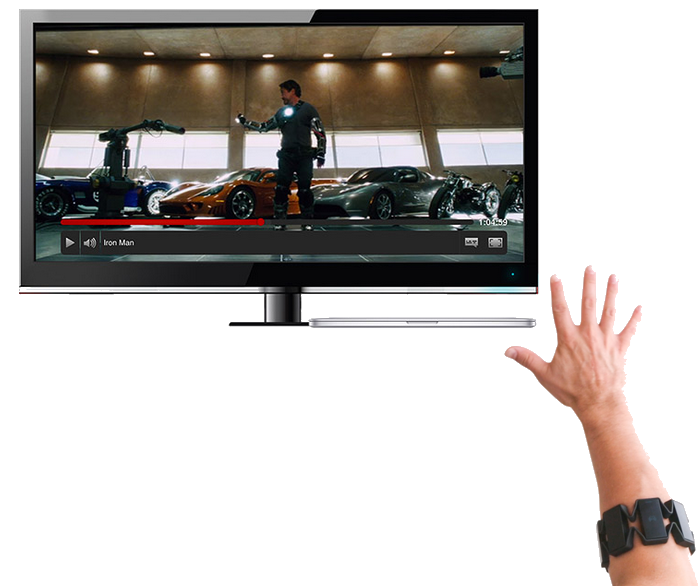
\includegraphics[scale=.5]{./Figures/MYO.png}
\end{center}
\caption{Ejemplo del reconocimiento del gesto usando MYO, controlando el volumen de la computadora. El dispositivo es el aparece en el brazo del sujeto. Imagen recuperada de \protect \footnotemark{}.}
\label{fig:Myo}
\end{figure}

\footnotetext{\url{https://www.myo.com/}} 

MYO funciona en cualquier ambiente donde haya variaciones en la iluminación y es invariante a rotación.\\ 
La principal desventaja es la calibración debido a que puede ser tediosa pues es necesario realizar un considerable número de repeticiones de algunos gestos.Otra desventaja es que tiene una cantidad considerable de falsos positivos \footnote{ \url{http://myogroupfive.blogspot.mx/2013/11/benefits-disadvantages-for-business\_ 24.html}}. Un punto importante es que para el uso del dispositivo es preferible el uso de manga corta. 


\subsection{Modelos basados en la visión}   

Este modelo es el más popular debido a la variedad de sus aplicaciones y la diversidad de cámaras existentes que proporcionan distinto tipo de información. Existe una gran gama de datos que se pueden extraer con este modelo, usando las técnicas o métodos adecuados para el tipo de datos extraído se puede llegar a tener gran precision en el reconocimiento. Enseguida se presenta tres trabajos relevantes los cuales utilizaron distintos tipos de cámaras y número de ellas. 

%En el trabajo propuesto por \cite{Premaratne2013} realizan un modelo de reconocimiento de gestos estático y dinámico basados en el algoritmo de Lucas-Kanade. Las principales ventajas de este método son que es invariante a rotación, escala y al fondo. Aunque el modelo es afectado por los cambios en la iluminación.
%::::::::::::::::::::::::::::::::::::::::::::::::::::::::::::::::::::::::::::::::::::::::::::::::::::::::

En trabajo de \citep{Huang2011}, propone un método que reconoce $11$ gestos estáticos y dinámicos. El sistema propuesto utiliza una cámara CCD para obtener la información de entrada. La aportación del trabajo es la segmentación de la mano que se lleva acabo usando filtros de Gabor. El sistema es robusto a la iluminación. 
 
Antes de hacer la segmentación de la mano se le aplica a la imagen un preprocesamiento que consiste en aplicar un filtro de Gabor. Después se escoge uno de los tres modelos del color; YCbCr, Gaussiano o Soriano, tomando en cuenta un nivel de gris.  
Una vez que es realizado el preprocesamiento el paso siguiente es segmentar de la imagen de la mano el antebrazo para esto se hace un barrido de la imagen por filas. Se segmenta la mano tomando en cuenta la distancia que existe entre la parte superior de la imagen y el número máximo de pixeles de un solo valor (el valor mayor del histograma).

Una vez realizada la segmentación se obtienen las características necesarias para el reconocimiento. Las características son obtenidas utilizando análisis de componentes principales, PCA (por sus siglas en inglés, Principal Component Analysis).\\
La clasificación se realiza por medio de maquinas de vectores de soporte, SVM (por sus siglas en inglés, Support Vector Machines).   

La precisión del reconocimiento varía dependiendo de las imágenes, si son reales o si se les aplica antes un filtro de Gabor. También cambia si el usuario usa manga corta o larga.  
Las principales ventajas son que el sistema funciona con cambios en la iluminación y es robusto a la rotación y escala. Una limitación de sistema es que el problema de oclusi\'on no es tratado. 

%:::::::::::::::::::::::::::::::::::::::::::::::::::::::::::::::::::::::::::::::::::::::::::

Otro trabajo propuesto \citep{Caputo2012} realiza el reconocimiento de  gestos dinámicos y estáticos, estos últimos son utilizados para determinar el inicio y el término de los gestos dinámicos. Se utilizan dos sensores Kinect y una cámara web Logitech C910 de alta definición para capturar los gestos. El trabajo está compuesto de cuatro etapas.\\
La primera es la configuración de los dispositivos de captura de datos del sistema. Los dos sensores Kinect son calibrados entre ellos para generar un sistema de coordenadas que esta basado en la ubicación de la  manos y la cabeza. La cámara y los dispositivos Kinect no son sincronizados entre si.  

La parte de la detección y seguimiento  se lleva acabo utilizando la librería OPENNI, en específico usando la detección del esqueleto. El esqueleto nos proporciona el punto de la palma de la mano por la cual la región de interés, ROI (por sus siglas en inglés, Region of Interest) es seleccionada. Para tener una  mejor aproximación de la localización de la mano, se utiliza la cámara RGB. La localización de la mano se realiza convirtiendo la imagen en una imagen binaria, usando un umbral que es determinado por el espacio del color HSV (Matiz, Saturación, Valor); son utilizados guantes neón color rosa o verde para ubicar con mayor facilidad las manos.   

Una vez obtenida la imagen binaria se calcula el contorno de la mano usando el algoritmo de Chang y Chen, dicho contorno es extraído como polígono y  es simplificado con el algoritmo de Douglas Peuker. 

El reconocimiento del gesto utiliza el empatamiento de polígonos, el cual se basa en comparar dos polígonos, mediante distancias. Esto usando Distancia de momentos HU (Hu-moments distance) y ángulo de giro (turning angle). 
Los gestos 3D son calculados usando la diferencia de las posiciones de la mano en cada cuadro. Las fórmulas para calcular estos gestos depende de que gesto se  realice.  
Para probar la precisión del sistema se crearon dos bases de datos: una con $120$ polígonos etiquetados que representan $11$ gestos y otra con $144$ gestos de $3$ personas distintas realizando los $11$ gestos. La precisión obtenida usando la distancia de ángulo de giro es de $85 \%$, usando la distancia de momentos HU la precisión es de $58 \%$.  

%::::::::::::::::::::::::::::::::::::::::::::::::::::::::::::::::::::::::::::::::::::::::::::::::::::::::

Otra aportación importante fue hecha por \citep{Kang2013} ellos proponen un sistema de reconocimiento de  gestos estáticos utilizando el sensor Kinect como dispositivo de captura de los gestos. El sistema reconoce $24$ gestos, los cuales pertenecen al ASL, el reconocimiento es realizado en cuatro etapas, las cuales se explican a continuación.  

En la primera etapa la imagen es capturada y la mano junto con el antebrazo son segmentados del fondo. Las imágenes de entrada del sistema son proporcionadas por el sensor de profundidad del Kinect, la mano es detectada usando el SDK (Software Developmet Kit) del Kinect, que proporciona el punto de la palma de la mano, la región de interés es seleccionada usando este punto, donde  solo se encuentra la mano y parte del antebrazo.   

Después se extraen las características, las cuales son extraídas usando Histogramas Orientados a Gradientes, HOG (Histogram of Oriented Gredient).  

Para la clasificación de los gestos, se utiliza el algoritmo de aprendizaje de máquina, máquinas de soporte vectorial.\\
Para el entrenamiento se utilizaron $2400$ imágenes, $100$ por cada letra del alfabeto. Se encontró que existe gesto ambiguos, es decir que no se pueden clasificar correctamente, estos son los gestos que representan la letras A, E, M, N, S, T. 
Se realizo una prueba en linea, donde los gestos aparecían aleatoriamente para ser clasificados. La precisión de todos los gestos se encuentra alrededor de $92.8 \%$, pero el de los gestos ambiguos es $72.9 \%$\\
Por ultimo una interfaz gráfica es mostrada donde se aprecia el reconocimiento de los gestos en tiempo real.  

%::::::::::::::::::::::::::::::::::::::::::::::::::::::::::::::::::::::::::::::::::::::::::::::

%La SECCIÓN A pesar que la mayoría de los modelos vistos en la parte de arriba solucionan muchos de los problemas de los modelos basados en la visi\'on. Ninguno de ellos puede resolver el problema de iluminaci\'on y oclusi\'on, formada por lo dedos. All\'i la importancia de la investigaci\'on propuesta, pues dar\'a soluci\'on a estos inconvenientes al momento de reconocer los gestos.
 
\subsection{Sistemas comerciales}

Existen dispositivos como: Leap Motion \footnote{\label{LeapMotionFN} \url{https://www.leapmotion.com/}}, MYO \footnote{\label{MyoFN}  \url{https://www.myo.com/}}, y software como: Flutter \footnote{\label{FlutterFN} \url{ https://flutterapp.com/}}, que realizan el reconocimiento de gestos, y este reconocimiento es aplicado para controlar la computadora. Algunos de estos dispositivos comerciales tienen  buen rendimiento en cuanto a la precisión y a sobrellevar los problemas del reconocimiento de gestos. El inconveniente es que los desarrolladores de los dispositivos o software no dan a conocer los detalles de como solucionan algunos de los problemas o como mejoran la precisión. \\ 
Enseguida se describen los sistemas mencionados anteriormente.
 
El dispositivo Leap Motion (figura \ref{fig:LeapMotion}) fue creado para el seguimiento de manos y dedos. Este también hace el reconocimiento de ciertos gestos estáticos y dinámicos. El dispositivo consta de tres emisores y dos cámaras infrarrojas, estos sensores capturan los datos crudos en un rango de $60 \times 60 \times 60$ $cm.$ y con la información capturada se construye un modelo 3D de las manos \citep{Weichert2013}. 

\begin{figure}[h!]
\begin{center}
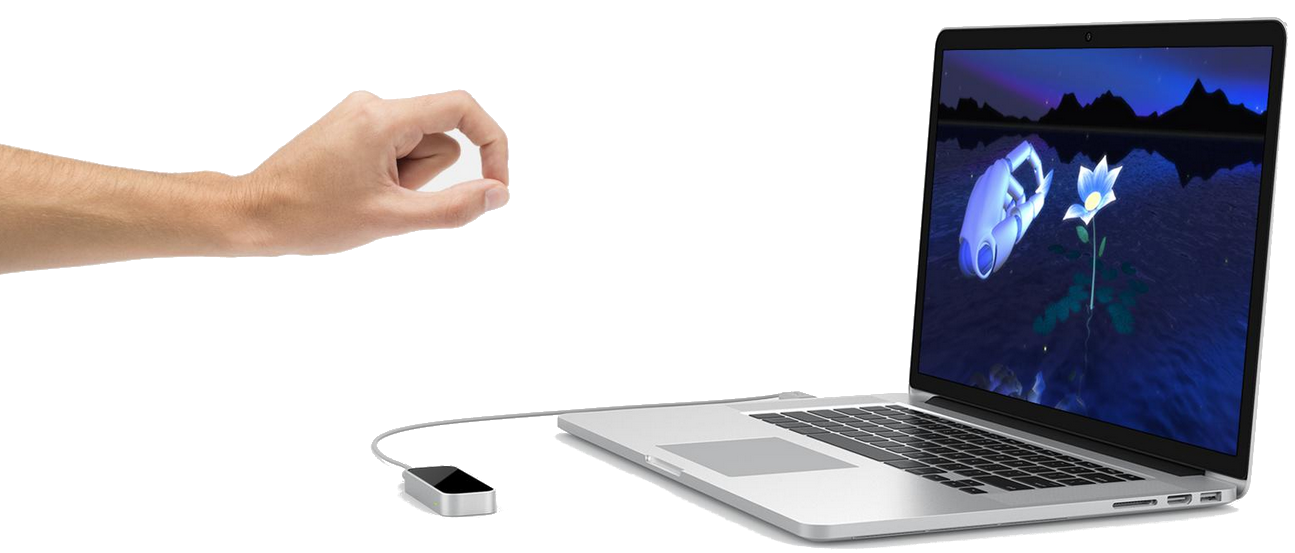
\includegraphics[scale=.3]{./Figures/LeapMotion.png}
\end{center}
\caption{Ejemplo del reconocimiento del gesto usando Leap Motion, mostrando mediante una aplicación donde los gestos son representados en 3D, que es el dispositivo que se encuentra conectado a la Laptop. Imagen recuperada de \ref{LeapMotionFN}.}
\label{fig:LeapMotion}
\end{figure}

El proceso de captura de los datos, la segmentación, la extracción de características, el seguimiento y el reconocimiento del dispositivo no se conoce a detalle, pues no ha sido publicado.\\ 
Solo se conoce \footnote{ \url{http://blog.leapmotion.com/hardware-to-software-how-does-the-leap-motion-controller-work/}} que se utilizan tres cámaras infrarrojas, con la imágenes obtenidas con se hace una representación 3D de las manos, antes de realizar el modelo las imágenes son segmentadas del fondo para eliminar el ruido generado por la iluminación u otros objetos que causen ruido en la imágenes. \\
Para realizar el seguimiento se extraen la características. Una de ellas son el dedos, el algoritmo de seguimiento interpreta la información 3D e infiere la posición de los objetos ocluidos. Se aplican filtros para suavizar los datos. 


Enseguida se explica el software de reconocimiento de gestos estáticos Flutter, fig:\ref{fig:Flutter} el cual reconoce cuatro gestos estáticos usando la cámara web como dispositivo de entrada. 

Se desconoce como funciona el software, solo se sabe que la mano es detectada por la cámara, para que la detección sea correcta la mano tiene que estar totalmente frente a la cámara web. Los algoritmos utilizados para el reconocimiento no se conocen.  
\begin{figure}[h!]
\begin{center}
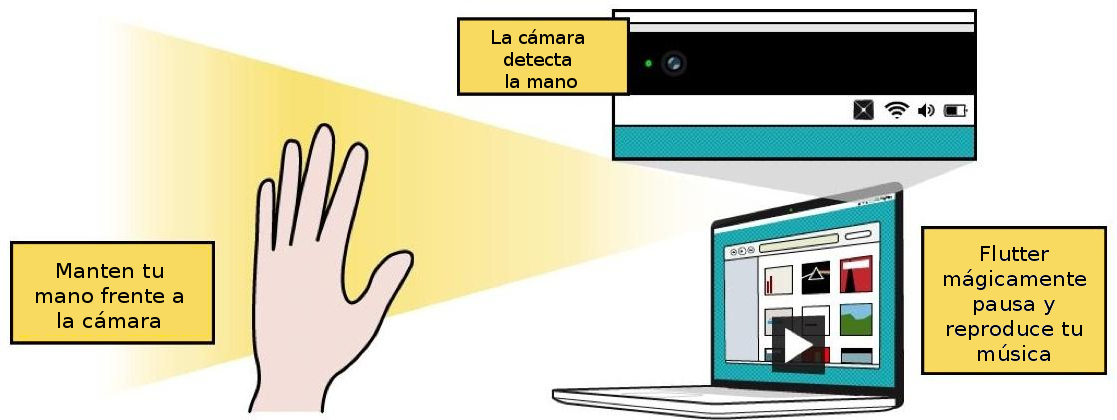
\includegraphics[scale=.4]{./Figures/Flutter.jpg}
\end{center}
\caption{La imagen anterior representa el funcionamiento del software Flutter. Imagen recuperada de \ref{FlutterFN} .}
\label{fig:Flutter}
\end{figure}

Flutter permite controlar aplicaciones multimedia como: YouTube \footnote{\url{https://www.youtube.com/}} ,VLC \footnote{\url{http://www.videolan.org/vlc/}}, Spotify \footnote{\url{https://www.spotify.com/}}, Netflix \footnote{\url{https://www.netflix.com/}}. Las limitaciones del software son que solo reconoce gestos estáticos. Una desventaja es que presenta falsos positivos al reconocer acciones del usuario.  

%::::::::::::::::::::::::::::::::::::::::::::::::::::::::::::::::::::::::::::::::::::::::::::::::::::::::: 

Aunque estos dispositivos y software para reconocer gestos solucionan algunos problemas importantes en el área, sigue existiendo el problema de bloqueo e iluminación.
De allí la importancia que existan nuevos modelos que ataquen estos problemas que se presentan frecuentemente en el reconocimiento de los gestos.
  
\section{Organizaci\'on de la tesis}\label{OrganizacionTesis}

La tesis se encuentra distribuida de la siguiente manera: la segunda sección presenta los fundamentos teóricos como base para la comprensión del tema. La tercera sección presenta la metodología utiliza en el sistema propuesto. En la cuarta sección se encuentran los detalles de la implementación del sistema. En la quinta sección están las pruebas realizadas al sistema junto con los resultados y las discusiones de estos. Finalmente la sexta sección presenta las conclusiones generales del sistema y el trabajo futuro. 


%EndExpansion
\newpage }

{\normalsize
%TCIMACRO{\QSubDoc{Include Capitulo02}{\chapter{Marco te\'orico}\label{capit:cap2}
\vspace{-2.0325ex}%
\noindent
\rule{\textwidth}{0.5pt}
\vspace{-5.5ex}% 
\newcommand{\pushline}{\Indp}% Indent puede ir o no :p

En este capítulo se definen una serie de conceptos importantes del área de procesamiento de imágenes y reconocimiento de patrones, estas definiciones son importantes para la comprensión del tema.


%--------------------------------------------------------------------------------------------------------------------------------


\section{Gestos}\label{sec:2Gestos}
Los gestos son movimientos del cuerpo expresivos y significativos que involucran dedos, manos, brazos, cabeza, cara o cuerpo con la intención de transmitir información relevante o interactuar con el ambiente \citep{Mitra2007}.
De acuerdo con la literatura los gestos con las manos se clasifican en estáticos y dinámicos, los primeros están definidos como la posición y orientación de la mano en el espacio manteniendo esta pose durante cierto tiempo, por ejemplo para hacer una se\~nal de aventón, a diferencia de los gestos dinámicos donde hay movimiento de la pose, un ejemplo  es cuando mueves la mano en se\~nal de adiós \citep{Mitra2007}. 


%--------------------------------------------------------------------------------------------------------------------------------

\section{Reconocimiento de gestos con la manos}\label{sec:2ReconocimientoGestos}   

El reconocimiento de gestos con las manos consiste no solo en el seguimiento del movimiento de la o las manos realizados por un emisor, también en la interpretación de este movimiento por un receptor, \citep{Mitra2007}, \citep{Murthy2009}.\\
De aquí en adelante entiéndase el término gestos con las manos, como gestos.   

Los métodos basados en la visión (ver Capitulo \ref{capit:cap1}, Sección \ref{sec:ReconocimientoGestos}) realizan la representación del gesto con diferentes técnicas las cuales se separan en dos categorías \citep{Rautaray2012}: basados en apariencia y basados en  modelo 3D. Los basados en modelo 3D convierten los datos en entrada en una forma espacial y los basados en apariencia utilizan los datos 2D de la imagen de entrada.      

De acuerdo con la literatura, el proceso de reconocimiento de gestos basados en la visión se dividen en tres fases que son: detección, extracción de características o seguimiento, dependiendo si los gestos son dinámicos, por último el reconocimiento del gesto \citep{Rautaray2012}. Otros autores incluyen la etapa de adquisición de datos \citep{Hasan2012}. Las etapas se abordarán en la sección siguiente. 


\subsection{Etapas del reconocimiento}\label{subsec:EtapasReconocimiento}  
En la sección se abordaron las etapas del reconocimiento y se mencionan los principales algoritmos utilizados en cada una de éstas. El diagrama de la Figura \ref{fig:HGR} muestra los diferentes pasos en el reconocimiento.  

\begin{figure}[h!]
\begin{center}

\includegraphics[scale=.6]{./Figures/HGR.png}
\end{center}
\caption{El diagrama ejemplifica el procedimiento del reconocimiento de gestos.}
\label{fig:HGR}
\end{figure}

El proceso de reconocimiento varía un poco dependiendo del tipo de gesto, si es estático o dinámico. Por ejemplo en la Figura \ref{fig:HGR} ejemplifica perfectamente el proceso de reconocimiento de un gesto estático, para los gestos dinámicos se necesita una fase extra, el seguimiento el cual se realiza una vez detectada la mano, puede estar englobada en la fase de extracción de características o viceversa. 


\subsubsection{Adquisición de datos}\label{sssec:EtapaAdquisicion}

Es la primera etapa del reconocimiento en la cual los datos son capturados. En el modelo basado en la visión se utilizan cámaras, el tipo de cámara depende del tipo de información que se quiera obtener de la mano. 

Las cámaras mas utilizadas son las RGB, con ellas se puede obtener información de la mano tales como la textura, forma, color, etc. Últimamente se han hecho muy populares las cámaras que proporcionan profundidad, tales como las basadas en tiempo de vuelo TOF, por sus siglas en inglés, o en luz estructurada. Estas cámaras generalmente se utilizan cuando se quiere obtener un modelo 3D de la mano, utilizando otra cámara normalmente RGB.



\subsubsection{Detección}\label{sssec:EtapaDeteccion}

En esta etapa se localiza y segmenta la mano del fondo de la imagen para obtener las características necesarias para identificar el gesto.
Existen distintos métodos para poder detectar la mano como: la de color de la piel, forma, movimiento, entre otras que generalmente son combinaciones de alguna de estas. Enseguida se describe brevemente cada una de estas.  
\begin{itemize}
\item Color de la piel: Se basa principalmente en escoger un espacio de color, es una organización de colores especifica; como; RGB (rojo, verde, azul), RG (rojo, green), YCrCb (brillo, la diferencia entre el brillo y el rojo, la diferencia entre el brillo y el azul), etc. La desventaja es que si es color de la piel es similar al fondo, la segmentación no es buena, la forma de corregir esta segmentación es suponiendo que el fondo no se mueve con respecto a la cámara.
\item Forma: Extrae el contorno de las imágenes, si se realiza correctamente se obtiene el contorno de la mano. Aunque si se toman las yemas de los dedos como características, éstas pueden ser obstruidas por el resto de la mano, una posible solución es usar más de una cámara.  
\item Valor de p\'ixeles: Usar imágenes en tonos de gris para detectar la mano con base en la apariencia y textura. Esto se logra entrenando un clasificador con un conjunto de imágenes.
\item Modelo 3D: Depende de cuál modelo se utilice, son las características de la mano requeridas. 
\item Movimiento: Generalmente ésta se usa con otras formas de detección ya que para utilizarse por sí sola hay que asumir que el único objeto con movimiento es la mano.
\end{itemize} 

La segmentación es la partición o separación de la imagen en regiones representativas, es decir separar la mano del fondo de la imagen. Existen diversos métodos para llevar acabo la segmentación de la mano los cuales se clasifican en tres clases, basados en pixeles los cuales hacen la separación usando el valor del nivel de gris en la imagen: en el borde estos métodos utilizan los pixeles que representan las orillas del objeto y encuentran el correspondiente contorno; en regiones los cuales van agrupando vecindarios de la imagen de acuerdo a ciertas propiedades; por último la segmentación basada en un modelo la cual hacen uso de algún modelo definido. Estos requieren imágenes de entrenamiento para representar la probabilidad de las muestras registradas y finalmente hace inferencias en la imagen \citep{Ibraheem2013}.

\subsubsection{Extracción de características y seguimiento}\label{sssec:EtapaSeguimiento}  

La extracción de características consiste en obtener ciertas entradas medibles de la imagen de la mano, generalmente segmentada, las cuales son utilizadas para reconocer el gesto realizado, \citep{Premaratne2013}, \citep{Nayakwadi2014}.

Existen dos tipos de características geométricas y no geométricas. Un ejemplo de características geométricas son las yemas de los dedos, la dirección de los dedos, el contorno de la mano y entre otras características. Y un ejemplo de características no geométricas son el color, siluetas y texturas de la mano. \citep{Murthy2009}. 

Enseguida se mencionan algunas de los métodos para la obtención de características \citep{Premaratne2013}. 
\begin{itemize}
\item Descriptores de Fourier los cuales describen formas en la imagen, haciendo uso de la serie de Fourier. Por ejemplo la forma de la pose de la mano.
\item Descriptores de Contorno nos dan el contorno  o el límite del objeto con invariancia a traslación, escala  y reflexión.     
\item Características descritas por histogramas. Histogramas de gradientes orientados (HOG) es un descriptor de características. Se trata de contar la orientación de los gradientes en cierta porción de la imagen.  
\end{itemize}


El seguimiento consiste en localizar la mano en cada cuadro (imagen). Se lleva acabo usando los métodos de detección si estos son lo suficientemente rápidos para detectar la mano cuadro por cuadro. Se explica brevemente algunos  métodos para llevar a cabo el seguimiento. 
\begin{itemize}
	\item Basado en plantillas: Este se divide en dos categorías (Características basadas en su correlación y basadas en contorno), que son similares a los métodos de detección, aunque supone que las imágenes son adquiridas con la frecuencia suficiente para llevar acabo el seguimiento. Características basadas en su correlación, sigue las características a través de cada cuadro, se asume que las características aparecen en mismo vecindario. Basadas en contorno, se basa en contornos deformables, consiste en colocar el contorno cerca de la región de interés e ir deformando este hasta encontrar la mano. 
	\item Estimación óptima: Consiste en usar filtros Kalman, un conjunto de ecuaciones matemáticas que proporciona una forma  computacionalmente eficiente y recursiva de estimar el estado de un proceso, de una manera que minimiza la media de un error cuadrático, el filtro soporta estimaciones del pasado, presente y futuros estados, y puede hacerlo incluso cuando la naturaleza precisa del modelo del sistema es desconocida;  para hacer la detección de características en la trayectoria. 
	\item Filtrado de partículas: Un método de estimación del estado de un sistema que cambia a lo largo del tiempo, este se compone de un conjunto de partículas (muestras) con pesos asignados, las partículas son estados posibles del proceso. Es utilizado cuando no se distingue bien la mano en la imagen. Por medio de partículas localiza la mano, la desventaja es que se requieren demasiadas partículas y  el seguimiento se vuelve imposible. 
	\item Camshift: Busca el objetivo, en este caso la mano, encuentra el patrón de distribución más similar en una secuencia de imágenes, la distribución es basada en el color. 
\end{itemize}

\subsubsection{Reconocimiento}\label{sssec:EtapaReconocimiento}

El reconocimiento es la etapa final de este proceso, el cual consiste en identificar el gesto utilizando alguna técnica de clasificación.\\
El método de clasificación a utilizar se elige dependiendo del tipo de gesto a reconocer, por ejemplo para los gestos estáticos se realiza el empatamiento del gesto con una plantilla previamente calculada; en los gestos dinámicos generalmente  se usan algoritmos de aprendizaje de máquina. Aunque los más utilizados son los algoritmos de redes neuronales, máquina de soporte vectorial y modelo oculto de Markov.\\ 
A continuación se encuentran los principales métodos para llevar acabo el reconocimiento del gestos \citep{Rautaray2012}. 
\begin{itemize}
	\item K-medias: Es un método de agrupamiento el cual consiste en determinar los $k$ puntos llamados centros para minimizar el error de agrupamiento, que es la suma de las distancias de todo los puntos al centro de cada grupo. El algoritmo empieza localizando aleatoriamente $k$ grupos en el espacio espectral. Cada p\'ixel en la imagen de entrada es entonces asignadas al centro del grupo mas cercano  
	\item Desplazamiento de medias: Es un método iterativo que encuentra el máximo en una función de densidad dada una muestra estadística de los datos.
	\item Máquinas de soporte vectorial: Consiste en un mapeo no lineal de los datos de entrada a un espacio de dimensi\'on m\'as grande, donde los datos pueden ser separados de forma lineal.  
	\item Modelo oculto de Markov: Es definido como un conjunto de estados, un estado inicial, un conjunto de símbolos de salida y un conjunto de estados de transición. En el reconocimiento de gestos se puede caracterizar a los estados como un conjunto de las posiciones de la mano; las  transiciones de los estados como la probabilidad de transición de cierta posición de la mano a otra; el símbolo de salida como una postura especifica y la secuencia de los símbolos de salida como  el gesto de la mano.   
	\item Redes neuronales con retraso: Son una clase de redes neuronales artificiales que se enfocan en datos continuos, haciendo que el sistema sea adaptable para redes en linea y les da ventajas sobre aplicaciones en tiempo real. 
\end{itemize}  


%--------------------------------------------------------------------------------------------------------------------------------


\section{Imagen}\label{ImagenDef} 

Una imagen se puede definir como una función bidimensional, $S(x,y)$ donde $x$, $y$ representan las coordenadas en el plano y el valor de la función es la intensidad o nivel de gris en el punto $(x,y)$. 
Si el valor de la función y los puntos de la imagen son finitos, esta es una imagen digital, la cual se puede representar en una matriz donde cada valor o pixel es el nivel de gris de la imagen, véase Figura \ref{fig:image}, y los indices de esta indican la posición, \citep{Gonzalez2002}. 

\begin{figure}[h!]
\begin{center}
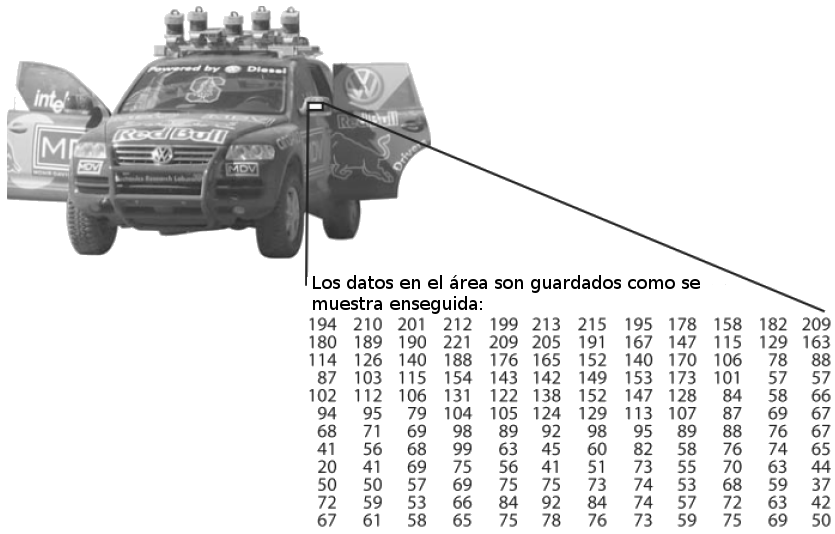
\includegraphics[scale=.50]{./Figures/image.png}
\end{center}
\caption{Representación de un imagen digital. Recuperada de \protect\citep{Shin2013}. }
\label{fig:image}
\end{figure}


%--------------------------------------------------------------------------------------------------------------------------------


\section{Obstrucción}\label{OclusionDef} 

Se puede definir una obstrucción como discontinuidades del movimiento y profundidad que se es percibida por un observador que se encuentra en movimiento en un ambiente estático.
Los puntos de obstrucción en una imagen o cuadro son pixeles que aparecen o desaparecen en dos cuadros consecutivos, estos son llamados puntos de obstrucción o punto de no obstrucción, \citep{Silva2001}.  

Existen tres tipos distintos de obstrucción las cuales dependen de la forma en que es causada. Estas son: obstrucción por el mismo objeto, entre objetos y por el fondo. La obstrucción por el mismo objeto se presenta cuando parte del objeto obstruye a otra. La obstrucción entre objetos es cuando dos objetos que se siguen se obstruyen entre ellos mismos. La obstrucción por el fondo es cuando parte del fondo obstruye al objeto que se sigue, \citep{YilmazA.JavedO.andShah2006}


%-------------------------------------------------------------------------------------------------------------------------------- 


\section{Métricas de desempeño}\label{Metricas}

Existen diversos métodos para medir el rendimiento de un algoritmo de clasificación, una manera de representarlo es mediante una matriz de confusión. 

Si consideramos una clasificación de un conjunto, donde cada elemento del conjunto es mapeado a un elemento del conjunto de etiquetas (positiva o negativa). El clasificador se encarga de mapear los elementos a las clases existentes, indicando la clase a la que pertenece la elemento.
El resultado de clasificación de algún elemento puede resultar en cuatro posibles estados. Si el elemento es positivo y la clasificación es positiva, es un verdadero positivo; si la clasificación es negativa es un falso negativo. Si el elemento es negativo y la clasificación es negativa, es un verdadero negativo; si la clasificación es positiva, es un falso positivo.  
Dado un clasificador y un conjunto de elementos, una matriz de confusión de $2 \times 2$, como la que se muestra en la Figura \ref{fig:Matrix}, puede ser construida por el resultado del conjunto de los elementos \citep{Fawcett2006}.   
\begin{figure}[h!]
\begin{center}
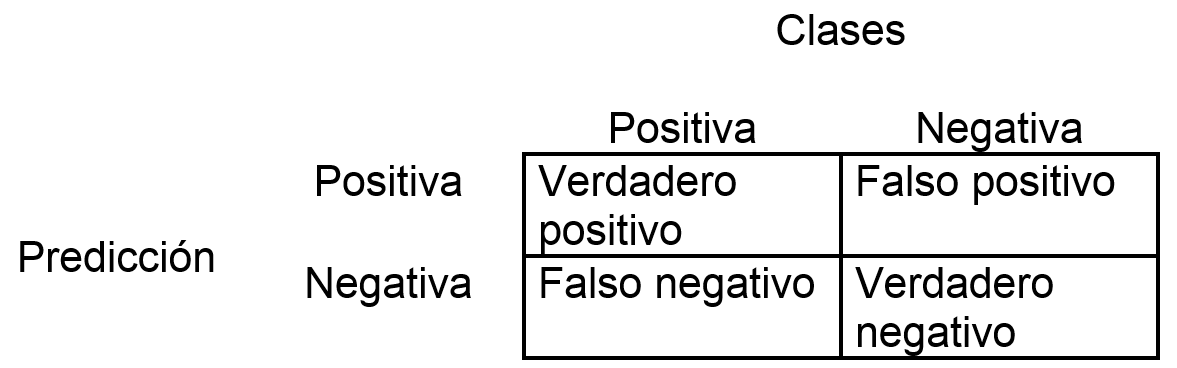
\includegraphics[scale=.4]{./Figures/MatrixConfusion.png}
\end{center}
\caption{La siguiente imagen representa una matriz de confusión, de un problema de clasificación de dos clases.}
\label{fig:Matrix}
\end{figure}
Los valores de la diaginal de la matriz de confusion representan las predicciones correctas, y los valores fuera de la diagonal representan los errores.

Distintas métricas de desempeño pueden ser calculadas gracias a esta matriz.\\ 
La tasa de precisi\'on del clasificador puede ser calculado como: 
\begin{equation}
Presici\'on = \frac{Verdaderos \quad positivos}{Verdaderos \quad positivos + Falsos \quad positivos}
\end{equation}
La tasa de exactitud del clasificador puede ser calculado como: 
\begin{equation}
Exactitud = \frac{Verdaderos \quad positivos + Verdaderos \quad negativos}{Total \quad de \quad positivos + Total \quad de \quad negativos}
\end{equation}
La tasa de verdaderos positivos $Tp$, del clasificador puede ser calculada como: 
\begin{equation}
Tp \approx \frac{Positivos \quad clasificados \quad correctamente}{Total \quad de \quad  positivos}
\end{equation} 
La tasa de falsos positivos $Fp$, del clasificador puede ser calculada como: 
\begin{equation}
Fp \approx \frac{Negativos \quad clasificados \quad correctamente}{Total \quad de \quad negativos}
\end{equation}






\newpage
%%=====================================================
} }%
%BeginExpansion
\chapter{Marco te\'orico}\label{capit:cap2}
\vspace{-2.0325ex}%
\noindent
\rule{\textwidth}{0.5pt}
\vspace{-5.5ex}% 
\newcommand{\pushline}{\Indp}% Indent puede ir o no :p

En este capítulo se definen una serie de conceptos importantes del área de procesamiento de imágenes y reconocimiento de patrones, estas definiciones son importantes para la comprensión del tema.


%--------------------------------------------------------------------------------------------------------------------------------


\section{Gestos}\label{sec:2Gestos}
Los gestos son movimientos del cuerpo expresivos y significativos que involucran dedos, manos, brazos, cabeza, cara o cuerpo con la intención de transmitir información relevante o interactuar con el ambiente \citep{Mitra2007}.
De acuerdo con la literatura los gestos con las manos se clasifican en estáticos y dinámicos, los primeros están definidos como la posición y orientación de la mano en el espacio manteniendo esta pose durante cierto tiempo, por ejemplo para hacer una se\~nal de aventón, a diferencia de los gestos dinámicos donde hay movimiento de la pose, un ejemplo  es cuando mueves la mano en se\~nal de adiós \citep{Mitra2007}. 


%--------------------------------------------------------------------------------------------------------------------------------

\section{Reconocimiento de gestos con la manos}\label{sec:2ReconocimientoGestos}   

El reconocimiento de gestos con las manos consiste no solo en el seguimiento del movimiento de la o las manos realizados por un emisor, también en la interpretación de este movimiento por un receptor, \citep{Mitra2007}, \citep{Murthy2009}.\\
De aquí en adelante entiéndase el término gestos con las manos, como gestos.   

Los métodos basados en la visión (ver Capitulo \ref{capit:cap1}, Sección \ref{sec:ReconocimientoGestos}) realizan la representación del gesto con diferentes técnicas las cuales se separan en dos categorías \citep{Rautaray2012}: basados en apariencia y basados en  modelo 3D. Los basados en modelo 3D convierten los datos en entrada en una forma espacial y los basados en apariencia utilizan los datos 2D de la imagen de entrada.      

De acuerdo con la literatura, el proceso de reconocimiento de gestos basados en la visión se dividen en tres fases que son: detección, extracción de características o seguimiento, dependiendo si los gestos son dinámicos, por último el reconocimiento del gesto \citep{Rautaray2012}. Otros autores incluyen la etapa de adquisición de datos \citep{Hasan2012}. Las etapas se abordarán en la sección siguiente. 


\subsection{Etapas del reconocimiento}\label{subsec:EtapasReconocimiento}  
En la sección se abordaron las etapas del reconocimiento y se mencionan los principales algoritmos utilizados en cada una de éstas. El diagrama de la Figura \ref{fig:HGR} muestra los diferentes pasos en el reconocimiento.  

\begin{figure}[h!]
\begin{center}

\includegraphics[scale=.6]{./Figures/HGR.png}
\end{center}
\caption{El diagrama ejemplifica el procedimiento del reconocimiento de gestos.}
\label{fig:HGR}
\end{figure}

El proceso de reconocimiento varía un poco dependiendo del tipo de gesto, si es estático o dinámico. Por ejemplo en la Figura \ref{fig:HGR} ejemplifica perfectamente el proceso de reconocimiento de un gesto estático, para los gestos dinámicos se necesita una fase extra, el seguimiento el cual se realiza una vez detectada la mano, puede estar englobada en la fase de extracción de características o viceversa. 


\subsubsection{Adquisición de datos}\label{sssec:EtapaAdquisicion}

Es la primera etapa del reconocimiento en la cual los datos son capturados. En el modelo basado en la visión se utilizan cámaras, el tipo de cámara depende del tipo de información que se quiera obtener de la mano. 

Las cámaras mas utilizadas son las RGB, con ellas se puede obtener información de la mano tales como la textura, forma, color, etc. Últimamente se han hecho muy populares las cámaras que proporcionan profundidad, tales como las basadas en tiempo de vuelo TOF, por sus siglas en inglés, o en luz estructurada. Estas cámaras generalmente se utilizan cuando se quiere obtener un modelo 3D de la mano, utilizando otra cámara normalmente RGB.



\subsubsection{Detección}\label{sssec:EtapaDeteccion}

En esta etapa se localiza y segmenta la mano del fondo de la imagen para obtener las características necesarias para identificar el gesto.
Existen distintos métodos para poder detectar la mano como: la de color de la piel, forma, movimiento, entre otras que generalmente son combinaciones de alguna de estas. Enseguida se describe brevemente cada una de estas.  
\begin{itemize}
\item Color de la piel: Se basa principalmente en escoger un espacio de color, es una organización de colores especifica; como; RGB (rojo, verde, azul), RG (rojo, green), YCrCb (brillo, la diferencia entre el brillo y el rojo, la diferencia entre el brillo y el azul), etc. La desventaja es que si es color de la piel es similar al fondo, la segmentación no es buena, la forma de corregir esta segmentación es suponiendo que el fondo no se mueve con respecto a la cámara.
\item Forma: Extrae el contorno de las imágenes, si se realiza correctamente se obtiene el contorno de la mano. Aunque si se toman las yemas de los dedos como características, éstas pueden ser obstruidas por el resto de la mano, una posible solución es usar más de una cámara.  
\item Valor de p\'ixeles: Usar imágenes en tonos de gris para detectar la mano con base en la apariencia y textura. Esto se logra entrenando un clasificador con un conjunto de imágenes.
\item Modelo 3D: Depende de cuál modelo se utilice, son las características de la mano requeridas. 
\item Movimiento: Generalmente ésta se usa con otras formas de detección ya que para utilizarse por sí sola hay que asumir que el único objeto con movimiento es la mano.
\end{itemize} 

La segmentación es la partición o separación de la imagen en regiones representativas, es decir separar la mano del fondo de la imagen. Existen diversos métodos para llevar acabo la segmentación de la mano los cuales se clasifican en tres clases, basados en pixeles los cuales hacen la separación usando el valor del nivel de gris en la imagen: en el borde estos métodos utilizan los pixeles que representan las orillas del objeto y encuentran el correspondiente contorno; en regiones los cuales van agrupando vecindarios de la imagen de acuerdo a ciertas propiedades; por último la segmentación basada en un modelo la cual hacen uso de algún modelo definido. Estos requieren imágenes de entrenamiento para representar la probabilidad de las muestras registradas y finalmente hace inferencias en la imagen \citep{Ibraheem2013}.

\subsubsection{Extracción de características y seguimiento}\label{sssec:EtapaSeguimiento}  

La extracción de características consiste en obtener ciertas entradas medibles de la imagen de la mano, generalmente segmentada, las cuales son utilizadas para reconocer el gesto realizado, \citep{Premaratne2013}, \citep{Nayakwadi2014}.

Existen dos tipos de características geométricas y no geométricas. Un ejemplo de características geométricas son las yemas de los dedos, la dirección de los dedos, el contorno de la mano y entre otras características. Y un ejemplo de características no geométricas son el color, siluetas y texturas de la mano. \citep{Murthy2009}. 

Enseguida se mencionan algunas de los métodos para la obtención de características \citep{Premaratne2013}. 
\begin{itemize}
\item Descriptores de Fourier los cuales describen formas en la imagen, haciendo uso de la serie de Fourier. Por ejemplo la forma de la pose de la mano.
\item Descriptores de Contorno nos dan el contorno  o el límite del objeto con invariancia a traslación, escala  y reflexión.     
\item Características descritas por histogramas. Histogramas de gradientes orientados (HOG) es un descriptor de características. Se trata de contar la orientación de los gradientes en cierta porción de la imagen.  
\end{itemize}


El seguimiento consiste en localizar la mano en cada cuadro (imagen). Se lleva acabo usando los métodos de detección si estos son lo suficientemente rápidos para detectar la mano cuadro por cuadro. Se explica brevemente algunos  métodos para llevar a cabo el seguimiento. 
\begin{itemize}
	\item Basado en plantillas: Este se divide en dos categorías (Características basadas en su correlación y basadas en contorno), que son similares a los métodos de detección, aunque supone que las imágenes son adquiridas con la frecuencia suficiente para llevar acabo el seguimiento. Características basadas en su correlación, sigue las características a través de cada cuadro, se asume que las características aparecen en mismo vecindario. Basadas en contorno, se basa en contornos deformables, consiste en colocar el contorno cerca de la región de interés e ir deformando este hasta encontrar la mano. 
	\item Estimación óptima: Consiste en usar filtros Kalman, un conjunto de ecuaciones matemáticas que proporciona una forma  computacionalmente eficiente y recursiva de estimar el estado de un proceso, de una manera que minimiza la media de un error cuadrático, el filtro soporta estimaciones del pasado, presente y futuros estados, y puede hacerlo incluso cuando la naturaleza precisa del modelo del sistema es desconocida;  para hacer la detección de características en la trayectoria. 
	\item Filtrado de partículas: Un método de estimación del estado de un sistema que cambia a lo largo del tiempo, este se compone de un conjunto de partículas (muestras) con pesos asignados, las partículas son estados posibles del proceso. Es utilizado cuando no se distingue bien la mano en la imagen. Por medio de partículas localiza la mano, la desventaja es que se requieren demasiadas partículas y  el seguimiento se vuelve imposible. 
	\item Camshift: Busca el objetivo, en este caso la mano, encuentra el patrón de distribución más similar en una secuencia de imágenes, la distribución es basada en el color. 
\end{itemize}

\subsubsection{Reconocimiento}\label{sssec:EtapaReconocimiento}

El reconocimiento es la etapa final de este proceso, el cual consiste en identificar el gesto utilizando alguna técnica de clasificación.\\
El método de clasificación a utilizar se elige dependiendo del tipo de gesto a reconocer, por ejemplo para los gestos estáticos se realiza el empatamiento del gesto con una plantilla previamente calculada; en los gestos dinámicos generalmente  se usan algoritmos de aprendizaje de máquina. Aunque los más utilizados son los algoritmos de redes neuronales, máquina de soporte vectorial y modelo oculto de Markov.\\ 
A continuación se encuentran los principales métodos para llevar acabo el reconocimiento del gestos \citep{Rautaray2012}. 
\begin{itemize}
	\item K-medias: Es un método de agrupamiento el cual consiste en determinar los $k$ puntos llamados centros para minimizar el error de agrupamiento, que es la suma de las distancias de todo los puntos al centro de cada grupo. El algoritmo empieza localizando aleatoriamente $k$ grupos en el espacio espectral. Cada p\'ixel en la imagen de entrada es entonces asignadas al centro del grupo mas cercano  
	\item Desplazamiento de medias: Es un método iterativo que encuentra el máximo en una función de densidad dada una muestra estadística de los datos.
	\item Máquinas de soporte vectorial: Consiste en un mapeo no lineal de los datos de entrada a un espacio de dimensi\'on m\'as grande, donde los datos pueden ser separados de forma lineal.  
	\item Modelo oculto de Markov: Es definido como un conjunto de estados, un estado inicial, un conjunto de símbolos de salida y un conjunto de estados de transición. En el reconocimiento de gestos se puede caracterizar a los estados como un conjunto de las posiciones de la mano; las  transiciones de los estados como la probabilidad de transición de cierta posición de la mano a otra; el símbolo de salida como una postura especifica y la secuencia de los símbolos de salida como  el gesto de la mano.   
	\item Redes neuronales con retraso: Son una clase de redes neuronales artificiales que se enfocan en datos continuos, haciendo que el sistema sea adaptable para redes en linea y les da ventajas sobre aplicaciones en tiempo real. 
\end{itemize}  


%--------------------------------------------------------------------------------------------------------------------------------


\section{Imagen}\label{ImagenDef} 

Una imagen se puede definir como una función bidimensional, $S(x,y)$ donde $x$, $y$ representan las coordenadas en el plano y el valor de la función es la intensidad o nivel de gris en el punto $(x,y)$. 
Si el valor de la función y los puntos de la imagen son finitos, esta es una imagen digital, la cual se puede representar en una matriz donde cada valor o pixel es el nivel de gris de la imagen, véase Figura \ref{fig:image}, y los indices de esta indican la posición, \citep{Gonzalez2002}. 

\begin{figure}[h!]
\begin{center}
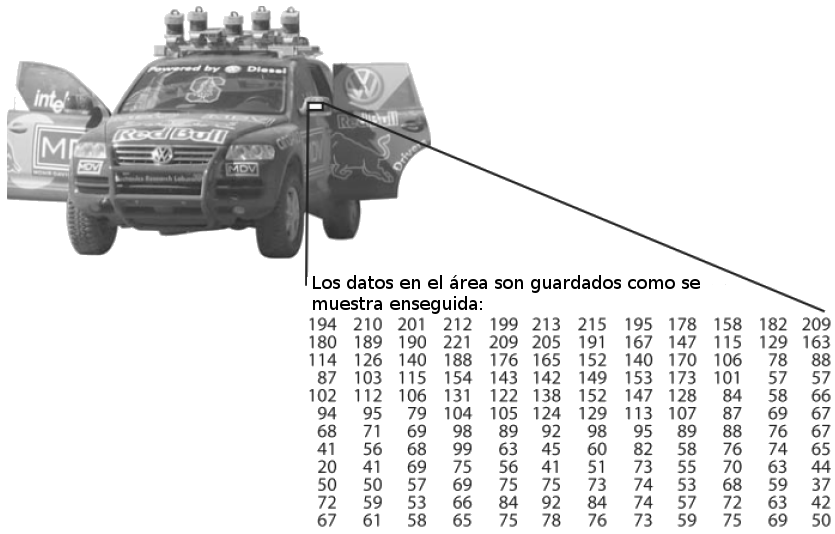
\includegraphics[scale=.50]{./Figures/image.png}
\end{center}
\caption{Representación de un imagen digital. Recuperada de \protect\citep{Shin2013}. }
\label{fig:image}
\end{figure}


%--------------------------------------------------------------------------------------------------------------------------------


\section{Obstrucción}\label{OclusionDef} 

Se puede definir una obstrucción como discontinuidades del movimiento y profundidad que se es percibida por un observador que se encuentra en movimiento en un ambiente estático.
Los puntos de obstrucción en una imagen o cuadro son pixeles que aparecen o desaparecen en dos cuadros consecutivos, estos son llamados puntos de obstrucción o punto de no obstrucción, \citep{Silva2001}.  

Existen tres tipos distintos de obstrucción las cuales dependen de la forma en que es causada. Estas son: obstrucción por el mismo objeto, entre objetos y por el fondo. La obstrucción por el mismo objeto se presenta cuando parte del objeto obstruye a otra. La obstrucción entre objetos es cuando dos objetos que se siguen se obstruyen entre ellos mismos. La obstrucción por el fondo es cuando parte del fondo obstruye al objeto que se sigue, \citep{YilmazA.JavedO.andShah2006}


%-------------------------------------------------------------------------------------------------------------------------------- 


\section{Métricas de desempeño}\label{Metricas}

Existen diversos métodos para medir el rendimiento de un algoritmo de clasificación, una manera de representarlo es mediante una matriz de confusión. 

Si consideramos una clasificación de un conjunto, donde cada elemento del conjunto es mapeado a un elemento del conjunto de etiquetas (positiva o negativa). El clasificador se encarga de mapear los elementos a las clases existentes, indicando la clase a la que pertenece la elemento.
El resultado de clasificación de algún elemento puede resultar en cuatro posibles estados. Si el elemento es positivo y la clasificación es positiva, es un verdadero positivo; si la clasificación es negativa es un falso negativo. Si el elemento es negativo y la clasificación es negativa, es un verdadero negativo; si la clasificación es positiva, es un falso positivo.  
Dado un clasificador y un conjunto de elementos, una matriz de confusión de $2 \times 2$, como la que se muestra en la Figura \ref{fig:Matrix}, puede ser construida por el resultado del conjunto de los elementos \citep{Fawcett2006}.   
\begin{figure}[h!]
\begin{center}
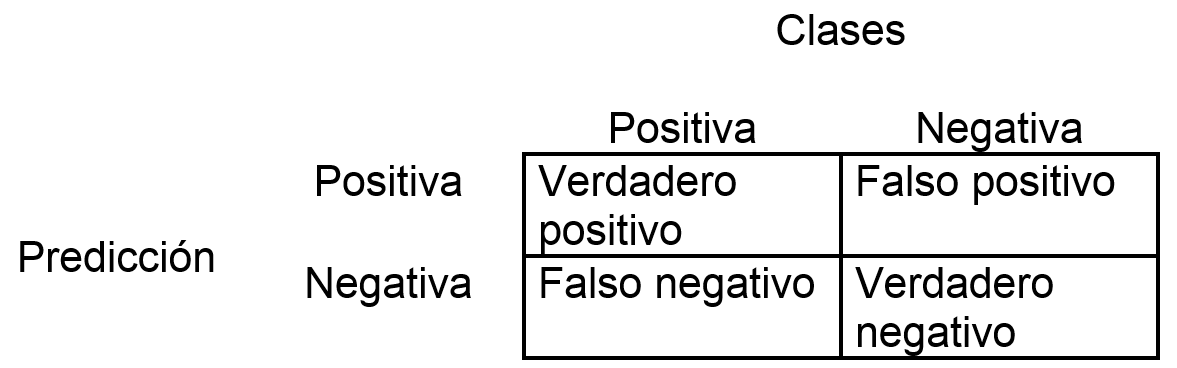
\includegraphics[scale=.4]{./Figures/MatrixConfusion.png}
\end{center}
\caption{La siguiente imagen representa una matriz de confusión, de un problema de clasificación de dos clases.}
\label{fig:Matrix}
\end{figure}
Los valores de la diaginal de la matriz de confusion representan las predicciones correctas, y los valores fuera de la diagonal representan los errores.

Distintas métricas de desempeño pueden ser calculadas gracias a esta matriz.\\ 
La tasa de precisi\'on del clasificador puede ser calculado como: 
\begin{equation}
Presici\'on = \frac{Verdaderos \quad positivos}{Verdaderos \quad positivos + Falsos \quad positivos}
\end{equation}
La tasa de exactitud del clasificador puede ser calculado como: 
\begin{equation}
Exactitud = \frac{Verdaderos \quad positivos + Verdaderos \quad negativos}{Total \quad de \quad positivos + Total \quad de \quad negativos}
\end{equation}
La tasa de verdaderos positivos $Tp$, del clasificador puede ser calculada como: 
\begin{equation}
Tp \approx \frac{Positivos \quad clasificados \quad correctamente}{Total \quad de \quad  positivos}
\end{equation} 
La tasa de falsos positivos $Fp$, del clasificador puede ser calculada como: 
\begin{equation}
Fp \approx \frac{Negativos \quad clasificados \quad correctamente}{Total \quad de \quad negativos}
\end{equation}






\newpage
%%=====================================================

%EndExpansion
\newpage }

{\normalsize
%TCIMACRO{\QSubDoc{Include Capitulo03}{\chapter{Sistema propuesto de reconocimiento de gestos}\label{capit:cap3}
\vspace{-2.0325ex}%
\noindent
\rule{\textwidth}{0.5pt}
\vspace{-5.5ex}% 
\newcommand{\pushline}{\Indp}% Indent puede ir o no :p 

En este cap\'itulo se describen las etapas del sistema propuesto junto con los métodos y algoritmos que son utilizados en cada una de las fases.
 
El sistema propuesto de reconocimiento de gestos consta de cuatro etapas principales, Figura \ref{fig:MyHGR}. La primera etapa es la adquisición de los datos, en la cual se capturan las imágenes de entrada del sistema. La siguiente etapa es la detección, aquí la mano es localizada y segmentada del fondo. En la etapa tres se extraen las características de la mano para ser procesadas. En la etapa final el gesto realizado es reconocido.   

\begin{figure}[h!]
\begin{center}

\includegraphics[scale=.6]{./Figures/MyHGR.png}
\end{center}
\caption{Metodología del sistema propuesto.}
\label{fig:MyHGR}
\end{figure}  
  
\section{Adquisición de los datos}\label{sec:KinectSensor} 

En la primera etapa del sistema los datos de entrada del sistema son capturados y preprocesados, la Figura \ref{fig:Dadquisicion} muestra las etapas de este proceso. Los datos provienen de los sensores de profundidad de dos dispositivos Kinect. Debido a la naturaleza del sensor las imágenes capturadas contiene ruido por interferencia \citep{Mallick2014}, que puede ser reducido utilizando filtro de medianas \citep{Maimone2011}.

\begin{figure}[h!]
\begin{center}
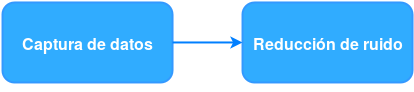
\includegraphics[scale=.6]{./Figures/Adquisicion.png}
\end{center}
\caption{Proceso de la etapa de adquisición de datos.} 
\label{fig:Dadquisicion}
\end{figure}   


\subsection{Kinect}

En noviembre del 2010 la compa\'nia Microsoft lanz\'o el sensor Kinect para consolas de vídeo juego Xbox 360 y en febrero del 2011 lanz\'o la versi\'on para Windows. El dispositivo fue desarrollado por la compa\~nia PrimeSense en conjunto con Microsoft \footnote{\url{engadget.com/2013/06/21/life-after-kinect-primesense-post-microsoft/}}. El sensor de profundidad que utiliza el dispositivo fue desarrollado por Zeev Zalesvky, Alexanser Shpunt, Aviad Maizels y Javier Garcia en 2005 \footnote{\url{https://patentscope.wipo.int/search/en/detail.jsf?docId=WO2007043036&recNum=1&maxRec=&office=&prevFilter=&sortOption=&queryString=&tab=PCT+Biblio}}   


El dispositivo Kinect está equipado con una serie de sensores que permiten obtener imágenes a color y de profundidad (las cuales indican la distancia a la que está ubicada un objeto del sensor). La Figura \ref{fig:KinectPic} muestra la parte frontal del dispositivo Kinect para Windows. Los sensores permiten hacer detección y seguimiento de personas. El dispositivo tiene la capacidad de detectar hasta seis personas y hacer el seguimiento de hasta dos personas \footnote{\url{https://msdn.microsoft.com/en-us/library/hh973074.aspx}}.    
  
\begin{figure}[h!]
\begin{center}
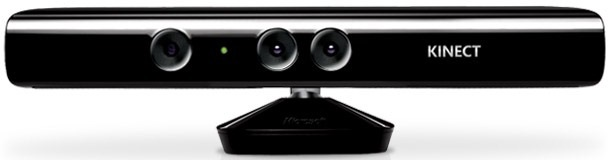
\includegraphics[scale=.65]{./Figures/Kinect.jpg}
\end{center}
\caption{Parte frontal del dispositivo Kinect en su versión para Windows, imagen recuperada de \protect\footnotemark{}.} 
\label{fig:KinectPic}
\end{figure} 

\footnotetext{\url{http://goo.gl/2GlwI}}

El sensor está equipado con los siguientes componentes: un cámara de color (o sensor de color), un emisor infrarrojo, un sensor infrarrojo de profundidad, un motor que controla la inclinación, un arreglo de cuatro micrófonos y un LED \citep{Jana2013}.
Enseguida se describen brevemente cada uno de los componentes del sensor Kinect, estos se muestran en la Figura \ref{fig:KinectComponentes}. 

\begin{figure}[h!]
\begin{center}
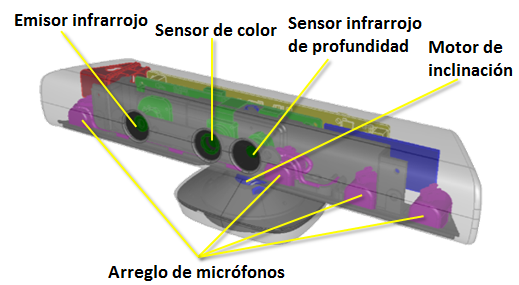
\includegraphics[scale=.6]{./Figures/sensor.png}
\end{center}
\caption{Componentes del sensor Kinect, imagen recuperada de \footnotemark{}.} 
\label{fig:KinectComponentes}
\end{figure}   

\footnotetext{\url{https://msdn.microsoft.com/en-us/library/jj131033.aspx}}

\begin{itemize}
\item La cámara de color captura y transmite datos de vídeo a color, detectando los colores rojo, verde y azul (RGB, por sus siglas en ingl\'es, red, green and blue). La transmisión de datos que brinda la cámara es una secuencia de imágenes (cuadros), a una velocidad de hasta treinta cuadros por segundo con una resolución de hasta $1280\, x \, 960$ p\'ixeles. La velocidad de los cuadros por segundo varia según la resolución de la imagen.

\item El emisor infrarrojo proyecta puntos de luz infrarroja, estos puntos son proyectados frente al sensor. Estos puntos junto con el sensor de profundidad es posible medir la distancia que existe del sensor a algún objeto que esté frente a él.  

\item El sensor infrarrojo lee los puntos infrarrojos proyectados por el emisor infrarrojo, con la lectura de los datos se calcula la distancia que existe entre el objeto y el sensor. El sensor transmite los datos de profundidad con una velocidad de hasta treinta cuadros por segundo con una resolución de hasta $640 \, x \, 480$ pixeles.   

\item El motor de inclinación controla el \'angulo de la posición vertical de los sensores del dispositivo. El motor puede moverse desde un \'angulo de $-27^ \circ$ a $+27^\circ$, con respecto al eje vertical del sensor.  

\item La entrada de audio compuesta por un arreglo de cuatro micrófonos permite capturar el sonido y calcular la posición de la fuente.

\item LED indica el estado del sensor. El LED en color verde indica que el sensor está disponible para utilizarse. El LED en color rojo indica que no existe conexión entre el Kinect y la computadora. La ausencia de color en el LED indica que el Kinect no se encuentra conectado a la fuente de energía eléctrica.
\end{itemize}

\subsection{Filtro de mediana} 

Existen distintos métodos para eliminar el ruido por interferencia causado por dos o más  Kinect, algunos de estos métodos son invasivos pues el hardware del Kinect es modificado \citep{Mallick2014}. Una opción es utilizar filtro de mediana, debido a que rellena los valores faltantes en la imagen proveniente del Kinect \citep{Maimone2011}. 

Sea $W_{mn}$ el vecindario de tamaño $m \times n$, centrado en el pixel, $s$, que se encuentra en la posición $(x,y)$. El filtro de mediana de la imagen $S(x,y)$, se calcula como: 
\begin{equation}
s(x,y)=\underset{(u,v)\in W_{mn}}{\text{mediana}} \lbrace S(u,v)\rbrace
\end{equation}

El filtro de mediana reemplaza el valor del pixel usando la mediana de las intensidades del vecindario del pixel, el valor del pixel en la posición (x,y) es incluido en el calculo \citep{Gonzalez2002}. 
 

%:::::::::::::::::::::::::::::::::::::::::::::::::::::::::::::::::::::::::::::::::::::::::::::::::::::::::::::::::::::::::::::::::::::::


\section{Detección}\label{sec:Detection}

En esta etapa del sistema el objetivo es localizar la mano en la imagen y segmentar la mano del fondo de la imagen. Para extraer las características necesarias para el reconocimiento.
La Figura \ref{fig:ProcesoDeteccion} muestra el proceso para  realizar la etapa de detección. El primer paso es localizar la mano, en este trabajo se utiliza el método de detección rápida de objetos; el siguiente paso es segmentar la mano del fondo, binarizando la imagen de la mano usando el algoritmo propuesto por \citep{Otsu1979}; finalmente se aplican las operaciones morfológicas apertura y cierre, para mejorar la segmentación, es decir eliminar ruido existente. 

\begin{figure}[h!]
\begin{center}
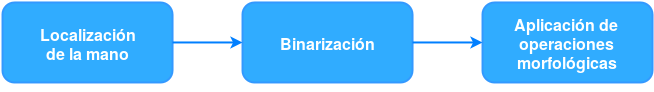
\includegraphics[scale=.7]{./Figures/Detection.png}
\end{center}
\caption{Proceso de detección de la mano.}
\label{fig:ProcesoDeteccion}
\end{figure} 

\subsection{Método detección rápida de objetos usando características simples utilizando el clasificador AdaBoost en forma de cascada}\label{subsec:ViolaJones}

En este trabajo se utiliza el método detección rápida de objetos usando características simples utilizando el clasificador AdaBoost en forma de cascada propuesto por \citep{Viola2001}, el cual fue creado originalmente para atacar el problema de detección de rostros. El método puede ser usando para detectar cualquier objeto debido a que la detección se realiza clasificando imágenes basándose en el valor de características simples.

La técnica detecta si el objeto se encuentra en la escena, usando una versión modificada del clasificador AdaBoost \citep{Freund1995} en forma de cascada y discrimina el objeto tomando en cuenta el valor de las características Haar \citep{Viola2001}. Las características son seleccionadas usando también el clasificador AdaBoost y el valor de éstas es calculado mediante el uso de una imagen integral \citep{Viola2001}. 

La Figura \ref{fig:ViolaJonesDiagram} muestra un diagrama del proceso del método de detección, el primer paso es obtener la muestras de entrenamiento con las cuales se construirá el clasificador; el siguiente paso es seleccionar las características que formarán el clasificador. Estas se escogen mediante el algoritmo de AdaBoost y su valor es calculado usando la imagen integral. El paso final  involucra construir el clasificador mediante el uso de Adaboost,  en forma de cascada.

\begin{figure}[h!]
\begin{center}
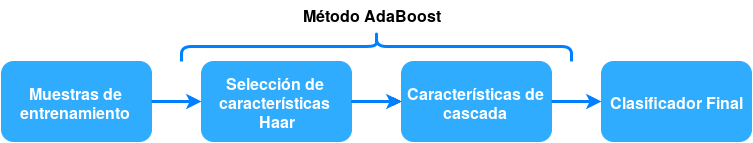
\includegraphics[scale=.6]{./Figures/ViolaJonesDiagram.png}
\end{center}
\caption{Procedimiento del algoritmo de detección rápida de objetos.}
\label{fig:ViolaJonesDiagram}
\end{figure}

Enseguida se explica a detalle cada etapa del método \citep{Viola2001}. 

\subsubsection{Características Haar}\label{sssec:CaracteristicasHaar}  

Las características Haar, son operadores rectangulares como los que se muestran en la Figura \ref{fig:haarFeatures}. A continuación se explicarán los operadores Haar básicos:
\begin{itemize}
\item Las características con dos rectángulos Figura \ref{fig:haarFeatures:1}, Figura \ref{fig:haarFeatures:2}, contienen dos regiones rectangulares adyacentes, el valor de la característica se calcula tomando la diferencia de la suma de ambas regiones. 

\item Las características con tres rectángulos Figura \ref{fig:haarFeatures:3}, contienen tres regiones rectangulares adyacentes, el valor de la característica se calcula sumando las regiones exteriores y restando la suma de la región interior.

\item Las características con cuatro rectángulos Figura \ref{fig:haarFeatures:4}, contienen cuatro regiones rectangulares adyacentes, el valor de la característica se obtiene con la diferencia entre la suma de las regiones pares diagonales.
\end{itemize} 

\begin{figure}[h!]
\centering
\subfigure[]{
\includegraphics[scale=.4]{./Figures/haarFeatures1}\label{fig:haarFeatures:1}}
\subfigure[]{
\includegraphics[scale=.4]{./Figures/haarFeatures2}\label{fig:haarFeatures:2}}
\subfigure[]{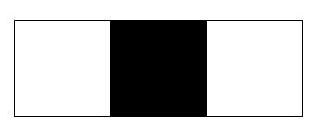
\includegraphics[scale=.4]{./Figures/haarFeatures3}\label{fig:haarFeatures:3}}
\subfigure[]{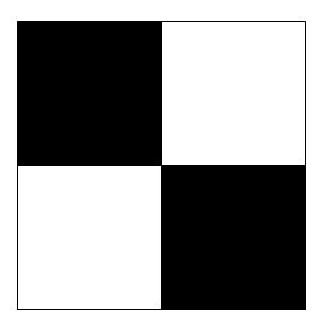
\includegraphics[scale=.4]{./Figures/haarFeatures4}\label{fig:haarFeatures:4}}
\caption{Ejemplo de tipos de operadores Haar.} \label{fig:haarFeatures}
\end{figure}


\subsubsection{Imagen integral}\label{sssec:IntegralImage} 

Uno de los aportes del método desarrollado por Viola y Jones es el concepto de imagen integral con la cual se calcula el valor de las características de manera rápida, es decir en tiempo constante, $O(1)$.  

La imagen integral, $SI$, de una imagen, $S(x,y)$, es calculada como la suma del valor de los pixeles que se encuentran arriba y a la izquierda de cierta posición de la imagen a la cual se le quiere hacer el cálculo. Lo anterior se puede escribir como: \footnote{\url{https://goo.gl/0oIJBz}}   
\begin{equation}
SI(x,y)=S(x,y) + S(x-1,y) + SI(x,y-1)-SI(x-1,y-1).
\end{equation}   
La Figura \ref{fig:FigIntegralImage} muestra un  ejemplo donde se calcula la imagen integral, Figura \ref{fig:FigIntegralImage:2}, de la imagen original Figura \ref{fig:FigIntegralImage:1}.
\begin{figure}[h!]
\centering
\subfigure[Imagen original]{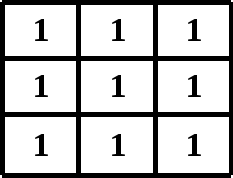
\includegraphics[scale=.6]{./Figures/ImagetoIntegral}\label{fig:FigIntegralImage:1}} \qquad
\subfigure[Imagen integral]{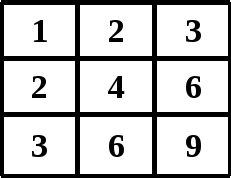
\includegraphics[scale=.6]{./Figures/CalculationIntegral}\label{fig:FigIntegralImage:2}}
\caption{Ejemplo del cálculo de la imagen integral.} 
\label{fig:FigIntegralImage}
\end{figure}

La imagen integral permite calcular la suma de los pixeles de cierta región usando solo los valores de las esquinas de la imagen integral de dicha región, la cual se obtiene como: \footnote{\url{https://goo.gl/0oIJBz}}    
\begin{equation}
REG(\alpha)=SI(A)+SI(D)-SI(B)-SI(C),
\end{equation}
donde $REG(\alpha)$ es la región a la cual se quiere calcular el valor de la suma de sus pixeles; $A,B,C,D$ son las esquinas de dicha región. Como se muestra en la Figura \ref{fig:figImageIntegral}, la región $\alpha$ se encuentra resaltada en color azul.  
\begin{figure}[h!]
\begin{center}
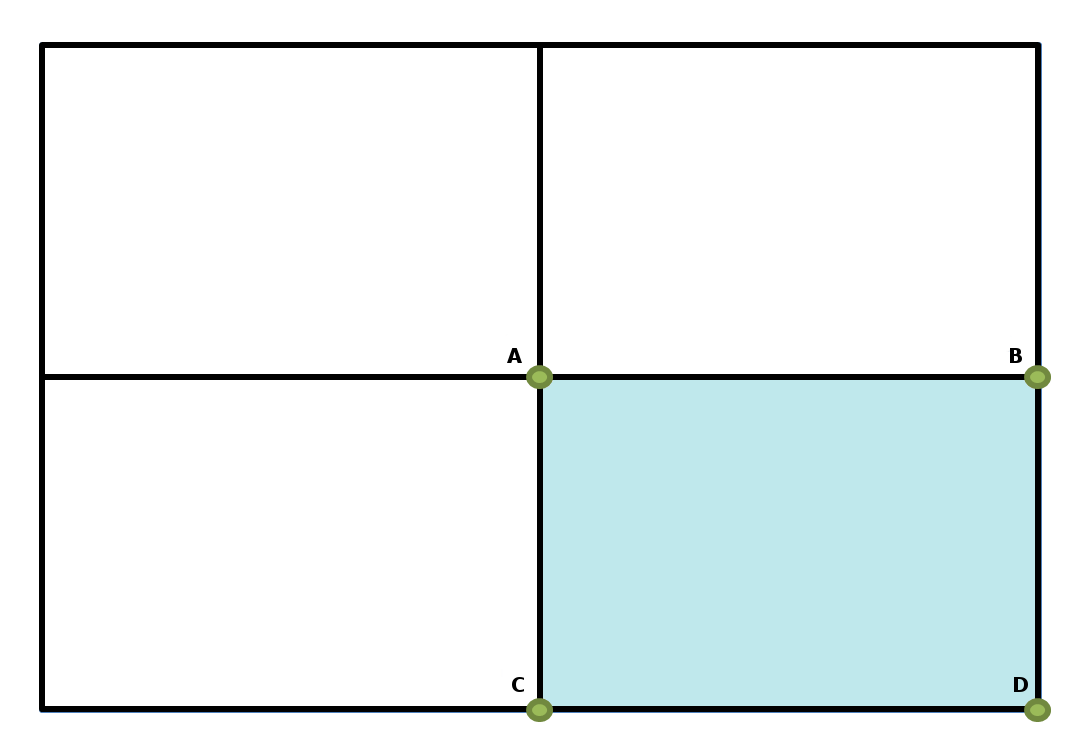
\includegraphics[scale=.25]{./Figures/IntegralImage.png}
\end{center}
\caption{Regiones de la imagen integral.}
\label{fig:figImageIntegral}
\end{figure} 


\subsubsection{Algoritmo AdaBoost}\label{sssec:AdaboostClasifier}  

En el método de detección el clasificador AdaBoost es utilizado para seleccionar las características relevantes, con las cuales se podrá detectar el objeto. También es utilizado para construir el clasificador final pero en forma de cascada, el cual es explicado en la sección \ref{sssec:AdaboostCascade}. 

El algoritmo AdaBoost realiza la discriminación de objetos construyendo un clasificador fuerte, $h(x)$, llamado así debido a que tiene una precisión mayor en comparación con los clasificadores con los que es construido, clasificadores débiles, $h_i(x)$. Los clasificadores débiles son calculados de la siguiente manera: 
\begin{equation}
h_i(x)=
\begin{cases}   
1, \quad si \quad  p_if_i(x)<p_i \theta_i \\
0, \quad de \quad otra \quad forma.\\
\end{cases} ,
\end{equation}
donde $x$ es una sub-ventana de la imagen, $f_i(x)$ es una característica, $\theta$ es un umbral, y $p_i$ representa el signo de la desigualdad.   

El clasificador fuerte es una combinación lineal de los clasificadores débiles, y se define de la siguiente forma: 
\begin{equation}
h(x)= \alpha_1h_1(x)+\alpha_2h_2(x)+ \cdots +\alpha_nh_n(x) ,
\end{equation}
donde $n$ es el n\'umero de características, $\alpha_i$ es el valor asociado a cada característica, el cual va entre $0$ y $1$. En el Apéndice \ref{capit:apendA} se encuentra el algoritmo para calcular el clasificador fuerte.

\subsubsection{Clasificador AdaBoost en cascada}\label{sssec:AdaboostCascade}   

El objetivo de realizar la detección utilizando un clasificador en forma de cascada es descartar de manera rápida las regiones donde no se encuentra el objeto.

El clasificador en cascada está compuesto por etapas Figura \ref{fig:Cascade}, cada una de estas es un clasificador fuerte. Este clasificador es entrenado por medio de AdaBoost. El cual se encarga de encontrar el orden de evaluación de las características relevantes. 
La selección se realiza como se muestra en el Algoritmo \ref{alg:Cascade}, cumpliendo cierta precisión en la detección $D$, ver Ecuación \ref{eq:D}, cierta tasa de falsos positivos $F$, ver Ecuación \ref{eq:F} .

\begin{figure}[h!]
\begin{center}
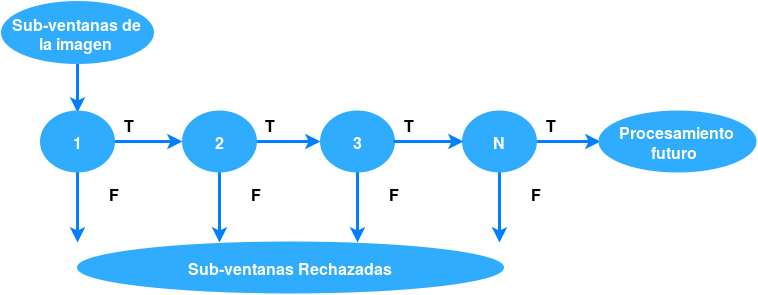
\includegraphics[scale=.60]{./Figures/DCascade.png}
\end{center}
\caption{Proceso del clasificador en forma de cascada, donde F representa la tasa de falsos positivos del clasificador de cascada y T representa el n\'umero de características.}
\label{fig:Cascade}
\end{figure}

El proceso de detección funciona de la siguiente manera: la sub-ventana es evaluada en el primer clasificador; un resultado positivo desencadena la evaluación de un segundo clasificador, el cual también ha sido ajustado para alcanzar cierta precisión; un resultado positivo en el segundo clasificador desencadena una tercera evaluación en el siguiente clasificador y así sucesivamente. Un resultado negativo en cualquier punto del proceso de evaluación conduce al rechazo inmediato de la sub-ventana.

La tasa de detección del clasificador en forma de cascada es: 
\begin{equation} \label{eq:D}
D = \prod^K_{i=1} d_i ,
\end{equation}
donde $d_i$ es la tasa de precisión de detección del $i$-ésimo clasificador fuerte.  

La tasa de precisión de falsos positivos, $F$ del clasificador de cascada es: 
\begin{equation} \label{eq:F}
F = \prod^K_{i=1} f_i ,
\end{equation}
donde $K$ es el número de clasificadores fuertes y $f_i$ es la tasa de precisión del $i$-ésimo clasificador. 
 
El algoritmo para calcular el clasificador en forma de cascada se encuentra en el Apéndice \ref{capit:apendB}. 

\subsection{Binarización}\label{subsec:Binarization} 

La binarización es una técnica de procesamiento de imágenes la cual se encarga de transformar una imagen en escala de grises $S(x,y)$ en una imagen binaria $B(x,y)$. Es decir los pixeles de la imagen toman un valor de $0$ ó $1$. Para formar la imagen binaria un valor o umbral de la imagen en escala de grises es seleccionado. \\ 
Una vez seleccionado el umbral, $T$, los pixeles de la imagen son discriminados. Si el valor de los pixeles de la imagen es mayor o igual al umbral entonces el valor de los pixeles de la imagen binaria es $1$, si no toma el valor de $0$. Es decir: 
\begin{equation}
B(x,y)=
\begin{cases}   
1, \quad Si \quad S(x,y)\geq T \\
0, \quad de \quad otra \quad forma\\
\end{cases}.
\end{equation}

Existen diversas técnicas para binarizar una imagen, estas se pueden clasificar en dos grupos: global y local. Los métodos globales calculan un umbral el cual es utilizado para todos los pixeles de la imagen y los métodos locales que calculan varios umbrales para ciertas regiones de la imagen \citep{Chaki2014}.  En este trabajo se utiliza el método desarrollado por \citep{Otsu1979}.

El técnica desarrolla por Otsu es un método de binarizaci\'on global. El algoritmo supone que existen dos clases de pixeles: los del fondo y los que representan el primer plano de la imagen. 

El método calcula el umbral optimo $T$ que separa a estas dos clases para el cual la varianza dentro las clases es la mínima. Para calcular $T$ que minimice las varianzas dentro de las clases, se define como una suma ponderada de las varianzas de las dos clases.
La varianza ponderada dentro de las clases es: 
\begin{equation}
\sigma^2_w(t) = q_1(t)\sigma^2_1(t) + q_2(t)\sigma^2_2(t),
\end{equation} 
donde las probabilidades de cada clase son calculadas mediante:  
\begin{equation}
q_1(t) = \sum ^t_{i=0} P(i) 
\qquad \text{y} \qquad
q_2(t) = \sum ^{255}_{i=t+1} P(i),
\end{equation} 
y la media de cada clase es calculada como:  
\begin{equation}
\mu_1(t) = \sum ^t_{i=0} \frac{i \cdot P(i)}{q_1(t)} 
\qquad \text{y} \qquad
\mu_2(t) = \sum ^{255}_{i=t+1} \frac{i \cdot P(i)}{q_2(t)}.
\end{equation} 
La varianza total $\sigma^2$, es igual a la suma de la varianza dentro de clase y la varianza entre clases $\sigma^2_b(t)$, es decir: 
\begin{equation}
\sigma^2 = \sigma^2_w(t) + \sigma^2_b(t),
\end{equation}
donde $\sigma^2_b(t)= q_1(t)\left[ 1- q_1(t) \right]\left[ \mu_1(t) - \mu_2(t) \right]^2 .$  
Como la varianza total no depende de $t$, es una constante, entonces para encontrar el umbral que minimice la varianza dentro de clases equivale a encontrar el máximo de $\sigma^2_b(t)$. 

\subsection{Operaciones Morfológicas}\label{subsec:OperacionesMorfologicas} 

Otra técnica muy utilizada en procesamiento de imágenes son las operaciones morfológicas. Que son un conjunto de operaciones no lineales. La idea es que al aplicar alguna de estas operaciones el ruido sea removido tomando en cuenta la forma y estructura de la imagen. 
Las operaciones morfológicas \citep{Premaratne2013} utilizan un elemento estructural el cual se aplica por toda la imagen. Los elementos estructurales pueden ser de distintas formas como los que se muestran en la Figura \ref{fig:EX}.
\begin{figure}[h!]
\centering
\subfigure[Rectángulo de $3x3$.]{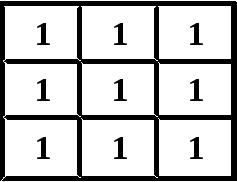
\includegraphics[scale=.68]{./Figures/EX1}\label{fig:EX:1}} \qquad
\subfigure[Figura de $3x2$.]{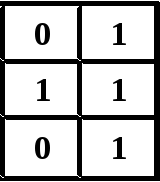
\includegraphics[scale=.68]{./Figures/EX3}\label{fig:EX:3}} \qquad
\subfigure[Cruz de $5x5$.]{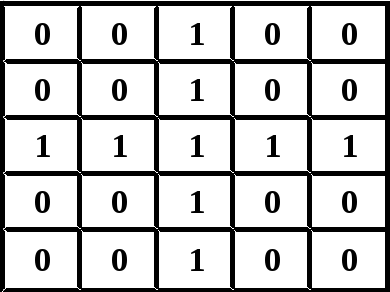
\includegraphics[scale=.42]{./Figures/EX2}\label{fig:EX:2}} 
\caption{Ejemplos de elementos estructurales.} \label{fig:EX}
\end{figure} 

Existen distintas operaciones morfológicas, las básicas o principales son la dilatación y erosión las cuales se explican enseguida junto con la apertura y cierre. 
 
\subsubsection{Dilatación}\label{sssec:Dilatation}
La dilatación es una operación que añade pixeles a la orilla de los objetos que se encuentran en la imagen. En la Figura \ref{fig:OM:2} 
se aplica esta operación a la Figura \ref{fig:OM:1}.
La dilatación se define como:  
\begin{equation}
S \oplus EX = \lbrace S|EX_S \subseteq S \rbrace,
\end{equation}
donde $EX_S$ es el elemento estructural trasladado con la imagen. 

\subsubsection{Erosión}\label{sssec:OMerosion}
La erosión remueve pixeles a la orilla de los objetos que se encuentran en la imagen. En la Figura \ref{fig:OM:3} se muestra el resultado de aplicar la operación a la Figura \ref{fig:OM:1}.
La erosión se define como: 
\begin{equation}
S \ominus EX = \lbrace S|EX_S \subseteq S \rbrace,
\end{equation}
donde $EX_S$ es el elemento estructural trasladado con la imagen. 

\subsubsection{Apertura}\label{sssec:Opening} 
La operación apertura abre huecos entre objetos conectados por un enlace delgado de pixeles, también suaviza los contornos del objeto. Esta operación es calculada realizando dos operaciones básicas: una erosión seguida de una dilatación. 
La apertura se define como:  
\begin{equation}
S \circ EX = (S \ominus EX) \oplus EX.
\end{equation}
La Figura \ref{fig:OM:4} muestra el resultado de aplicar la operación apertura a la Figura \ref{fig:OM:1}.

\subsubsection{Cierre}\label{sssec:Closure}
La operación cierre elimina huecos pequeños y rellena huecos en los contornos. El cierre es calculado realizando las operación de dilatación seguida de la erosión.
El cierre se define como:
\begin{equation}
S \bullet EX = (S \oplus EX) \ominus EX.
\end{equation}
La Figura \ref{fig:OM:5} muestra el resultado de aplicar la operación a la Figura \ref{fig:OM:1}.

\begin{figure}[h!]
\centering
\subfigure[original]{
\includegraphics[scale=.55]{./Figures/originalMO}\label{fig:OM:1}} \hspace{10mm}
\subfigure[dilatación]{
\includegraphics[scale=.55]{./Figures/dilatationMO}\label{fig:OM:2}} \hspace{10mm}
\subfigure[erosión]{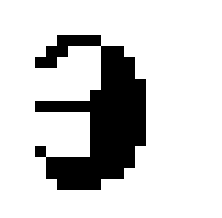
\includegraphics[scale=.55]{./Figures/erosionMO}\label{fig:OM:3}} \hspace{10mm}
\subfigure[apertura]{
\includegraphics[scale=.55]{./Figures/openingMO}\label{fig:OM:4}} \hspace{10mm}
\subfigure[cierre]{
\includegraphics[scale=.55]{./Figures/closingMO}\label{fig:OM:5}}
\caption{Aplicación de las principales operaciones morfológicas a la imagen que se encuentra en el inciso a), \protect\citep{Smith1999} } \label{fig:OM}
\end{figure} 


%:::::::::::::::::::::::::::::::::::::::::::::::::::::::::::::::::::::::::::::::::::::::::::::::::::::::::::::::::::::::::::::::::::


\section{Extracción de características}\label{sec:Convexhull} 

La finalidad de esta etapa es obtener las características de la imagen que sean capaces de describir la mano, de manera que con estas, se pueda reconocer los gestos realizados.
   
En este trabajo se extraen características geométricas, las cuales son extraídas de la siguiente forma, ver Figura \ref{fig:DiagramaExtraccionCaracteristicas}: el primer paso es encontrar la envolvente convexa de la mano para posteriormente calcular los defectos de convexidad, una vez aplicados estos algoritmos se calcula el número de dedos de la mano entre otras características; finalmente las características calculadas  se guardan en un vector.  

\begin{figure}[h!]
\begin{center}
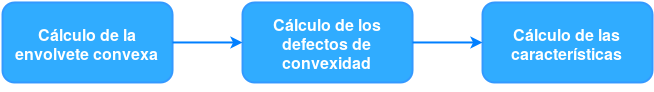
\includegraphics[scale=.7]{./Figures/DExtraccion.png}
\end{center}
\caption{Proceso de la extracción de características.}
\label{fig:DiagramaExtraccionCaracteristicas}
\end{figure} 

A continuación se definen los conceptos anteriores y el de conjunto convexo.

Sea $A$ un conjunto en el espacio euclidiano $\bold{\Re}^d$, donde $d$ es la dimensión del espacio euclidiano. $A$ es un conjunto convexo \footnote{\label{ConvexFN} Weisstein, Eric W. "Convex." From MathWorld--A Wolfram Web Resource. \url{http://mathworld.wolfram.com/Convex.html}} si contiene todos los segmentos de línea que unen a cualquier par de puntos pertenecientes al conjunto.  
\begin{figure}[h!]
\centering
\subfigure[Convexo]{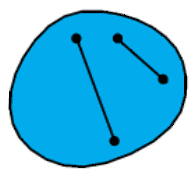
\includegraphics[scale=.8]{./Figures/ConvexSet.png}\label{fig:Sets:Convex}} \hspace{10mm}
\subfigure[conexo]{
\includegraphics[scale=.75]{./Figures/ConcaveSet.png}\label{fig:OM:Concave}} \hspace{10mm}
\caption{Ejemplo de un conjunto conexo y un convexo. Image recuperada de \ref{ConvexFN} }\label{fig:Sets}
\end{figure} 

Sea $B$ un conjunto de puntos en el plano Euclidiano, la envolvente convexa de $B$ es el conjunto convexo más pequeño que contiene a todos los puntos en $B$. En la Figura \ref{fig:FigConvexHullDefects} se muestra de color rojo la envolvente convexa de la Figura cuyo contorno se encuentra de color negro. 

Los defectos de convexidad de la envolvente convexa, son el conjunto de puntos que no pertenecen a la envolvente convexa. El defecto es el espacio que existe entre el contorno de la envolvente convexa y del objeto.

Sea $CD=\lbrace cd_1, cd_2, \cdots, cd_n \rbrace$ el conjunto de defectos de convexidad de una envolvente convexa. Cada defecto está compuesto por tres elementos: el punto de inicio del defecto $s_i(x,y)$, el punto con mayor distancia de la envolvente al objeto, $d_i(x,y)$ y el punto final del defecto, $e_i(x,y)$.
En la Figura \ref{fig:FigConvexHullDefects} los puntos amarillos representan los puntos de profundidad de los defectos de convexidad. 

\begin{figure}[h!]
\begin{center}
\includegraphics[scale=.4]{./Figures/ConvexHullAndDefects.png}
\end{center}
\caption{En la imagen se aprecia de color rojo la envolvente convexa, de negro el contorno de la figura y los puntos amarillos son el punto de profundidad de los defectos de convexidad.}
\label{fig:FigConvexHullDefects}
\end{figure}  

Usando las técnicas anteriores podemos extraer características importantes como el número de dedos, la posición del centro de la palma de mano, la posición de la punta de los dedos, la posición del inicio o raíz de los dedos, el ángulo del centro de la palma de la mano a la punta de los dedos, ángulo $TC$, el ángulo del centro de la palma de la mano al inicio de los dedos, ángulo $RC$ y la distancia vertical del centro de la palma de la mano al inicio de los dedos. Enseguida se explica cómo son obtenidas las características mencionadas. 

El número de dedos que se encuentran levantados es calculado con el Algoritmo \ref{alg:NumDedos} desarrollado por \citep{Kathuria2011}, ver Apéndice \ref{capit:apendC}, el cual utiliza los defectos de convexidad en especifico los conjuntos de puntos de inicio, $\mathcal{S}=\lbrace s_1(x,y), s_2(x,y), \cdots, s_n(x,y) \rbrace$, los puntos de mayor distancia, $\mathcal{D}=\lbrace d_1(x,y), d_2(x,y), \cdots, d_n(x,y) \rbrace$, las distancias del punto de inicio al de mayor distancia, $\mathcal{\delta}=\lbrace \delta_1(x,y), \delta_2(x,y), \cdots, \delta_n(x,y) \rbrace$, donde $n$ es el número total de defectos de la envolvente convexa.
Sea $C_r(x,y)$, el punto que representa el centroide del rectángulo más pequeño que encierra a la mano, $L_r$, la altura del rectángulo y $k$ una constante. 

La posición de la raíz de los dedos, $Fr(s,y)$ puede ser calculada usando los defectos de convexidad \citep{Hummel2014}, en especifico los puntos de profundidad, $d(x,y)$. Se calcula tomando el punto medio de los puntos de profundidad consecutivos encontrados en medio de los dedos, como se muestra en la Figura \ref{fig:RootFingers} . Es decir: 
\begin{equation}
Fr_i(x,y)= \left( \frac{ x_{d_i}+x_{d_{i-1}} }{2},\frac{y_{d_i}+y_{d_{i-1}}}{2}  \right),
\end{equation}
donde $i$ representa el número de dedo, cuando $i=0$ se toma el punto de profundidad anterior al dedo, si $i=6$ se toma el punto de profundidad posterior al dedo. 

\begin{figure}[h!]
\begin{center}
\includegraphics[scale=.55]{./Figures/rootFingers.png}
\end{center}
\caption{La figura muestra parte de la mano y en ella se aprecia los siguientes elementos: en color rojo la envolvente convexa, en amarillo los puntos de inicio y final de los defectos de convexidad,  en color azul los puntos de profundidad de los defectos, en verde la linea que une a los puntos de profundidad consecutivos y finalmente en morado los puntos medios, \protect\citep{Hummel2014}} 
\label{fig:RootFingers}
\end{figure} 

El centro de la palma de mano también se calcula, con los puntos de profundidad de los defectos de convexidad. Se toma como centro de la palma de la mano el centro del rectángulo más chico que une rodea a los puntos de convexidad. 

El ángulo $RC$ es el formado por el eje $y$  y la línea que une al punto que representa la posición de la raíz de los dedos, $Fr(x,y)$ con el centro de la palma de la mano, $Ch(x,y)$, \citep{Sgouropoulos2014}. 
\begin{equation}
\angle RC = 90^\circ - \tan^{-1} \left( \frac{ y_{Fr}-y_{Ch} }{ x_{Fr}-x_{Ch} } \right).
\end{equation}


El ángulo $TC$ es el formado por el eje $y$ y la línea que une al centro de la mano, $Ch(x,y)$ y con el de la punta de los dedos, $Ft(x,y)$, \citep{Sgouropoulos2014}. El  ángulo anterior se representa como:
\begin{equation}
\angle TC = 90^\circ - \tan^{-1} \left( \frac{ y_{Ft}-y_{Ch} }{ x_{Ft}-x_{Ch} } \right).
\end{equation}
 

La distancia $PC$ es la distancia vertical de la raíz del dedo al centro de la palma de la mano. Esta distancia es invariante al tamaño de la mano ya que es dividida por el tamaño de la palma, que se toma como el ancho del rectángulo que encierra la palma.  

\begin{figure}[h!]
\begin{center}
\includegraphics[scale=.6]{./Figures/angles.png}
\end{center}
\caption{En la imagen se representan los siguientes elementos, el eje vertical con respecto a la mano se encuentra como una línea de color verde; la línea roja represente la distancia del eje vertical a la raíz de los dedos; el punto rosa representa el centro de la palma de la mano, el área azul representa el ángulo de que existe de la línea que une al centro con la raíz de los dedos y finalmente el área anaranjada representa el ángulo que forma la línea del centro a la punta de los dedos, \protect\citep{Sgouropoulos2014}.}
\label{fig:anglesFingers}
\end{figure} 


Una vez que todas las características son calculadas estas son guardadas en un vector, llamado vector de características. La dimensión del vector es el número de características que este contiene. 


%:::::::::::::::::::::::::::::::::::::::::::::::::::::::::::::::::::::::::::::::::::::::::::::::::::::::::::::::::::::::::::::::::


\section{Reconocimiento}\label{sec:SVM} 

Es la etapa final del reconocimiento, es donde el gesto realizado por el usuario finalmente puede ser interpretado por la computadora.
En este trabajo el reconocimiento se realiza utilizando el algoritmo de máquinas de soporte vectorial SVM, por sus siglas en ingl\'es \citep{Cortes1995}, un método de aprendizaje de máquina supervisado el cual es utilizado para resolver problemas de clasificación y regresión. SVM tiene como objetivo crear un modelo basado en datos conocidos, datos de entrenamiento, donde este modelo es capaz de predecir a que clase pertenecen datos nuevos. 

SVM realiza la clasificación separando las clases calculando el hiperplano que tengan el margen de separación más grande. En la Figura \ref{fig:SVM} se muestra en conjunto de clases separables por medio de un hiperplano.  

\begin{figure}[h!]
\begin{center}
\includegraphics[scale=.55]{./Figures/SVMarticle.png}
\end{center}
\caption{La imagen muestra la separación de dos clases, (los círculos en color azul y negro), mediante un hiperplano óptimo; donde $\text{w}$ representa la normal al hiperplano, $\frac{\textbf{-b}}{\textbf{\text{w}}}$ la distancia el hiperplano al origen \protect\citep{Burges1998}.}
\label{fig:SVM}
\end{figure} 

Enseguida se explica el caso cuando las clases son linealmente separables.

Dado $N$ muestras de entrenamiento $x_i$, de dimensión $D$, dos clases distintas $y_i=-1$ ó $+1$ es decir: 
$$\lbrace x_i,y_i \rbrace \quad \text{donde} \quad  i=1, \cdots ,N \quad y\in \lbrace -1,1 \rbrace \quad x \in \Re^D.$$
Sea  
\begin{equation}\label{eq:hiper}
\text{w} \cdot x + \text{b} = 0 ,
\end{equation}  
el hiperplano óptimo que separa a las clases, donde $\text{w}$ es la normal al hiperplano, $\frac{\text{b}}{ \Vert \text{w} \Vert}$ es la distancia perpendicular desde el hiperplano al origen.

Sea $d_+$, la menor distancia del hiperplano que separa a las muestras positivas de las negativas y $d_-$, la menor distancia del hiperplano que separa a las muestras negativas de las positivas. Se define el margen del hiperplano como la suma de estas distancias, es decir: $d_+ + d_-$.

Para el caso cuando las clases son linealmente separables basta con encontrar el hiperplano con el margen mayor. Es decir que el hiperplano puede ser calculado seleccionando $\text{w}$ y $\text{b}$ de manera que los datos de entrenamiento cumplan con:  
\begin{equation}\label{eq:des+1}
\text{w} \cdot x_i + \text{b} \geqslant +1 \quad \textrm{ para } \quad y_i=+1
\end{equation} 
\begin{equation}\label{eq:des-1}
\text{w} \cdot x_i + \text{b} \leqslant -1 \quad \textrm{ para } \quad y_i=-1
\end{equation} 
Combinando las desigualdades anteriores, se obtiene:  
\begin{equation}
y_i(x_i \cdot \text{w} + \text{b}) -1 \geqslant 0 \qquad \forall i 
\end{equation} 

Tomando en cuenta los puntos en donde se cumple la igualdad de la Ecuación \ref{eq:des+1}. Estos puntos se encuentran sobre el hiperplano $H_1$, el cual se escribe como: 
\begin{equation}\label{eq:eq+1}
\text{w} \cdot x_i + \text{b} = +1,  
\end{equation} 
con normal $\text{w}$ y una distancia perpendicular desde el origen de $\frac{\vert 1-\text{b} \vert}{ \Vert \text{w} \Vert}$. 
Similarmente para la Ecuación \ref{eq:des-1}, entonces el hiperplano $H_2$ se describe como: 
\begin{equation}\label{eq:eq+1}
\text{w} \cdot x_i + \text{b} = -1,  
\end{equation} 
con normal $\text{w}$ y una distancia perpendicular desde el origen de $\frac{\vert-1-\text{b}\vert}{ \Vert \text{w} \Vert}$.
Como $d_+ = d_- = \frac{1}{\Vert \text{w} \Vert}$, el margen es $\frac{2}{\Vert \text{w} \Vert}$. Los hiperplanos son paralelos pues tienen la misma normal, también ninguna muestra de entrenamiento caen entre ellos. Entonces se puede encontrar un par de hiperplanos  que tengan un margen máximo minimizando $\Vert \text{w} \Vert^2$, es decir:  
\begin{equation}
\text{min} \quad \frac{1}{2} \Vert \text{w} \Vert \quad \text{tal que} \quad y_i(\text{w} \cdot x_i + \text{b}) -1 \geq 0.
\end{equation}  


\newpage
%%=====================================================
} }%
%BeginExpansion
\chapter{Sistema propuesto de reconocimiento de gestos}\label{capit:cap3}
\vspace{-2.0325ex}%
\noindent
\rule{\textwidth}{0.5pt}
\vspace{-5.5ex}% 
\newcommand{\pushline}{\Indp}% Indent puede ir o no :p 

En este cap\'itulo se describen las etapas del sistema propuesto junto con los métodos y algoritmos que son utilizados en cada una de las fases.
 
El sistema propuesto de reconocimiento de gestos consta de cuatro etapas principales, Figura \ref{fig:MyHGR}. La primera etapa es la adquisición de los datos, en la cual se capturan las imágenes de entrada del sistema. La siguiente etapa es la detección, aquí la mano es localizada y segmentada del fondo. En la etapa tres se extraen las características de la mano para ser procesadas. En la etapa final el gesto realizado es reconocido.   

\begin{figure}[h!]
\begin{center}
\includegraphics[scale=.6]{./Figures/MyHGR.png}
\end{center}
\caption{Metodología del sistema propuesto.}
\label{fig:MyHGR}
\end{figure}  
  
\section{Adquisición de los datos}\label{sec:KinectSensor} 

En la primera etapa del sistema los datos de entrada del sistema son capturados y preprocesados, la Figura \ref{fig:Dadquisicion} muestra las etapas de este proceso. Los datos provienen de los sensores de profundidad de dos dispositivos Kinect. Debido a la naturaleza del sensor las imágenes capturadas contiene ruido por interferencia \citep{Mallick2014}, que puede ser reducido utilizando filtro de medianas \citep{Maimone2011}.

\begin{figure}[h!]
\begin{center}
\includegraphics[scale=.6]{./Figures/Adquisicion.png}
\end{center}
\caption{Proceso de la etapa de adquisición de datos.} 
\label{fig:Dadquisicion}
\end{figure}   


\subsection{Kinect}

En noviembre del 2010 la compa\'nia Microsoft lanz\'o el sensor Kinect para consolas de vídeo juego Xbox 360 y en febrero del 2011 lanz\'o la versi\'on para Windows. El dispositivo fue desarrollado por la compa\~nia PrimeSense en conjunto con Microsoft \footnote{\url{engadget.com/2013/06/21/life-after-kinect-primesense-post-microsoft/}}. El sensor de profundidad que utiliza el dispositivo fue desarrollado por Zeev Zalesvky, Alexanser Shpunt, Aviad Maizels y Javier Garcia en 2005 \footnote{\url{https://patentscope.wipo.int/search/en/detail.jsf?docId=WO2007043036&recNum=1&maxRec=&office=&prevFilter=&sortOption=&queryString=&tab=PCT+Biblio}}   


El dispositivo Kinect está equipado con una serie de sensores que permiten obtener imágenes a color y de profundidad (las cuales indican la distancia a la que está ubicada un objeto del sensor). La Figura \ref{fig:KinectPic} muestra la parte frontal del dispositivo Kinect para Windows. Los sensores permiten hacer detección y seguimiento de personas. El dispositivo tiene la capacidad de detectar hasta seis personas y hacer el seguimiento de hasta dos personas \footnote{\url{https://msdn.microsoft.com/en-us/library/hh973074.aspx}}.    
  
\begin{figure}[h!]
\begin{center}
\includegraphics[scale=.65]{./Figures/Kinect.jpg}
\end{center}
\caption{Parte frontal del dispositivo Kinect en su versión para Windows, imagen recuperada de \protect\footnotemark{}.} 
\label{fig:KinectPic}
\end{figure} 

\footnotetext{\url{http://goo.gl/2GlwI}}

El sensor está equipado con los siguientes componentes: un cámara de color (o sensor de color), un emisor infrarrojo, un sensor infrarrojo de profundidad, un motor que controla la inclinación, un arreglo de cuatro micrófonos y un LED \citep{Jana2013}.
Enseguida se describen brevemente cada uno de los componentes del sensor Kinect, estos se muestran en la Figura \ref{fig:KinectComponentes}. 

\begin{figure}[h!]
\begin{center}
\includegraphics[scale=.6]{./Figures/sensor.png}
\end{center}
\caption{Componentes del sensor Kinect, imagen recuperada de \footnotemark{}.} 
\label{fig:KinectComponentes}
\end{figure}   

\footnotetext{\url{https://msdn.microsoft.com/en-us/library/jj131033.aspx}}

\begin{itemize}
\item La cámara de color captura y transmite datos de vídeo a color, detectando los colores rojo, verde y azul (RGB, por sus siglas en ingl\'es, red, green and blue). La transmisión de datos que brinda la cámara es una secuencia de imágenes (cuadros), a una velocidad de hasta treinta cuadros por segundo con una resolución de hasta $1280\, x \, 960$ p\'ixeles. La velocidad de los cuadros por segundo varia según la resolución de la imagen.

\item El emisor infrarrojo proyecta puntos de luz infrarroja, estos puntos son proyectados frente al sensor. Estos puntos junto con el sensor de profundidad es posible medir la distancia que existe del sensor a algún objeto que esté frente a él.  

\item El sensor infrarrojo lee los puntos infrarrojos proyectados por el emisor infrarrojo, con la lectura de los datos se calcula la distancia que existe entre el objeto y el sensor. El sensor transmite los datos de profundidad con una velocidad de hasta treinta cuadros por segundo con una resolución de hasta $640 \, x \, 480$ pixeles.   

\item El motor de inclinación controla el \'angulo de la posición vertical de los sensores del dispositivo. El motor puede moverse desde un \'angulo de $-27^ \circ$ a $+27^\circ$, con respecto al eje vertical del sensor.  

\item La entrada de audio compuesta por un arreglo de cuatro micrófonos permite capturar el sonido y calcular la posición de la fuente.

\item LED indica el estado del sensor. El LED en color verde indica que el sensor está disponible para utilizarse. El LED en color rojo indica que no existe conexión entre el Kinect y la computadora. La ausencia de color en el LED indica que el Kinect no se encuentra conectado a la fuente de energía eléctrica.
\end{itemize}

\subsection{Filtro de mediana} 

Existen distintos métodos para eliminar el ruido por interferencia causado por dos o más  Kinect, algunos de estos métodos son invasivos pues el hardware del Kinect es modificado \citep{Mallick2014}. Una opción es utilizar filtro de mediana, debido a que rellena los valores faltantes en la imagen proveniente del Kinect \citep{Maimone2011}. 

Sea $W_{mn}$ el vecindario de tamaño $m \times n$, centrado en el pixel, $s$, que se encuentra en la posición $(x,y)$. El filtro de mediana de la imagen $S(x,y)$, se calcula como: 
\begin{equation}
s(x,y)=\underset{(u,v)\in W_{mn}}{\text{mediana}} \lbrace S(u,v)\rbrace
\end{equation}

El filtro de mediana reemplaza el valor del pixel usando la mediana de las intensidades del vecindario del pixel, el valor del pixel en la posición (x,y) es incluido en el calculo \citep{Gonzalez2002}. 
 

%:::::::::::::::::::::::::::::::::::::::::::::::::::::::::::::::::::::::::::::::::::::::::::::::::::::::::::::::::::::::::::::::::::::::


\section{Detección}\label{sec:Detection}

En esta etapa del sistema el objetivo es localizar la mano en la imagen y segmentar la mano del fondo de la imagen. Para extraer las características necesarias para el reconocimiento.
La Figura \ref{fig:ProcesoDeteccion} muestra el proceso para  realizar la etapa de detección. El primer paso es localizar la mano, en este trabajo se utiliza el método de detección rápida de objetos; el siguiente paso es segmentar la mano del fondo, binarizando la imagen de la mano usando el algoritmo propuesto por \citep{Otsu1979}; finalmente se aplican las operaciones morfológicas apertura y cierre, para mejorar la segmentación, es decir eliminar ruido existente. 

\begin{figure}[h!]
\begin{center}
\includegraphics[scale=.7]{./Figures/Detection.png}
\end{center}
\caption{Proceso de detección de la mano.}
\label{fig:ProcesoDeteccion}
\end{figure} 

\subsection{Método detección rápida de objetos usando características simples utilizando el clasificador AdaBoost en forma de cascada}\label{subsec:ViolaJones}

En este trabajo se utiliza el método detección rápida de objetos usando características simples utilizando el clasificador AdaBoost en forma de cascada propuesto por \citep{Viola2001}, el cual fue creado originalmente para atacar el problema de detección de rostros. El método puede ser usando para detectar cualquier objeto debido a que la detección se realiza clasificando imágenes basándose en el valor de características simples.

La técnica detecta si el objeto se encuentra en la escena, usando una versión modificada del clasificador AdaBoost \citep{Freund1995} en forma de cascada y discrimina el objeto tomando en cuenta el valor de las características Haar \citep{Viola2001}. Las características son seleccionadas usando también el clasificador AdaBoost y el valor de éstas es calculado mediante el uso de una imagen integral \citep{Viola2001}. 

La Figura \ref{fig:ViolaJonesDiagram} muestra un diagrama del proceso del método de detección, el primer paso es obtener la muestras de entrenamiento con las cuales se construirá el clasificador; el siguiente paso es seleccionar las características que formarán el clasificador. Estas se escogen mediante el algoritmo de AdaBoost y su valor es calculado usando la imagen integral. El paso final  involucra construir el clasificador mediante el uso de Adaboost,  en forma de cascada.

\begin{figure}[h!]
\begin{center}
\includegraphics[scale=.6]{./Figures/ViolaJonesDiagram.png}
\end{center}
\caption{Procedimiento del algoritmo de detección rápida de objetos.}
\label{fig:ViolaJonesDiagram}
\end{figure}

Enseguida se explica a detalle cada etapa del método \citep{Viola2001}. 

\subsubsection{Características Haar}\label{sssec:CaracteristicasHaar}  

Las características Haar, son operadores rectangulares como los que se muestran en la Figura \ref{fig:haarFeatures}. A continuación se explicarán los operadores Haar básicos:
\begin{itemize}
\item Las características con dos rectángulos Figura \ref{fig:haarFeatures:1}, Figura \ref{fig:haarFeatures:2}, contienen dos regiones rectangulares adyacentes, el valor de la característica se calcula tomando la diferencia de la suma de ambas regiones. 

\item Las características con tres rectángulos Figura \ref{fig:haarFeatures:3}, contienen tres regiones rectangulares adyacentes, el valor de la característica se calcula sumando las regiones exteriores y restando la suma de la región interior.

\item Las características con cuatro rectángulos Figura \ref{fig:haarFeatures:4}, contienen cuatro regiones rectangulares adyacentes, el valor de la característica se obtiene con la diferencia entre la suma de las regiones pares diagonales.
\end{itemize} 

\begin{figure}[h!]
\centering
\subfigure[]{\includegraphics[scale=.4]{./Figures/haarFeatures1}\label{fig:haarFeatures:1}}
\subfigure[]{\includegraphics[scale=.4]{./Figures/haarFeatures2}\label{fig:haarFeatures:2}}
\subfigure[]{\includegraphics[scale=.4]{./Figures/haarFeatures3}\label{fig:haarFeatures:3}}
\subfigure[]{\includegraphics[scale=.4]{./Figures/haarFeatures4}\label{fig:haarFeatures:4}}
\caption{Ejemplo de tipos de operadores Haar.} \label{fig:haarFeatures}
\end{figure}


\subsubsection{Imagen integral}\label{sssec:IntegralImage} 

Uno de los aportes del método desarrollado por Viola y Jones es el concepto de imagen integral con la cual se calcula el valor de las características de manera rápida, es decir en tiempo constante, $O(1)$.  

La imagen integral, $SI$, de una imagen, $S(x,y)$, es calculada como la suma del valor de los pixeles que se encuentran arriba y a la izquierda de cierta posición de la imagen a la cual se le quiere hacer el cálculo. Lo anterior se puede escribir como: \footnote{\url{https://goo.gl/0oIJBz}}   
\begin{equation}
SI(x,y)=S(x,y) + S(x-1,y) + SI(x,y-1)-SI(x-1,y-1).
\end{equation}   
La Figura \ref{fig:FigIntegralImage} muestra un  ejemplo donde se calcula la imagen integral, Figura \ref{fig:FigIntegralImage:2}, de la imagen original Figura \ref{fig:FigIntegralImage:1}.
\begin{figure}[h!]
\centering
\subfigure[Imagen original]{\includegraphics[scale=.6]{./Figures/ImagetoIntegral}\label{fig:FigIntegralImage:1}} \qquad
\subfigure[Imagen integral]{\includegraphics[scale=.6]{./Figures/CalculationIntegral}\label{fig:FigIntegralImage:2}}
\caption{Ejemplo del cálculo de la imagen integral.} 
\label{fig:FigIntegralImage}
\end{figure}

La imagen integral permite calcular la suma de los pixeles de cierta región usando solo los valores de las esquinas de la imagen integral de dicha región, la cual se obtiene como: \footnote{\url{https://goo.gl/0oIJBz}}    
\begin{equation}
REG(\alpha)=SI(A)+SI(D)-SI(B)-SI(C),
\end{equation}
donde $REG(\alpha)$ es la región a la cual se quiere calcular el valor de la suma de sus pixeles; $A,B,C,D$ son las esquinas de dicha región. Como se muestra en la Figura \ref{fig:figImageIntegral}, la región $\alpha$ se encuentra resaltada en color azul.  
\begin{figure}[h!]
\begin{center}
\includegraphics[scale=.25]{./Figures/IntegralImage.png}
\end{center}
\caption{Regiones de la imagen integral.}
\label{fig:figImageIntegral}
\end{figure} 


\subsubsection{Algoritmo AdaBoost}\label{sssec:AdaboostClasifier}  

En el método de detección el clasificador AdaBoost es utilizado para seleccionar las características relevantes, con las cuales se podrá detectar el objeto. También es utilizado para construir el clasificador final pero en forma de cascada, el cual es explicado en la sección \ref{sssec:AdaboostCascade}. 

El algoritmo AdaBoost realiza la discriminación de objetos construyendo un clasificador fuerte, $h(x)$, llamado así debido a que tiene una precisión mayor en comparación con los clasificadores con los que es construido, clasificadores débiles, $h_i(x)$. Los clasificadores débiles son calculados de la siguiente manera: 
\begin{equation}
h_i(x)=
\begin{cases}   
1, \quad si \quad  p_if_i(x)<p_i \theta_i \\
0, \quad de \quad otra \quad forma.\\
\end{cases} ,
\end{equation}
donde $x$ es una sub-ventana de la imagen, $f_i(x)$ es una característica, $\theta$ es un umbral, y $p_i$ representa el signo de la desigualdad.   

El clasificador fuerte es una combinación lineal de los clasificadores débiles, y se define de la siguiente forma: 
\begin{equation}
h(x)= \alpha_1h_1(x)+\alpha_2h_2(x)+ \cdots +\alpha_nh_n(x) ,
\end{equation}
donde $n$ es el n\'umero de características, $\alpha_i$ es el valor asociado a cada característica, el cual va entre $0$ y $1$. En el Apéndice \ref{capit:apendA} se encuentra el algoritmo para calcular el clasificador fuerte.

\subsubsection{Clasificador AdaBoost en cascada}\label{sssec:AdaboostCascade}   

El objetivo de realizar la detección utilizando un clasificador en forma de cascada es descartar de manera rápida las regiones donde no se encuentra el objeto.

El clasificador en cascada está compuesto por etapas Figura \ref{fig:Cascade}, cada una de estas es un clasificador fuerte. Este clasificador es entrenado por medio de AdaBoost. El cual se encarga de encontrar el orden de evaluación de las características relevantes. 
La selección se realiza como se muestra en el Algoritmo \ref{alg:Cascade}, cumpliendo cierta precisión en la detección $D$, ver Ecuación \ref{eq:D}, cierta tasa de falsos positivos $F$, ver Ecuación \ref{eq:F} .

\begin{figure}[h!]
\begin{center}
\includegraphics[scale=.60]{./Figures/DCascade.png}
\end{center}
\caption{Proceso del clasificador en forma de cascada, donde F representa la tasa de falsos positivos del clasificador de cascada y T representa el n\'umero de características.}
\label{fig:Cascade}
\end{figure}

El proceso de detección funciona de la siguiente manera: la sub-ventana es evaluada en el primer clasificador; un resultado positivo desencadena la evaluación de un segundo clasificador, el cual también ha sido ajustado para alcanzar cierta precisión; un resultado positivo en el segundo clasificador desencadena una tercera evaluación en el siguiente clasificador y así sucesivamente. Un resultado negativo en cualquier punto del proceso de evaluación conduce al rechazo inmediato de la sub-ventana.

La tasa de detección del clasificador en forma de cascada es: 
\begin{equation} \label{eq:D}
D = \prod^K_{i=1} d_i ,
\end{equation}
donde $d_i$ es la tasa de precisión de detección del $i$-ésimo clasificador fuerte.  

La tasa de precisión de falsos positivos, $F$ del clasificador de cascada es: 
\begin{equation} \label{eq:F}
F = \prod^K_{i=1} f_i ,
\end{equation}
donde $K$ es el número de clasificadores fuertes y $f_i$ es la tasa de precisión del $i$-ésimo clasificador. 
 
El algoritmo para calcular el clasificador en forma de cascada se encuentra en el Apéndice \ref{capit:apendB}. 

\subsection{Binarización}\label{subsec:Binarization} 

La binarización es una técnica de procesamiento de imágenes la cual se encarga de transformar una imagen en escala de grises $S(x,y)$ en una imagen binaria $B(x,y)$. Es decir los pixeles de la imagen toman un valor de $0$ ó $1$. Para formar la imagen binaria un valor o umbral de la imagen en escala de grises es seleccionado. \\ 
Una vez seleccionado el umbral, $T$, los pixeles de la imagen son discriminados. Si el valor de los pixeles de la imagen es mayor o igual al umbral entonces el valor de los pixeles de la imagen binaria es $1$, si no toma el valor de $0$. Es decir: 
\begin{equation}
B(x,y)=
\begin{cases}   
1, \quad Si \quad S(x,y)\geq T \\
0, \quad de \quad otra \quad forma\\
\end{cases}.
\end{equation}

Existen diversas técnicas para binarizar una imagen, estas se pueden clasificar en dos grupos: global y local. Los métodos globales calculan un umbral el cual es utilizado para todos los pixeles de la imagen y los métodos locales que calculan varios umbrales para ciertas regiones de la imagen \citep{Chaki2014}.  En este trabajo se utiliza el método desarrollado por \citep{Otsu1979}.

El técnica desarrolla por Otsu es un método de binarizaci\'on global. El algoritmo supone que existen dos clases de pixeles: los del fondo y los que representan el primer plano de la imagen. 

El método calcula el umbral optimo $T$ que separa a estas dos clases para el cual la varianza dentro las clases es la mínima. Para calcular $T$ que minimice las varianzas dentro de las clases, se define como una suma ponderada de las varianzas de las dos clases.
La varianza ponderada dentro de las clases es: 
\begin{equation}
\sigma^2_w(t) = q_1(t)\sigma^2_1(t) + q_2(t)\sigma^2_2(t),
\end{equation} 
donde las probabilidades de cada clase son calculadas mediante:  
\begin{equation}
q_1(t) = \sum ^t_{i=0} P(i) 
\qquad \text{y} \qquad
q_2(t) = \sum ^{255}_{i=t+1} P(i),
\end{equation} 
y la media de cada clase es calculada como:  
\begin{equation}
\mu_1(t) = \sum ^t_{i=0} \frac{i \cdot P(i)}{q_1(t)} 
\qquad \text{y} \qquad
\mu_2(t) = \sum ^{255}_{i=t+1} \frac{i \cdot P(i)}{q_2(t)}.
\end{equation} 
La varianza total $\sigma^2$, es igual a la suma de la varianza dentro de clase y la varianza entre clases $\sigma^2_b(t)$, es decir: 
\begin{equation}
\sigma^2 = \sigma^2_w(t) + \sigma^2_b(t),
\end{equation}
donde $\sigma^2_b(t)= q_1(t)\left[ 1- q_1(t) \right]\left[ \mu_1(t) - \mu_2(t) \right]^2 .$  
Como la varianza total no depende de $t$, es una constante, entonces para encontrar el umbral que minimice la varianza dentro de clases equivale a encontrar el máximo de $\sigma^2_b(t)$. 

\subsection{Operaciones Morfológicas}\label{subsec:OperacionesMorfologicas} 

Otra técnica muy utilizada en procesamiento de imágenes son las operaciones morfológicas. Que son un conjunto de operaciones no lineales. La idea es que al aplicar alguna de estas operaciones el ruido sea removido tomando en cuenta la forma y estructura de la imagen. 
Las operaciones morfológicas \citep{Premaratne2013} utilizan un elemento estructural el cual se aplica por toda la imagen. Los elementos estructurales pueden ser de distintas formas como los que se muestran en la Figura \ref{fig:EX}.
\begin{figure}[h!]
\centering
\subfigure[Rectángulo de $3x3$.]{\includegraphics[scale=.68]{./Figures/EX1}\label{fig:EX:1}} \qquad
\subfigure[Figura de $3x2$.]{\includegraphics[scale=.68]{./Figures/EX3}\label{fig:EX:3}} \qquad
\subfigure[Cruz de $5x5$.]{\includegraphics[scale=.42]{./Figures/EX2}\label{fig:EX:2}} 
\caption{Ejemplos de elementos estructurales.} \label{fig:EX}
\end{figure} 

Existen distintas operaciones morfológicas, las básicas o principales son la dilatación y erosión las cuales se explican enseguida junto con la apertura y cierre. 
 
\subsubsection{Dilatación}\label{sssec:Dilatation}
La dilatación es una operación que añade pixeles a la orilla de los objetos que se encuentran en la imagen. En la Figura \ref{fig:OM:2} 
se aplica esta operación a la Figura \ref{fig:OM:1}.
La dilatación se define como:  
\begin{equation}
S \oplus EX = \lbrace S|EX_S \subseteq S \rbrace,
\end{equation}
donde $EX_S$ es el elemento estructural trasladado con la imagen. 

\subsubsection{Erosión}\label{sssec:OMerosion}
La erosión remueve pixeles a la orilla de los objetos que se encuentran en la imagen. En la Figura \ref{fig:OM:3} se muestra el resultado de aplicar la operación a la Figura \ref{fig:OM:1}.
La erosión se define como: 
\begin{equation}
S \ominus EX = \lbrace S|EX_S \subseteq S \rbrace,
\end{equation}
donde $EX_S$ es el elemento estructural trasladado con la imagen. 

\subsubsection{Apertura}\label{sssec:Opening} 
La operación apertura abre huecos entre objetos conectados por un enlace delgado de pixeles, también suaviza los contornos del objeto. Esta operación es calculada realizando dos operaciones básicas: una erosión seguida de una dilatación. 
La apertura se define como:  
\begin{equation}
S \circ EX = (S \ominus EX) \oplus EX.
\end{equation}
La Figura \ref{fig:OM:4} muestra el resultado de aplicar la operación apertura a la Figura \ref{fig:OM:1}.

\subsubsection{Cierre}\label{sssec:Closure}
La operación cierre elimina huecos pequeños y rellena huecos en los contornos. El cierre es calculado realizando las operación de dilatación seguida de la erosión.
El cierre se define como:
\begin{equation}
S \bullet EX = (S \oplus EX) \ominus EX.
\end{equation}
La Figura \ref{fig:OM:5} muestra el resultado de aplicar la operación a la Figura \ref{fig:OM:1}.

\begin{figure}[h!]
\centering
\subfigure[original]{\includegraphics[scale=.55]{./Figures/originalMO}\label{fig:OM:1}} \hspace{10mm}
\subfigure[dilatación]{\includegraphics[scale=.55]{./Figures/dilatationMO}\label{fig:OM:2}} \hspace{10mm}
\subfigure[erosión]{\includegraphics[scale=.55]{./Figures/erosionMO}\label{fig:OM:3}} \hspace{10mm}
\subfigure[apertura]{\includegraphics[scale=.55]{./Figures/openingMO}\label{fig:OM:4}} \hspace{10mm}
\subfigure[cierre]{\includegraphics[scale=.55]{./Figures/closingMO}\label{fig:OM:5}}
\caption{Aplicación de las principales operaciones morfológicas a la imagen que se encuentra en el inciso a), \protect\citep{Smith1999} } \label{fig:OM}
\end{figure} 


%:::::::::::::::::::::::::::::::::::::::::::::::::::::::::::::::::::::::::::::::::::::::::::::::::::::::::::::::::::::::::::::::::::


\section{Extracción de características}\label{sec:Convexhull} 

La finalidad de esta etapa es obtener las características de la imagen que sean capaces de describir la mano, de manera que con estas, se pueda reconocer los gestos realizados.
   
En este trabajo se extraen características geométricas, las cuales son extraídas de la siguiente forma, ver Figura \ref{fig:DiagramaExtraccionCaracteristicas}: el primer paso es encontrar la envolvente convexa de la mano para posteriormente calcular los defectos de convexidad, una vez aplicados estos algoritmos se calcula el número de dedos de la mano entre otras características; finalmente las características calculadas  se guardan en un vector.  

\begin{figure}[h!]
\begin{center}
\includegraphics[scale=.7]{./Figures/DExtraccion.png}
\end{center}
\caption{Proceso de la extracción de características.}
\label{fig:DiagramaExtraccionCaracteristicas}
\end{figure} 

A continuación se definen los conceptos anteriores y el de conjunto convexo.

Sea $A$ un conjunto en el espacio euclidiano $\bold{\Re}^d$, donde $d$ es la dimensión del espacio euclidiano. $A$ es un conjunto convexo \footnote{\label{ConvexFN} Weisstein, Eric W. "Convex." From MathWorld--A Wolfram Web Resource. \url{http://mathworld.wolfram.com/Convex.html}} si contiene todos los segmentos de línea que unen a cualquier par de puntos pertenecientes al conjunto.  
\begin{figure}[h!]
\centering
\subfigure[Convexo]{\includegraphics[scale=.8]{./Figures/ConvexSet.png}\label{fig:Sets:Convex}} \hspace{10mm}
\subfigure[conexo]{\includegraphics[scale=.75]{./Figures/ConcaveSet.png}\label{fig:OM:Concave}} \hspace{10mm}
\caption{Ejemplo de un conjunto conexo y un convexo. Image recuperada de \ref{ConvexFN} }\label{fig:Sets}
\end{figure} 

Sea $B$ un conjunto de puntos en el plano Euclidiano, la envolvente convexa de $B$ es el conjunto convexo más pequeño que contiene a todos los puntos en $B$. En la Figura \ref{fig:FigConvexHullDefects} se muestra de color rojo la envolvente convexa de la Figura cuyo contorno se encuentra de color negro. 

Los defectos de convexidad de la envolvente convexa, son el conjunto de puntos que no pertenecen a la envolvente convexa. El defecto es el espacio que existe entre el contorno de la envolvente convexa y del objeto.

Sea $CD=\lbrace cd_1, cd_2, \cdots, cd_n \rbrace$ el conjunto de defectos de convexidad de una envolvente convexa. Cada defecto está compuesto por tres elementos: el punto de inicio del defecto $s_i(x,y)$, el punto con mayor distancia de la envolvente al objeto, $d_i(x,y)$ y el punto final del defecto, $e_i(x,y)$.
En la Figura \ref{fig:FigConvexHullDefects} los puntos amarillos representan los puntos de profundidad de los defectos de convexidad. 

\begin{figure}[h!]
\begin{center}
\includegraphics[scale=.4]{./Figures/ConvexHullAndDefects.png}
\end{center}
\caption{En la imagen se aprecia de color rojo la envolvente convexa, de negro el contorno de la figura y los puntos amarillos son el punto de profundidad de los defectos de convexidad.}
\label{fig:FigConvexHullDefects}
\end{figure}  

Usando las técnicas anteriores podemos extraer características importantes como el número de dedos, la posición del centro de la palma de mano, la posición de la punta de los dedos, la posición del inicio o raíz de los dedos, el ángulo del centro de la palma de la mano a la punta de los dedos, ángulo $TC$, el ángulo del centro de la palma de la mano al inicio de los dedos, ángulo $RC$ y la distancia vertical del centro de la palma de la mano al inicio de los dedos. Enseguida se explica cómo son obtenidas las características mencionadas. 

El número de dedos que se encuentran levantados es calculado con el Algoritmo \ref{alg:NumDedos} desarrollado por \citep{Kathuria2011}, ver Apéndice \ref{capit:apendC}, el cual utiliza los defectos de convexidad en especifico los conjuntos de puntos de inicio, $\mathcal{S}=\lbrace s_1(x,y), s_2(x,y), \cdots, s_n(x,y) \rbrace$, los puntos de mayor distancia, $\mathcal{D}=\lbrace d_1(x,y), d_2(x,y), \cdots, d_n(x,y) \rbrace$, las distancias del punto de inicio al de mayor distancia, $\mathcal{\delta}=\lbrace \delta_1(x,y), \delta_2(x,y), \cdots, \delta_n(x,y) \rbrace$, donde $n$ es el número total de defectos de la envolvente convexa.
Sea $C_r(x,y)$, el punto que representa el centroide del rectángulo más pequeño que encierra a la mano, $L_r$, la altura del rectángulo y $k$ una constante. 

La posición de la raíz de los dedos, $Fr(s,y)$ puede ser calculada usando los defectos de convexidad \citep{Hummel2014}, en especifico los puntos de profundidad, $d(x,y)$. Se calcula tomando el punto medio de los puntos de profundidad consecutivos encontrados en medio de los dedos, como se muestra en la Figura \ref{fig:RootFingers} . Es decir: 
\begin{equation}
Fr_i(x,y)= \left( \frac{ x_{d_i}+x_{d_{i-1}} }{2},\frac{y_{d_i}+y_{d_{i-1}}}{2}  \right),
\end{equation}
donde $i$ representa el número de dedo, cuando $i=0$ se toma el punto de profundidad anterior al dedo, si $i=6$ se toma el punto de profundidad posterior al dedo. 

\begin{figure}[h!]
\begin{center}
\includegraphics[scale=.55]{./Figures/rootFingers.png}
\end{center}
\caption{La figura muestra parte de la mano y en ella se aprecia los siguientes elementos: en color rojo la envolvente convexa, en amarillo los puntos de inicio y final de los defectos de convexidad,  en color azul los puntos de profundidad de los defectos, en verde la linea que une a los puntos de profundidad consecutivos y finalmente en morado los puntos medios, \protect\citep{Hummel2014}} 
\label{fig:RootFingers}
\end{figure} 

El centro de la palma de mano también se calcula, con los puntos de profundidad de los defectos de convexidad. Se toma como centro de la palma de la mano el centro del rectángulo más chico que une rodea a los puntos de convexidad. 

El ángulo $RC$ es el formado por el eje $y$  y la línea que une al punto que representa la posición de la raíz de los dedos, $Fr(x,y)$ con el centro de la palma de la mano, $Ch(x,y)$, \citep{Sgouropoulos2014}. 
\begin{equation}
\angle RC = 90^\circ - \tan^{-1} \left( \frac{ y_{Fr}-y_{Ch} }{ x_{Fr}-x_{Ch} } \right).
\end{equation}


El ángulo $TC$ es el formado por el eje $y$ y la línea que une al centro de la mano, $Ch(x,y)$ y con el de la punta de los dedos, $Ft(x,y)$, \citep{Sgouropoulos2014}. El  ángulo anterior se representa como:
\begin{equation}
\angle TC = 90^\circ - \tan^{-1} \left( \frac{ y_{Ft}-y_{Ch} }{ x_{Ft}-x_{Ch} } \right).
\end{equation}
 

La distancia $PC$ es la distancia vertical de la raíz del dedo al centro de la palma de la mano. Esta distancia es invariante al tamaño de la mano ya que es dividida por el tamaño de la palma, que se toma como el ancho del rectángulo que encierra la palma.  

\begin{figure}[h!]
\begin{center}
\includegraphics[scale=.6]{./Figures/angles.png}
\end{center}
\caption{En la imagen se representan los siguientes elementos, el eje vertical con respecto a la mano se encuentra como una línea de color verde; la línea roja represente la distancia del eje vertical a la raíz de los dedos; el punto rosa representa el centro de la palma de la mano, el área azul representa el ángulo de que existe de la línea que une al centro con la raíz de los dedos y finalmente el área anaranjada representa el ángulo que forma la línea del centro a la punta de los dedos, \protect\citep{Sgouropoulos2014}.}
\label{fig:anglesFingers}
\end{figure} 


Una vez que todas las características son calculadas estas son guardadas en un vector, llamado vector de características. La dimensión del vector es el número de características que este contiene. 


%:::::::::::::::::::::::::::::::::::::::::::::::::::::::::::::::::::::::::::::::::::::::::::::::::::::::::::::::::::::::::::::::::


\section{Reconocimiento}\label{sec:SVM} 

Es la etapa final del reconocimiento, es donde el gesto realizado por el usuario finalmente puede ser interpretado por la computadora.
En este trabajo el reconocimiento se realiza utilizando el algoritmo de máquinas de soporte vectorial SVM, por sus siglas en ingl\'es \citep{Cortes1995}, un método de aprendizaje de máquina supervisado el cual es utilizado para resolver problemas de clasificación y regresión. SVM tiene como objetivo crear un modelo basado en datos conocidos, datos de entrenamiento, donde este modelo es capaz de predecir a que clase pertenecen datos nuevos. 

SVM realiza la clasificación separando las clases calculando el hiperplano que tengan el margen de separación más grande. En la Figura \ref{fig:SVM} se muestra en conjunto de clases separables por medio de un hiperplano.  

\begin{figure}[h!]
\begin{center}
\includegraphics[scale=.55]{./Figures/SVMarticle.png}
\end{center}
\caption{La imagen muestra la separación de dos clases, (los círculos en color azul y negro), mediante un hiperplano óptimo; donde $\text{w}$ representa la normal al hiperplano, $\frac{\textbf{-b}}{\textbf{\text{w}}}$ la distancia el hiperplano al origen \protect\citep{Burges1998}.}
\label{fig:SVM}
\end{figure} 

Enseguida se explica el caso cuando las clases son linealmente separables.

Dado $N$ muestras de entrenamiento $x_i$, de dimensión $D$, dos clases distintas $y_i=-1$ ó $+1$ es decir: 
$$\lbrace x_i,y_i \rbrace \quad \text{donde} \quad  i=1, \cdots ,N \quad y\in \lbrace -1,1 \rbrace \quad x \in \Re^D.$$
Sea  
\begin{equation}\label{eq:hiper}
\text{w} \cdot x + \text{b} = 0 ,
\end{equation}  
el hiperplano óptimo que separa a las clases, donde $\text{w}$ es la normal al hiperplano, $\frac{\text{b}}{ \Vert \text{w} \Vert}$ es la distancia perpendicular desde el hiperplano al origen.

Sea $d_+$, la menor distancia del hiperplano que separa a las muestras positivas de las negativas y $d_-$, la menor distancia del hiperplano que separa a las muestras negativas de las positivas. Se define el margen del hiperplano como la suma de estas distancias, es decir: $d_+ + d_-$.

Para el caso cuando las clases son linealmente separables basta con encontrar el hiperplano con el margen mayor. Es decir que el hiperplano puede ser calculado seleccionando $\text{w}$ y $\text{b}$ de manera que los datos de entrenamiento cumplan con:  
\begin{equation}\label{eq:des+1}
\text{w} \cdot x_i + \text{b} \geqslant +1 \quad \textrm{ para } \quad y_i=+1
\end{equation} 
\begin{equation}\label{eq:des-1}
\text{w} \cdot x_i + \text{b} \leqslant -1 \quad \textrm{ para } \quad y_i=-1
\end{equation} 
Combinando las desigualdades anteriores, se obtiene:  
\begin{equation}
y_i(x_i \cdot \text{w} + \text{b}) -1 \geqslant 0 \qquad \forall i 
\end{equation} 

Tomando en cuenta los puntos en donde se cumple la igualdad de la Ecuación \ref{eq:des+1}. Estos puntos se encuentran sobre el hiperplano $H_1$, el cual se escribe como: 
\begin{equation}\label{eq:eq+1}
\text{w} \cdot x_i + \text{b} = +1,  
\end{equation} 
con normal $\text{w}$ y una distancia perpendicular desde el origen de $\frac{\vert 1-\text{b} \vert}{ \Vert \text{w} \Vert}$. 
Similarmente para la Ecuación \ref{eq:des-1}, entonces el hiperplano $H_2$ se describe como: 
\begin{equation}\label{eq:eq+1}
\text{w} \cdot x_i + \text{b} = -1,  
\end{equation} 
con normal $\text{w}$ y una distancia perpendicular desde el origen de $\frac{\vert-1-\text{b}\vert}{ \Vert \text{w} \Vert}$.
Como $d_+ = d_- = \frac{1}{\Vert \text{w} \Vert}$, el margen es $\frac{2}{\Vert \text{w} \Vert}$. Los hiperplanos son paralelos pues tienen la misma normal, también ninguna muestra de entrenamiento caen entre ellos. Entonces se puede encontrar un par de hiperplanos  que tengan un margen máximo minimizando $\Vert \text{w} \Vert^2$, es decir:  
\begin{equation}
\text{min} \quad \frac{1}{2} \Vert \text{w} \Vert \quad \text{tal que} \quad y_i(\text{w} \cdot x_i + \text{b}) -1 \geq 0.
\end{equation}  


\newpage
%%=====================================================

%EndExpansion
\newpage }

{\normalsize
%TCIMACRO{\QSubDoc{Include Capitulo04}{\chapter{Implementación del sistema propuesto de reconocimiento de gestos}\label{capit:cap4}
\vspace{-2.0325ex}%
\noindent
\rule{\textwidth}{0.5pt}
\vspace{-5.5ex}% 
\newcommand{\pushline}{\Indp}% Indent puede ir o no :p

En este cap\'itulo se describen los detalles de implementación de cada etapa del sistema.   

\section{Adquisición de los datos}\label{sec:AdquisicionDatos}

Como se vi\'o en el Capítulo \ref{capit:cap3}, Sección \ref{sec:KinectSensor}, los datos provienen de los sensores de profundidad de dos dispositivos Kinect. Estos se encuentran ubicados uno frente al usuario (Kinect frontal) y otro al lado  izquierdo (Kinect lateral), con una distancia de $74$ y $79$ $cm$ respectivamente; y entre ellos de $46$ $cm$ como se muestra en la Figura \ref{fig:SetupSystem}.
\begin{figure}[!h]
\begin{center}
\includegraphics[scale=.2]{./Figures/system.png}
\end{center}
\caption{Configuración del sistema de reconocimiento de gestos}
\label{fig:SetupSystem}
\end{figure}  

Una vez que el flujo de datos de los sensores de profundidad es capturado este es representado como una imagen en escala de grises de $8$ bits de $640$ p\'ixeles de ancho por $480$ p\'ixeles de largo. En las imágenes se pueden apreciar detalles pequeños, es decir cambios en la profundidad de hasta $1$ $mm$ esto debido a que la escala de grises inicia cada $26$ $cm$. 
En la siguiente imagen se puede apreciar un ejemplo de las imágenes de profundidad, Figura \ref{fig:ImagenCapturada}.

\begin{figure}[h!]
\begin{center}
\includegraphics[scale=.35]{./Figures/166.png}
\end{center}
\caption{Representación de los datos capturados por los Kinect}
\label{fig:ImagenCapturada}
\end{figure}  

Por la naturaleza del Kinect, las imágenes obtenidas de ambos sensores contiene ruido, como el que se muestra en la Figura \ref{fig:ImagenCapturadaNoNoise}; el ruido es reducido usando un filtro de mediana, este es aplicado en toda la imagen usando una ventada de tamaño trece. La imagen resultante $S(x,y)$ es como la que se muestra en la Figura \ref{fig:ImagenCapturadaNoNoise}.

\begin{figure}[h!]
\begin{center}
\includegraphics[scale=.35]{./Figures/166_W13.png}
\end{center}
\caption{Representación de los datos capturados por los Kinect}
\label{fig:ImagenCapturadaNoNoise}
\end{figure}  

Se aprecia en la imagen siguiente  que gran parte del ruido es reducido obteniendo una mejora en la imagen, desafortunadamente todavía existe ruido en la imagen, este puede ser eliminado casi en su mayoría  si el tamaño de la ventana aumenta pero se pierde información importante de la imagen, de manera que se decidió optar por el tamaño de ventana, antes mencionado. En la imagen también se aprecia el fondo negro, esto es debido a que se discrimin\'o el fondo, lo que estuviera a un distancia de más de $2$ $m$ del sensor. 



\section{Detección}\label{sec:DeteccionSystem} 

En este trabajo se utiliza el algoritmo de detección de objetos desarrollado por Viola y Jones (2001), como se mostró en el Cap\'itulo \ref{capit:cap3}, Sección \ref{subsec:ViolaJones}, el algoritmo clasifica las imágenes basándose en el valor de características, el clasificador es construido usando el algoritmo de AdaBoost en forma de cascada. 


La selección de las características se llev\'o acabo por medio de una versión modificada del algoritmo AdaBoost; la implementaci\'on se realiz\'o utilizando el software OpenCV Haar training classifier \footnote{\url{https://github.com/mrnugget/opencv-haar-classifier-training}}. Se entren\'o con mil imágenes positivas (imágenes de profundidad de la mano) y dos mil negativas, (imágenes de fondo de distintos escenarios). Las imágenes positivas fueron generadas de trescientos imágenes de poses; tres poses distintas, cien de cada pose, usando el software Create Samples \footnote{\url{http://note.sonots.com/SciSoftware/haartraining.html}}. Todas las imágenes usadas fueron tomadas de nuestra base de  datos \footnote{\label{myrepo} \url{https://github.com/americamm}}.

Nuestra base de datos contiene gran cantidad de imágenes de profundidad. Imágenes de fondo y de poses de la mano, estas fueron tomadas a una distancia de entre $60$ y $200$ $cm$. Las imágenes de profundidad de la mano fueron tomadas de seis personas distintas con tres distintas poses: palma con los dedos separados, como en la Figura \ref{fig:ImagenesPoses:2}, palma con dedos juntos, ver Figura \ref{fig:ImagenesPoses:3} y finalmente el pu\~no, ver Figura \ref{fig:ImagenesPoses:1}, como se muestran en la Figura \ref{fig:ImagenesPoses}. Las imágenes de fondo fueron tomadas de distintos escenarios como se muestra en la Figura \ref{fig:ImagenFondo}. El programa de captura de las imágenes puede ser encontrado en Github \textsuperscript{\ref{myrepo}}.  

\begin{figure}[h!]
\begin{center}
\subfigure[Palma de la mano con los dedos separados.]{\includegraphics[scale=1]{./Figures/TrainingImage2.png}\label{fig:ImagenesPoses:2}}      \quad
\subfigure[Puño.]{\includegraphics[scale=1.55]{./Figures/TrainingImage1.png}\label{fig:ImagenesPoses:1}}   \quad
\subfigure[Palma de la mano con los dedos juntos.]{\includegraphics[scale=.99]{./Figures/TrainingImage3.png}\label{fig:ImagenesPoses:3}}
\end{center}
\caption{Ejemplo de imágenes de poses de nuestra base de datos.}
\label{fig:ImagenesPoses}
\end{figure}  

\begin{figure}[h!]
\begin{center}
\subfigure[Ejemplo de imagen de fondo, donde se encuentra una silla y escritorio.]{\includegraphics[scale=.3]{./Figures/Fondo5262.png}}\quad 
\subfigure[Ejemplo de imagen de fondo, donde se aprecian objetos en un escritorio.]{\includegraphics[scale=.3]{./Figures/Fondo11313.png}}\quad 
\end{center}
\caption{Imágenes del fondo de nuestra base de datos.}
\label{fig:ImagenFondo}
\end{figure}  

Los parámetros utilizados para la obtención del clasificador final fueron: el porcentaje de precisión de detección de $95 \%$ y la tasa de falsos positivos aceptados de $5 \%$. El resultado final del entrenamiento fue en clasificador AdoBoost en forma de cascada, que consta de diecinueve etapas. El clasificador resultante se encuentra en Github \textsuperscript{\ref{myrepo}}, en formato XML.  

Con el clasificador obtenido, se localiza la mano en cada cuadro proveniente de los dispositivos  Kinect, una ventana  inicial de tamaño $60 \times 60$ pixeles se desliza por la imagen. Para eliminar falsos positivos que pudieran ocurrir en la detección de la mano se utiliza un algoritmo equivalente al de \cite{Mei2015}, este se muestra en el apéndice \ref{capit:apendD}.

Una vez que la mano se localiza, la región de interés $ROI(x,y)$ es seleccionada alrededor de la mano, como se observa en la Figura \ref{fig:Roi}.

\begin{figure}[h!]
\begin{center}
\includegraphics[scale=.35]{./Figures/DS_252.png}
\end{center}
\caption{Localización y selección de la mano, en la imagen de entrada del Kinect 2.}
\label{fig:Roi}
\end{figure}  

Después de localizar el área donde se encuentra la mano, el siguiente paso es segmentar la mano del ROI. La segmentación se realiza binarizando el área del ROI, solo se toma esta área, para que el proceso sea más rápido. La binarizaci\'on se lleva acabo usando el algoritmo de Otsu, el resultado se muestra en la Figura \ref{fig:BinarizationRoi}. 
  
\begin{figure}[h!]
\begin{center}
\includegraphics[scale=1]{./Figures/250B_Otsu.png}
\end{center}
\caption{Binarización de ROI y aplicación de las operaciones morfológicas de la mano localizada en la Figura anterior.}
\label{fig:BinarizationRoi}
\end{figure} 

%En la imagen [agregar imagen feita binarizada], se observa que el resultado de la bianrizacion no es el esperado. 
Para mejorar la binarizaci\'on, el ruido existente en la imagen es eliminado aplicando dos operaciones morfológicas, apertura y cierre, en respectivo ese orden. Las operaciones anteriores utilizan un elemento estructural rectangular. Para la operación de apertura el tamaño del elemento es de $3 \, x \, 9$ pixeles. Para el cierre se aplic\'o con un tamaño  $3\, x \, 11$ pixeles.

%\begin{figure}[h!]
%\begin{center} 
%\subfigure[]{\includegraphics[scale=0.4]{./Figures/pusheen.png}\label{fig:HandNoNoises:1}}   \qquad
%\subfigure[]{\includegraphics[scale=1.1]{./Figures/65_C.png}\label{fig:HandNoNoises:2}}  
%\end{center}
%\caption{La imágenes muestran el resultado de aplicar las operaciones morfológicas de apertura y cierre.}
%\label{fig:HandNoNoises}
%\end{figure}  


\section{Extracción de características}\label{sec:ExtraccionCaracteristicasSystem}

Como se vi\'o en el Capítulo \ref{capit:cap3}, Sección \ref{sec:Convexhull}, las características de la mano son extraídas utilizando los algoritmos de envolvente convexa y  defectos de convexidad.

%\begin{figure}[!h]
%\begin{center}
%\includegraphics[scale=.5]{./Figures/pusheen.png}
%\end{center}
%\caption{En esta dibujado la envolvente convexa, los puntos dibujados son los defectos de convexidad, en azul se encuentran los puntos de profundidad y en rojo los puntos de inicio.}
%\label{fig:Convex&Defects}
%\end{figure}

Una vez aplicados estos dos algoritmos se calcula: el número de dedos levantados, la posición de la punta de los dedos, la posición de la raíz de los dedos, el centro de la palma de mano, los ángulos que existe del centro de la mano a la punta de los dedos, los ángulos que existen del centro a la raíz de los dedos, la distancia que existe del centro de los dedos a la raíz de los dedos. En la Figura \ref{fig:FeaturesOfHand} se muestran algunas de estas características. Para la implementación de la extracción de las características, se tom\'o parte del código proveniente de la p\'agina de internet \footnote{\url{http://goo.gl/2R7Cg}}. 

\begin{figure}[h!]
\begin{center} 
\includegraphics[scale=1]{./Figures/250_Dedos.png}
\end{center}
\caption{La imagen muestra algunas características de la mano. El contorno rojo representa la envolvente convexa, el rectángulo verde es el rectángulo que rodea a la mano, el rectángulo gris representa el área de la palma de la mano, los círculos en color amarillo la punta de los dedos, en color azul se encuentran los puntos de profundidad encontrados en medio de los dedos, en rosa el centro de la palma de la mano.}
\label{fig:FeaturesOfHand}
\end{figure}

Las características calculadas se guardan en un vector de características de dimensión $32$. El valor de la dimensi\'on del vector est\'a dada por la unión del conjunto de características obtenidas por cada imagen de la mano. En cada vector las características provenientes del Kinect frontal son almacenadas primero, seguidas de las del Kinect lateral.



%:::::::::::::::::::::::::::::::::::::::::::::::::::::::::::::::::::::::::::::::::::::::::::::::::::::::::::::::::::


\section{Reconocimiento}\label{sec:ReconocimientoSystem}

En este trabajo se reconocen gestos estáticos y dinámicos utilizando el método de maquinas de soporte vectorial.  

Como se redact\'o en el Capitulo \ref{capit:cap3}, Sección \ref{sec:SVM}, SVM es un algoritmo de aprendizaje de máquina supervisado, por lo que es necesario tener imágenes de los gestos a reconocer. Con el conjunto de imágenes el clasificador es entrenado y el modelo de clasificación puede ser calculado. 

La implementación de SVM se lleva acabo usando LibSVMSharp \footnote{\url{https://github.com/ccerhan/LibSVMsharp}} una adaptación de la librería LibSVM \citep{Chang2011}.


\subsection{Reconocimiento de gestos estáticos}\label{RecognitionEstatic}

El sistema reconoce dos gestos estáticos: el puño y la palma de la mano con los dedos separados. El reconocimiento del gesto se lleva analizando un solo cuadro o imagen.  

El modelo que reconoce los gestos fue creado mediante SVM. Para el entrenamiento se tomaron doscientas imágenes de las dos distintas poses como las que se muestran en la Figura \ref{fig:SVMTrainingStatic}. Se utiliz\'o un kernel exponencial y validación cruzada con cinco pliegues.   

\begin{figure}[h!]
\begin{center}
\subfigure[Palma de la mano con los dedos separados.]{\includegraphics[scale=.3]{./Figures/G1.png}\label{fig:SVMTrainingStatic:1}}      \quad
\subfigure[Puño.]{\includegraphics[scale=.3]{./Figures/G2.png}\label{fig:SVMTrainingStatic:2}}
\end{center}
\caption{Ejemplo de imágenes de poses de nuestra base de datos.}
\label{fig:SVMTrainingStatic}
\end{figure}


\subsection{Reconocimiento de gestos dinámicos}\label{RecognitionDynamic}


En este trabajo se toma un gesto dinámico como una secuencia de treinta cuadros consecutivos en los cuales se realiza la misma pose en cada cuadro, solo que la pose cambia de posición, es decir se encuentra en movimiento. De manera que el sistema reconoce el gesto dinámico identificando y siguiendo cada pose en cada cuadro. La trayectoria del gesto es obtenida tomando en cuenta la posición del centro de la mano el cual es calculado en cada cuadro. 
 
El sistema reconoce dos gestos dinámicos, los cuales son los gestos estáticos en movimiento. La Figura \ref{fig:G3} muestra dos secuencias del gesto dinámico de la palma de la mano. La Figura \ref{fig:G4} muestra dos secuencias del gesto dinámico del mano en forma de pu\~no.  

\begin{figure}[h!]
\begin{center}
\subfigure[Cuadro inicial]{\includegraphics[scale=.25]{./Figures/G3_1.png}\label{fig:G3:1}}
\subfigure[Cuadro número 15 ]{\includegraphics[scale=.25]{./Figures/G3_15.png}\label{fig:G3:2}}
\subfigure[Cuadro número 30 ]{\includegraphics[scale=.25]{./Figures/G3_30.png}\label{fig:G3:3}}
\subfigure[Cuadro número 45 ]{\includegraphics[scale=.25]{./Figures/G3_45.png}\label{fig:G3:4}}
\subfigure[Cuadro final]{\includegraphics[scale=.25]{./Figures/G3_60.png}\label{fig:G3:5}}
\end{center}
\caption{Secuencia del gesto dinámico de la palma de la mano con los dedos separados, la vista es desde el Kinect frontal.}
\label{fig:G3}
\end{figure}    


\clearpage

%\begin{minipage}{\linewidth}
\begin{figure}[th!]
\begin{center}
\subfigure[Cuadro inicial]{\includegraphics[scale=.25]{./Figures/G4_1.png}\label{fig:G4:1}}  
\subfigure[Cuadro número 15 ]{\includegraphics[scale=.25]{./Figures/G4_15.png}\label{fig:G4:2}}
\subfigure[Cuadro número 30 ]{\includegraphics[scale=.25]{./Figures/G4_30.png}\label{fig:G4:3}}
\subfigure[Cuadro número 45 ]{\includegraphics[scale=.25]{./Figures/G4_45.png}\label{fig:G4:4}}
\subfigure[Cuadro final]{\includegraphics[scale=.25]{./Figures/G4_60.png}\label{fig:G4:5}} 
\end{center}
\caption{Secuencia del gesto dinámico del puño, la vista es desde el Kinect frontal.}
\label{fig:G4}
\end{figure}
%\end{minipage}

	
\newpage
%%=====================================================

} }%
%BeginExpansion
\chapter{Implementación del sistema propuesto de reconocimiento de gestos}\label{capit:cap4}
\vspace{-2.0325ex}%
\noindent
\rule{\textwidth}{0.5pt}
\vspace{-5.5ex}% 
\newcommand{\pushline}{\Indp}% Indent puede ir o no :p

En este cap\'itulo se describen los detalles de implementación de cada etapa del sistema.   

\section{Adquisición de los datos}\label{sec:AdquisicionDatos}

Como se vi\'o en el Capítulo \ref{capit:cap3}, Sección \ref{sec:KinectSensor}, los datos provienen de los sensores de profundidad de dos dispositivos Kinect. Estos se encuentran ubicados uno frente al usuario (Kinect frontal) y otro al lado  izquierdo (Kinect lateral), con una distancia de $74$ y $79$ $cm$ respectivamente; y entre ellos de $46$ $cm$ como se muestra en la Figura \ref{fig:SetupSystem}.
\begin{figure}[!h]
\begin{center}
\includegraphics[scale=.2]{./Figures/system.png}
\end{center}
\caption{Configuración del sistema de reconocimiento de gestos}
\label{fig:SetupSystem}
\end{figure}  

Una vez que el flujo de datos de los sensores de profundidad es capturado este es representado como una imagen en escala de grises de $8$ bits de $640$ p\'ixeles de ancho por $480$ p\'ixeles de largo. En las imágenes se pueden apreciar detalles pequeños, es decir cambios en la profundidad de hasta $1$ $mm$ esto debido a que la escala de grises inicia cada $26$ $cm$. 
En la siguiente imagen se puede apreciar un ejemplo de las imágenes de profundidad, Figura \ref{fig:ImagenCapturada}.

\begin{figure}[h!]
\begin{center}
\includegraphics[scale=.35]{./Figures/166.png}
\end{center}
\caption{Representación de los datos capturados por los Kinect}
\label{fig:ImagenCapturada}
\end{figure}  

Por la naturaleza del Kinect, las imágenes obtenidas de ambos sensores contiene ruido, como el que se muestra en la Figura \ref{fig:ImagenCapturadaNoNoise}; el ruido es reducido usando un filtro de mediana, este es aplicado en toda la imagen usando una ventada de tamaño trece. La imagen resultante $S(x,y)$ es como la que se muestra en la Figura \ref{fig:ImagenCapturadaNoNoise}.

\begin{figure}[h!]
\begin{center}
\includegraphics[scale=.35]{./Figures/166_W13.png}
\end{center}
\caption{Representación de los datos capturados por los Kinect}
\label{fig:ImagenCapturadaNoNoise}
\end{figure}  

Se aprecia en la imagen siguiente  que gran parte del ruido es reducido obteniendo una mejora en la imagen, desafortunadamente todavía existe ruido en la imagen, este puede ser eliminado casi en su mayoría  si el tamaño de la ventana aumenta pero se pierde información importante de la imagen, de manera que se decidió optar por el tamaño de ventana, antes mencionado. En la imagen también se aprecia el fondo negro, esto es debido a que se discrimin\'o el fondo, lo que estuviera a un distancia de más de $2$ $m$ del sensor. 



\section{Detección}\label{sec:DeteccionSystem} 

En este trabajo se utiliza el algoritmo de detección de objetos desarrollado por Viola y Jones (2001), como se mostró en el Cap\'itulo \ref{capit:cap3}, Sección \ref{subsec:ViolaJones}, el algoritmo clasifica las imágenes basándose en el valor de características, el clasificador es construido usando el algoritmo de AdaBoost en forma de cascada. 


La selección de las características se llev\'o acabo por medio de una versión modificada del algoritmo AdaBoost; la implementaci\'on se realiz\'o utilizando el software OpenCV Haar training classifier \footnote{\url{https://github.com/mrnugget/opencv-haar-classifier-training}}. Se entren\'o con mil imágenes positivas (imágenes de profundidad de la mano) y dos mil negativas, (imágenes de fondo de distintos escenarios). Las imágenes positivas fueron generadas de trescientos imágenes de poses; tres poses distintas, cien de cada pose, usando el software Create Samples \footnote{\url{http://note.sonots.com/SciSoftware/haartraining.html}}. Todas las imágenes usadas fueron tomadas de nuestra base de  datos \footnote{\label{myrepo} \url{https://github.com/americamm}}.

Nuestra base de datos contiene gran cantidad de imágenes de profundidad. Imágenes de fondo y de poses de la mano, estas fueron tomadas a una distancia de entre $60$ y $200$ $cm$. Las imágenes de profundidad de la mano fueron tomadas de seis personas distintas con tres distintas poses: palma con los dedos separados, como en la Figura \ref{fig:ImagenesPoses:2}, palma con dedos juntos, ver Figura \ref{fig:ImagenesPoses:3} y finalmente el pu\~no, ver Figura \ref{fig:ImagenesPoses:1}, como se muestran en la Figura \ref{fig:ImagenesPoses}. Las imágenes de fondo fueron tomadas de distintos escenarios como se muestra en la Figura \ref{fig:ImagenFondo}. El programa de captura de las imágenes puede ser encontrado en Github \textsuperscript{\ref{myrepo}}.  

\begin{figure}[h!]
\begin{center}
\subfigure[Palma de la mano con los dedos separados.]{\includegraphics[scale=1]{./Figures/TrainingImage2.png}\label{fig:ImagenesPoses:2}}      \quad
\subfigure[Puño.]{\includegraphics[scale=1.55]{./Figures/TrainingImage1.png}\label{fig:ImagenesPoses:1}}   \quad
\subfigure[Palma de la mano con los dedos juntos.]{\includegraphics[scale=.99]{./Figures/TrainingImage3.png}\label{fig:ImagenesPoses:3}}
\end{center}
\caption{Ejemplo de imágenes de poses de nuestra base de datos.}
\label{fig:ImagenesPoses}
\end{figure}  

\begin{figure}[h!]
\begin{center}
\subfigure[Ejemplo de imagen de fondo, donde se encuentra una silla y escritorio.]{\includegraphics[scale=.3]{./Figures/Fondo5262.png}}\quad 
\subfigure[Ejemplo de imagen de fondo, donde se aprecian objetos en un escritorio.]{\includegraphics[scale=.3]{./Figures/Fondo11313.png}}\quad 
\end{center}
\caption{Imágenes del fondo de nuestra base de datos.}
\label{fig:ImagenFondo}
\end{figure}  

Los parámetros utilizados para la obtención del clasificador final fueron: el porcentaje de precisión de detección de $95 \%$ y la tasa de falsos positivos aceptados de $5 \%$. El resultado final del entrenamiento fue en clasificador AdoBoost en forma de cascada, que consta de diecinueve etapas. El clasificador resultante se encuentra en Github \textsuperscript{\ref{myrepo}}, en formato XML.  

Con el clasificador obtenido, se localiza la mano en cada cuadro proveniente de los dispositivos  Kinect, una ventana  inicial de tamaño $60 \times 60$ pixeles se desliza por la imagen. Para eliminar falsos positivos que pudieran ocurrir en la detección de la mano se utiliza un algoritmo equivalente al de \cite{Mei2015}, este se muestra en el apéndice \ref{capit:apendD}.

Una vez que la mano se localiza, la región de interés $ROI(x,y)$ es seleccionada alrededor de la mano, como se observa en la Figura \ref{fig:Roi}.

\begin{figure}[h!]
\begin{center}
\includegraphics[scale=.35]{./Figures/DS_252.png}
\end{center}
\caption{Localización y selección de la mano, en la imagen de entrada del Kinect 2.}
\label{fig:Roi}
\end{figure}  

Después de localizar el área donde se encuentra la mano, el siguiente paso es segmentar la mano del ROI. La segmentación se realiza binarizando el área del ROI, solo se toma esta área, para que el proceso sea más rápido. La binarizaci\'on se lleva acabo usando el algoritmo de Otsu, el resultado se muestra en la Figura \ref{fig:BinarizationRoi}. 
  
\begin{figure}[h!]
\begin{center}
\includegraphics[scale=1]{./Figures/250B_Otsu.png}
\end{center}
\caption{Binarización de ROI y aplicación de las operaciones morfológicas de la mano localizada en la Figura anterior.}
\label{fig:BinarizationRoi}
\end{figure} 

%En la imagen [agregar imagen feita binarizada], se observa que el resultado de la bianrizacion no es el esperado. 
Para mejorar la binarizaci\'on, el ruido existente en la imagen es eliminado aplicando dos operaciones morfológicas, apertura y cierre, en respectivo ese orden. Las operaciones anteriores utilizan un elemento estructural rectangular. Para la operación de apertura el tamaño del elemento es de $3 \, x \, 9$ pixeles. Para el cierre se aplic\'o con un tamaño  $3\, x \, 11$ pixeles.

%\begin{figure}[h!]
%\begin{center} 
%\subfigure[]{\includegraphics[scale=0.4]{./Figures/pusheen.png}\label{fig:HandNoNoises:1}}   \qquad
%\subfigure[]{\includegraphics[scale=1.1]{./Figures/65_C.png}\label{fig:HandNoNoises:2}}  
%\end{center}
%\caption{La imágenes muestran el resultado de aplicar las operaciones morfológicas de apertura y cierre.}
%\label{fig:HandNoNoises}
%\end{figure}  


\section{Extracción de características}\label{sec:ExtraccionCaracteristicasSystem}

Como se vi\'o en el Capítulo \ref{capit:cap3}, Sección \ref{sec:Convexhull}, las características de la mano son extraídas utilizando los algoritmos de envolvente convexa y  defectos de convexidad.

%\begin{figure}[!h]
%\begin{center}
%\includegraphics[scale=.5]{./Figures/pusheen.png}
%\end{center}
%\caption{En esta dibujado la envolvente convexa, los puntos dibujados son los defectos de convexidad, en azul se encuentran los puntos de profundidad y en rojo los puntos de inicio.}
%\label{fig:Convex&Defects}
%\end{figure}

Una vez aplicados estos dos algoritmos se calcula: el número de dedos levantados, la posición de la punta de los dedos, la posición de la raíz de los dedos, el centro de la palma de mano, los ángulos que existe del centro de la mano a la punta de los dedos, los ángulos que existen del centro a la raíz de los dedos, la distancia que existe del centro de los dedos a la raíz de los dedos. En la Figura \ref{fig:FeaturesOfHand} se muestran algunas de estas características. Para la implementación de la extracción de las características, se tom\'o parte del código proveniente de la p\'agina de internet \footnote{\url{http://goo.gl/2R7Cg}}. 

\begin{figure}[h!]
\begin{center} 
\includegraphics[scale=1]{./Figures/250_Dedos.png}
\end{center}
\caption{La imagen muestra algunas características de la mano. El contorno rojo representa la envolvente convexa, el rectángulo verde es el rectángulo que rodea a la mano, el rectángulo gris representa el área de la palma de la mano, los círculos en color amarillo la punta de los dedos, en color azul se encuentran los puntos de profundidad encontrados en medio de los dedos, en rosa el centro de la palma de la mano.}
\label{fig:FeaturesOfHand}
\end{figure}

Las características calculadas se guardan en un vector de características de dimensión $32$. El valor de la dimensi\'on del vector est\'a dada por la unión del conjunto de características obtenidas por cada imagen de la mano. En cada vector las características provenientes del Kinect frontal son almacenadas primero, seguidas de las del Kinect lateral.



%:::::::::::::::::::::::::::::::::::::::::::::::::::::::::::::::::::::::::::::::::::::::::::::::::::::::::::::::::::


\section{Reconocimiento}\label{sec:ReconocimientoSystem}

En este trabajo se reconocen gestos estáticos y dinámicos utilizando el método de maquinas de soporte vectorial.  

Como se redact\'o en el Capitulo \ref{capit:cap3}, Sección \ref{sec:SVM}, SVM es un algoritmo de aprendizaje de máquina supervisado, por lo que es necesario tener imágenes de los gestos a reconocer. Con el conjunto de imágenes el clasificador es entrenado y el modelo de clasificación puede ser calculado. 

La implementación de SVM se lleva acabo usando LibSVMSharp \footnote{\url{https://github.com/ccerhan/LibSVMsharp}} una adaptación de la librería LibSVM \citep{Chang2011}.


\subsection{Reconocimiento de gestos estáticos}\label{RecognitionEstatic}

El sistema reconoce dos gestos estáticos: el puño y la palma de la mano con los dedos separados. El reconocimiento del gesto se lleva analizando un solo cuadro o imagen.  

El modelo que reconoce los gestos fue creado mediante SVM. Para el entrenamiento se tomaron doscientas imágenes de las dos distintas poses como las que se muestran en la Figura \ref{fig:SVMTrainingStatic}. Se utiliz\'o un kernel exponencial y validación cruzada con cinco pliegues.   

\begin{figure}[h!]
\begin{center}
\subfigure[Palma de la mano con los dedos separados.]{\includegraphics[scale=.3]{./Figures/G1.png}\label{fig:SVMTrainingStatic:1}}      \quad
\subfigure[Puño.]{\includegraphics[scale=.3]{./Figures/G2.png}\label{fig:SVMTrainingStatic:2}}
\end{center}
\caption{Ejemplo de imágenes de poses de nuestra base de datos.}
\label{fig:SVMTrainingStatic}
\end{figure}


\subsection{Reconocimiento de gestos dinámicos}\label{RecognitionDynamic}


En este trabajo se toma un gesto dinámico como una secuencia de treinta cuadros consecutivos en los cuales se realiza la misma pose en cada cuadro, solo que la pose cambia de posición, es decir se encuentra en movimiento. De manera que el sistema reconoce el gesto dinámico identificando y siguiendo cada pose en cada cuadro. La trayectoria del gesto es obtenida tomando en cuenta la posición del centro de la mano el cual es calculado en cada cuadro. 
 
El sistema reconoce dos gestos dinámicos, los cuales son los gestos estáticos en movimiento. La Figura \ref{fig:G3} muestra dos secuencias del gesto dinámico de la palma de la mano. La Figura \ref{fig:G4} muestra dos secuencias del gesto dinámico del mano en forma de pu\~no.  

\begin{figure}[h!]
\begin{center}
\subfigure[Cuadro inicial]{\includegraphics[scale=.25]{./Figures/G3_1.png}\label{fig:G3:1}}
\subfigure[Cuadro número 15 ]{\includegraphics[scale=.25]{./Figures/G3_15.png}\label{fig:G3:2}}
\subfigure[Cuadro número 30 ]{\includegraphics[scale=.25]{./Figures/G3_30.png}\label{fig:G3:3}}
\subfigure[Cuadro número 45 ]{\includegraphics[scale=.25]{./Figures/G3_45.png}\label{fig:G3:4}}
\subfigure[Cuadro final]{\includegraphics[scale=.25]{./Figures/G3_60.png}\label{fig:G3:5}}
\end{center}
\caption{Secuencia del gesto dinámico de la palma de la mano con los dedos separados, la vista es desde el Kinect frontal.}
\label{fig:G3}
\end{figure}    


\clearpage

%\begin{minipage}{\linewidth}
\begin{figure}[th!]
\begin{center}
\subfigure[Cuadro inicial]{\includegraphics[scale=.25]{./Figures/G4_1.png}\label{fig:G4:1}}  
\subfigure[Cuadro número 15 ]{\includegraphics[scale=.25]{./Figures/G4_15.png}\label{fig:G4:2}}
\subfigure[Cuadro número 30 ]{\includegraphics[scale=.25]{./Figures/G4_30.png}\label{fig:G4:3}}
\subfigure[Cuadro número 45 ]{\includegraphics[scale=.25]{./Figures/G4_45.png}\label{fig:G4:4}}
\subfigure[Cuadro final]{\includegraphics[scale=.25]{./Figures/G4_60.png}\label{fig:G4:5}} 
\end{center}
\caption{Secuencia del gesto dinámico del puño, la vista es desde el Kinect frontal.}
\label{fig:G4}
\end{figure}
%\end{minipage}

	
\newpage
%%=====================================================


%EndExpansion
\newpage }

{\normalsize
%TCIMACRO{\QSubDoc{Include Capitulo05}{\chapter{Conclusiones}\label{capit:cap5}
\vspace{-2.0325ex}%
\noindent
\rule{\textwidth}{0.5pt}
\vspace{-5.5ex}% 
\newcommand{\pushline}{\Indp}% Indent puede ir o no :p


\begin{figure}[!hbp]
\begin{center}
\includegraphics[scale=1.5]
{./Figures/doge.jpeg}
\end{center}
\caption{Wow sdf.}
\label{doge}
\end{figure}

\section{Trabajo futuro}\label{futureWork} 
\newpage
%%=====================================================} }%
%BeginExpansion
\chapter{Conclusiones}\label{capit:cap5}
\vspace{-2.0325ex}%
\noindent
\rule{\textwidth}{0.5pt}
\vspace{-5.5ex}% 
\newcommand{\pushline}{\Indp}% Indent puede ir o no :p


\begin{figure}[!hbp]
\begin{center}
\includegraphics[scale=1.5]
{./Figures/doge.jpeg}
\end{center}
\caption{Wow sdf.}
\label{doge}
\end{figure}

\section{Trabajo futuro}\label{futureWork} 
\newpage
%%=====================================================
%EndExpansion
\newpage }

{\normalsize
%TCIMACRO{\QSubDoc{Include Capitulo05}{\chapter{Conclusiones}\label{capit:cap5}
\vspace{-2.0325ex}%
\noindent
\rule{\textwidth}{0.5pt}
\vspace{-5.5ex}% 
\newcommand{\pushline}{\Indp}% Indent puede ir o no :p


\begin{figure}[!hbp]
\begin{center}
\includegraphics[scale=1.5]
{./Figures/doge.jpeg}
\end{center}
\caption{Wow sdf.}
\label{doge}
\end{figure}

\section{Trabajo futuro}\label{futureWork} 
\newpage
%%=====================================================} }%
%BeginExpansion
\chapter{Conclusiones}\label{capit:cap6}
\vspace{-2.0325ex}%
\noindent
\rule{\textwidth}{0.5pt}
\vspace{-5.5ex}% 
\newcommand{\pushline}{\Indp}% Indent puede ir o no :p

El objetivo del trabajo era reconocer gestos con las manos bajo distintas circunstancias. 

%Para ello se utilizo el sensor Kinect información de profundidad y  pode  se utilizaron dos dispositivos Kinect para obtener mayor información del gesto y sobrellevar problema de oclusión, gracias a esto.

\section{Limitaciones del sistema}

Esta investigación utiliza dos dispositivos Kinect como medio de entrada del sistema. De  manera que las limitaciones del sistema propuesto están dadas por las características de dicho dispositivo, tales como la distancia a la que se encuentra el dispositivo con el usuario, $0.4m.$ a $2m.$, la resolución de las imágenes a color $640 \, x \, 480$ pixeles y la resolución del sensor infrarrojo $640 \, x \, 480$ pixeles y el ruido proveniente de ambos dispositivos.

Otra limitante del sistema corresponde a las manos y por ende a los gestos que reconoce el sistema. Por ejemplo solo esta programado para detectar una mano y esta tiene que tener una ligera rotación en el eje vertical para que el sistema la detecte. El número de gestos que reconoce el sistema es limitados, pues solo reconoce dos gestos estáticos y dos dinámicos. 


\section{Aportaciones}  

Debido a la realización de este trabajo se lograron las siguientes aportaciones, aparte del sistema creado: 
 
\begin{itemize}
\item Creación de una base de datos de imágenes de profundidad, de la mano y de distintos fondos.   

\item Creación de dos detectores usando el método desarrollado por Viola y Jones (2001). Uno detecta la palma de la mano con los dedos separados entre ellos. El segundo también detecta la pose anterior y dos poses más, la palma de la mano con los dedos juntos y el puño. 

\item Publicación de articulo y presentación de póster en el congreso SPIE Optics and Photonics 2015.     

\end{itemize}


\section{Trabajo futuro}\label{futureWork}  

En la sección anterior se menciono que una limitante es la resolución del sensor, una opción seria probar con la nueva versión del sensor Kinect, ya que el dispositivo tiene mayor resolución y las imágenes provenientes del sensor contienen menos ruido en comparación con la versión anterior. 

El sistema podría mejorarse y alcanzar un mayor grado de precisión, si se mejora la detección, la propuesta es entrenar nuevamente el clasificador; incrementando el número de imágenes de entrenamiento, que contengan distintas poses, para así tener un número mayor de gestos a reconocer.

Otro punto que se puede explorar es abordar de manera distinta el reconocimiento de los gestos dinámicos, una buena propuesta seria utilizar un modelo estadístico como el Modelo Oculto de Markov, el cual permitiría implementar gestos dinámicos más complejos.  

\newpage
%%=====================================================
%EndExpansion
\newpage }

\linespread{1.0}
\addcontentsline{toc}{chapter}{\normalsize\expandafter{Lista de referencias bibliogr\'aficas}}
{\normalsize
\bibliographystyle{cicese}%cicese, ieeetr, plain, unsrt, alpha, abbrv, acm, apalike 
\nocite{*}
\bibliography{iTesis}
}

\linespread{1.5}
{\normalsize
%%TCIMACRO{\QSubDoc{Include Apendice}{\appendix{}

\chapter{Instrumentos y protocolos de diagnóstico} \label{aped:A_instrumentos}
\vspace{-3ex}%
\noindent
\rule{\textwidth}{1pt}
\vspace{-2ex}%

Lorem ipsum dolor sit amet, consectetur adipiscing elit. Aliquam sit amet lobortis turpis. Praesent auctor mi metus, sed bibendum ligula efficitur eu. Suspendisse ut ante id erat interdum accumsan. Pellentesque eget hendrerit eros, et ullamcorper elit. Proin a lacus et sem hendrerit efficitur. Praesent eget eros sed tellus dapibus bibendum sit amet vel justo. Maecenas finibus porttitor dictum. Fusce lacinia dictum interdum.

Proin aliquam laoreet luctus. Vivamus ipsum nulla, dapibus nec turpis consequat, imperdiet dictum ipsum. Nunc augue purus, accumsan sed venenatis eget, lacinia id lorem. Praesent et sapien in velit dapibus congue. Curabitur vitae velit nisi. Nam tellus elit, tincidunt blandit mauris ut, porttitor eleifend sem. Nunc sed varius orci. Nunc varius consectetur felis quis ultricies. Duis accumsan diam nulla, egestas porttitor nisi fringilla et. Duis ut leo odio. Vestibulum ante ipsum primis in faucibus orci luctus et ultrices posuere cubilia Curae; Pellentesque malesuada dui quis nisi sollicitudin venenatis. Nulla facilisi.

Nunc hendrerit justo vitae leo imperdiet, eu egestas nunc tristique. Etiam eget risus purus. Suspendisse sagittis tellus eu ipsum ultrices porttitor. Aliquam iaculis, metus sed ullamcorper blandit, justo nibh vehicula ipsum, vitae finibus diam orci vitae magna. Donec sit amet orci a dui laoreet euismod. Sed sed justo eget metus fermentum lacinia quis eget tellus. Pellentesque nibh metus, auctor id felis sed, lobortis condimentum urna. Nullam vel pharetra nisi. Sed volutpat nisi at efficitur blandit. Nulla interdum dictum dui, nec laoreet diam vulputate non. Lorem ipsum dolor sit amet, consectetur adipiscing elit. Suspendisse non lobortis elit, vel bibendum tellus. Praesent gravida feugiat metus, non ultricies nunc mattis ut. Sed eget interdum velit.

Mauris et imperdiet tortor. Maecenas consectetur lacus elit, dignissim eleifend dolor ornare ut. Aenean euismod porta nisi, et volutpat ex laoreet sit amet. Sed ac elit vestibulum neque ultrices feugiat. Class aptent taciti sociosqu ad litora torquent per conubia nostra, per inceptos himenaeos. Aenean tincidunt, enim eget finibus accumsan, orci nisl condimentum odio, at condimentum elit nisi at mauris. Nam sapien justo, tempor id ornare in, rutrum sit amet nisi. Sed arcu magna, egestas a sollicitudin eleifend, blandit et ex. Vestibulum sed euismod sem. Sed non quam lobortis mauris interdum tincidunt. Integer luctus tortor sed risus sagittis pretium. Vivamus pellentesque justo eu tincidunt accumsan. Suspendisse sed erat in metus maximus ornare vel quis turpis. Morbi pharetra orci sem, vel pretium leo dictum in.

Aenean id nisl dapibus, hendrerit massa nec, mattis tortor. Maecenas tempus risus risus, eu lacinia libero vestibulum volutpat. Phasellus ac mi ligula. Cum sociis natoque penatibus et magnis dis parturient montes, nascetur ridiculus mus. Aliquam rutrum rhoncus auctor. Phasellus sit amet ligula ut enim tristique vestibulum at dictum nisi. Nunc suscipit laoreet tellus tempus placerat. Proin porta, orci vel ornare faucibus, augue justo euismod nisl, non semper turpis sem quis mauris. Praesent ut interdum sem. Vestibulum eu malesuada nunc. Curabitur suscipit ligula libero, at pellentesque lacus iaculis sed. Proin porta dolor volutpat dui tempor commodo. Donec id est hendrerit, bibendum nisl ut, tempus nibh. Nullam vitae tincidunt velit.



\begin{table}
\centering
\caption{Praesent eget eros sed tellus dapibus bibendum sit amet vel justo. Maecenas finibus porttitor dictum. Fusce lacinia dictum interdum.}
\label{tab:unidimencional}
\rotatebox{90}{
\begin{tabular}{m{0.3cm}m{7cm}m{3.5cm}m{5.5cm}m{3cm}m{1.5cm}}
\hline\noalign{\smallskip}
& \textbf{CUESTIONARIO} & \textbf{POBLACIÓN} & \textbf{EVALUACIÓN} & \textbf{ESCALA} & \textbf{ÍTEMS}
\\ \noalign{\smallskip}
\hline
\noalign{\smallskip}
1	&	Brief Fatigue Inventory								&	Cancer							& 	Gravedad							&	Likert (11) 	& 	9 	 \\
2	&	Cancer-Related Fatigue Distress Scale				&	Cancer							& 	Impacto							& 	Likert (11) 	& 	20 	 \\ 
3	&	Daily Fatigue Impact Scale							&	MS, BI, PG						&	Impacto 							& 	Likert (5) 	& 	8 	 \\ 
4	&	Fatigue Severity Scale								&	MS, Pakirson, SDP, Cancer		&	Impacto y resutlados 			& 	Likert (7) 	& 	9 	 \\ 
5	&	Functional Assessment of Cancer Therapy				&	Cancer							&	Severidad e impacto 				& 	Likert (5) 	& 	13 	 \\ 
6	&	Global Vigour Affect									&	Cancer							&	Gravedad 						& 	Analogía visual 	& 	8 	 \\ 
7	&	May and Kline Adjective Checklist					&	Efectos de medicamentos, SDP		&	Fenomenología y severidad 		& 	Likert (9) 	&	16	 \\ 
8	&	Pearson–Byars Fatigue Feeling Checklist				&	No clínico						&	Severidad 						& 	Checklist	& 	26 	 \\ 
9	&	Rhoten Fatigue Scale									&	Cancer, embarazo					&	Severidad					 	& 	Likert (5) 	& 	1 	 \\ 
10	&	Screening for Prolonged Fatigue Syndrome (Prolonged Fatigue Syndrome and Chronic Fatigue Syndrome)
															&	Cancer, embarazo					&	Fenomenología y gravedad 		& 	Likert (5) 	& 	10 	 \\ 
11	&	Functional Assessment of Chronic Illness Therapy		&	Población geriátrica				&	Severidad e impacto	 			& 	Likert (4) 	& 	13 	 \\ 
\hline
\end{tabular}
}
\end{table}





\begin{table}
\small
\centering
\caption{Praesent eget eros sed tellus dapibus bibendum sit amet vel justo. Maecenas finibus porttitor dictum. Fusce lacinia dictum interdum.}
\label{tab:recopilacionDePruebasFisicas}
\rotatebox{90}{
\begin{tabular}{m{0.2cm}m{4cm}m{7cm}m{9cm}}
\hline\noalign{\smallskip}
& \textbf{NOMBRE} & \textbf{DESCRIPCIÓN} & \textbf{PARÁMETROS} 
\\ \noalign{\smallskip}
\hline
\noalign{\smallskip}
1	&	Test de Cooper	
		&	Prueba de resistencia que consiste en recorrer la mayor distancia posible en 12 minutos a una velocidad constante.							
		& 	Se mide el tiempo y la distancia recorrida para clasifica al participante de acuerdo a su nivel de condicionamiento físico: muy mala, mala, regular, buena, excelente.\\
2	&	Test de Conconi	
		&	El participante pedalea una bicicleta/corre con una carga cada vez más pesada hasta quedar exhausto.							
		& 	Se debe llevar un registro de la pulsación cardiaca, el tiempo, y el incremento de carga. Finalmente, los datos son sometidos a una relación pre-establecida a tavés de la cual se calcula el umbral anaeróbico.\\
3	&	Test de Course-Navette	
		&	El participante va desplazándose de un punto a otro situado a 20 metros de distancia, realizando cambio de sentido al ritmo indicado por una señal sonora que va acelerándose progresivamente.
		& 	Se debe registrar la edad, y velocidad máxima alcanzada para posteriormente evaluar la funcionalidad máxima de la potencia aeróbica que se identifica con el $VO_{2}$ Máx.\\
4	&	Yo-yo test
		&	El participante corre 20 metros y descansa 5. El ejercicio se realiza de manera consecutiva hasta completar 15 secuencias o quedar exhausto.					
		& 	Evalua la capacidad de trabajo de forma continua durante un periodo  de tiempo prolongado (resistencia). Al final los participantes son clasificados en: elite, excelente, bueno, promedio, abajo del promedio, y malo.\\
5	&	Test de Mognoni (6MWT)
		&	El participante recorre la distancia máxima posible durante 6 minutos.
		& 	Basta con llevar el registro de percepción de cansancio para determinar el esfuerzo realizado en la prueba, o bien la velocidad y distancia recorrida para evaluar el concentrado de lactato por litro de sangre del participante.\\	
6	&	Wingate Anaerobic cycle Test
		&	El participante pedalea de manera constante una bicicleta durante 10 minutos.
		& 	Llevando un registro de la distancia recorrida, tiempo, y peso del participante, es posible calcular: pico absoluto y relativo de la potencia de salida, fatiga y capacidad anaeróbica.\\
7	&	Margaria Kalamen Power Test
		&	Se mide el tiempo requerido de un sujeto para subir una serie de escalera la velocidad máxima. El tiempo se mide por dos pasos (de cuando un pie toca el segundo paso hasta que aterriza de nuevo).
		& 	Basta con llevar un control sobre la configuración del protocolo para calcular la potencia del participante.\\		
\hline
\end{tabular}
}
\end{table}

\pagebreak
\subsection{Carta de consentimiento informativo de participantes en el proyecto de investigación}\label{aped:A_cartaConsentiemiento}
Lorem ipsum dolor sit amet, consectetur adipiscing elit. Aliquam sit amet lobortis turpis. Praesent auctor mi metus, sed bibendum ligula efficitur eu. Suspendisse ut ante id erat interdum accumsan. Pellentesque eget hendrerit eros, et ullamcorper elit. Proin a lacus et sem hendrerit efficitur. Praesent eget eros sed tellus dapibus bibendum sit amet vel justo. Maecenas finibus porttitor dictum. Fusce lacinia dictum interdum.

Proin aliquam laoreet luctus. Vivamus ipsum nulla, dapibus nec turpis consequat, imperdiet dictum ipsum. Nunc augue purus, accumsan sed venenatis eget, lacinia id lorem. Praesent et sapien in velit dapibus congue. Curabitur vitae velit nisi. Nam tellus elit, tincidunt blandit mauris ut, porttitor eleifend sem. Nunc sed varius orci. Nunc varius consectetur felis quis ultricies. Duis accumsan diam nulla, egestas porttitor nisi fringilla et. Duis ut leo odio. Vestibulum ante ipsum primis in faucibus orci luctus et ultrices posuere cubilia Curae; Pellentesque malesuada dui quis nisi sollicitudin venenatis. Nulla facilisi. 


} }%
%%BeginExpansion
%\appendix{}

\chapter{Apéndice} \label{chap:apendA}
%
\setcounter{figure}{0}
\numberwithin{figure}{chapter}
\numberwithin{table}{section}

El apéndice...
%%EndExpansion
\newpage }



\end{document}
